\documentclass[a4paper,11pt]{article}%Schriftgröße
\usepackage[T1]{fontenc} 
\usepackage[utf8]{inputenc}
\usepackage[ngerman]{babel}%Veröffentlichungssprache
\usepackage{graphicx}
\usepackage{ragged2e}
\usepackage[format=plain,justification=RaggedRight,singlelinecheck=false,font={small},labelsep=space]{caption}
\usepackage{xcolor}	
\usepackage[a4paper]{geometry}
\geometry{left=3.5cm,right=2.5cm,top=2.4cm,bottom=2cm}%Seitenränder
\usepackage[onehalfspacing]{setspace}%Zeilenabstand
\renewcommand{\\}{\vspace*{0.5\baselineskip} \newline}
\renewcommand*\MakeUppercase[1]{#1}	
\usepackage{fancyhdr}
\pagestyle{fancy}
\renewcommand{\headrulewidth}{0pt}
\renewcommand{\footrulewidth}{0pt}
\fancyhead[R]{\footnotesize{\thepage}}
\fancyhead[L]{\footnotesize{\leftmark}}
\fancyfoot{}
\usepackage[colorlinks,
pdfpagelabels,
pdfstartview = FitH,
bookmarksopen = true,
bookmarksnumbered = true,
linkcolor = black,
urlcolor = black,
plainpages = false,
hypertexnames = false,
citecolor = black] {hyperref}
\usepackage{booktabs}
\usepackage{caption}
\usepackage[official]{eurosym}
\usepackage{float}
\usepackage{longtable}
\usepackage{siunitx}


\newcommand{\tabitem}{~~\llap{\textbullet}~~}


\begin{document}
	\begin{titlepage}
		\begin{flushleft}
			\vspace*{-1cm}
			
\includegraphics[scale=1]{images/TH.PNG}\\
			\vspace*{1cm}
		\end{flushleft}
		%Deutscher Titel
		\begin{rmfamily}
			\begin{huge}
				\textbf{Mobile Anwendung für Diabetiker}\\	
			\end{huge}
			\vspace{0.5cm}
			\begin{LARGE}
				Unterstützung bei Kommunikation, Ernährung und Sport\\
			\end{LARGE}
		\end{rmfamily}
		Bachelorarbeit zur Erlangung des Bachelor-Grades \newline
		\textit{Bachelor of Science} im Studiengang Medieninformatik \newline
		an der Fakultät für Informatik und Ingenieurwissenschaften
		\newline
		der Technischen Hochschule Köln \\
		~\\
		~\\
		~\\
		\noindent\begin{tabular}{ll}
			vorgelegt von: & Sami Hassini \\
			Matrikel-Nr.: &	11103382 \\
			Adresse: & Peter-Röser-Str. 4 \\
			~ &	50827 Köln \\
			~ &	sami.hassini@smail.th-koeln.de \\
			~ & ~ \\
			eingereicht bei: & Prof. Dr. Kristian Fischer \\
			Zweitgutachter/in: & Prof. Christian Noss \\
			~ &	~ \\
			Ablage: & GitHub-Repository: \href{https://github.com/sami1905/BAWS1920Hassini}{sami1905/BAWS1920Hassini}
		\end{tabular}	
		~\\
		~\\
		Köln, 22.01.2020
	\end{titlepage}
	\pagenumbering{Roman}
	\pagestyle{fancy}
	\newpage
	
	\section*{Kurzfassung/Abstract}\markboth{Kurzfassung/Abstract}{Kurzfassung/Abstract}\addcontentsline{toc}{section}{Kurzfassung/Abstract}
	%Eine Kurzfassung (wenn verlangt) in Deutsch und/oder in Englisch (Abstract) umfasst auf etwa 1/2 bis 1 Seite die Darstellung der Problemstellung, der angewandten Methode(n) und des wichtigsten Ergebnisses.\\
	%Ein Abstract ist eine Kurzfassung der Arbeit, die - je nach Vorgabe - auf 1-3 Seiten deren wichtigste Inhalte enthält. 
	%Das Abstract ist streng genimmen kein Teil des inhaltlichen, sondern des formalen Aufbaus, weil keine neuen Inhalte oder gar Erkenntnisse präsentiert werden, 
	%sondern eine Kurzfassung von Einleitung, Hauptteil und Schluss. Das Abstract ist von der inhaltlichen Zusammenfassung im Schlusskapitel streng zu unterscheiden und wird erst nach dem Fertigstellen der Abschlussarbeit geschrieben. 
	%Anders als die Zusammenfassung folgt das Abstact als normierte Kurzfassung einer eigenen, meist vorgegebenen Logik im Textaufbau.
	\newpage
	
	\tableofcontents
	\newpage
	
	\listoftables\addcontentsline{toc}{section}{Tabellenverzeichnis}
	\newpage
	
	\listoffigures\addcontentsline{toc}{section}{Abbildungsverzeichnis}
	\newpage
	
	\pagenumbering{arabic}
	\section*{Einleitung}\markboth{Einleitung}{Einleitung}\addcontentsline{toc}{section}{Einleitung}
%Die Einleitung fungiert als EInführung in das Thema, Rechtfertigung der Themenstellung sowie der Forschungsfrage und soll den Bezug zur aktuellen Diskussion herstellen. DIe Einleitung umfasst drei Aspekte: \\
%Relevanz: Warum ist das Thema überhaupt wichtig?\\
%orschungsfrage: Welche Fragen will die Arbeit beantworten?\\
%Vorgangsweise: Wie gehe ich beim Bearbeiten und Beantworten der Fragen vor?\\
%\\
%\\
\subsection{Problemstellung}
	Diabetes mellitus stammt aus dem Altgriechischen und bedeutet wörtlich übersetzt „honigsüßer Durchfluss“. Gemeint ist damit, viel süß schmeckender Urin. Bekannt ist die Stoffwechselerkrankung schon seit dem Altertum, jedoch waren jegliche Ursachen unbekannt und die Behandlung unmöglich. \newline 
	Der Diabetes ist eine Störung des Stoffwechsels, wodurch kein eigenes Insulin mehr vom Körper produziert werden kann oder der menschliche Organismus gegen dieses eine Resistenz bildet. Insulin ist ein Hormon und dient zur Regulierung des Blutzuckers. Es transportiert den Zucker aus dem Blut in die Zellen der Muskelatur und versorgt diese mit der notwendigen Energie. Der Anteil des Zuckers in Blut ist gesund, wenn er überwiegend zwischen 60 mg/dL und  140 mg/dL (3,4-7,8 mmol/L) liegt. Der Zucker gelangt nach der Essensaufnahme und nach dem Abbau der Kohlenhydrate in Glukose folglich in Blut und Leber. Wird die Zuckerzufuhr der Muskelatur gestört, beginnt das Blut zu übersäuern und es entsteht das Risiko einer Ketoacidose. Folglich gelangen Ketone in die Blutbahn und in den Urin, welche Organe und Körperbestandteile beschädigen. Bei Nichtbehandlung ist Koma oder sogar der Tod die Folge. Insulin wurde einem Menschen erstmals 1922 erfolgreich gespritzt. Erst 1996 kamen sogenannte Kunstinsuline auf den Markt, welche bis heute die Grundlage der Behandlgung von Diabetes mellitus darstellen. \newline
	Noch heute ist Diabetes eine rätselhafte Erkrankung, da nach wie vor nicht alle Fragen beantwortet sind und vorallem die Entstehung der Folgeerkrankungen ungeklärt blieb. \cite{SG}\\
	Die Prävalenz von Diabetes nimmt stetig zu. Laut der International Diabetes Federation (im Nachfolgenden IDF) beläuft sich die Zahl der an Diabetes mellitus erkrankten zwischen 20 und 79 Jahren im Jahre 2017 weltweit auf knapp 425 Millionen 
	und somit 8,8\% der Gesamtbevölkerung. Vergleicht man die Prävalenz aus dem Jahre 2017 mit der aus 1980, hat sich die Zahl der Diabetiker fast vervierfacht.\cite[S. 9]{IDF}\newline
	In Europa sind 2017 rund 6,8\% und somit 58 Millionen der 20 bis 79-Jährigen an Diabetes erkrankt und die IDF prophezeit 2045 etwa 67 Millionen Erkrankungen, ein Anstieg von 16\%. In Deutschland leben sogar rund 8,3\% der Bevölkerung zwischen 20 und 79 Jahren mit der Stoffwechselkrankheit. Dabei schätzt die IDF, dass im Jahre 2017 weitere 212,4 Millionen Erkrankungen weltweit und 22 Millionen in Europa noch nicht diagnostiziert sind.\cite[S. 110 ff.]{IDF}\newline
	Die Zahl der Todesfälle durch Diabetes mellitus zeigt, dass er als Todesursache unterschätzt wird. Laut der IDF belaufen sich die Todesfälle aufgrund von Diabetes weltweit auf rund 4 Millionen, in Europa auf rund 477,7 Tausend und in Deutschland auf 40,2 Tausend Menschen.\cite[S. 46]{IDF}\\
	Diese Zahlen zeigen, dass diese Stoffwechselstörung trotz des wissenschaftlichen und technologischen Fortschritts in der Medizin zahlreiche Komplikationen mit sich bringt und das Leben der Betroffenen extrem beeinträchtigt. Neben dem Risiko schwerwiegender Folgeerkrankungen gehören überwältigende Alltagssituationen, Ernährungsschwierigkeiten und das Verhindern oder Unterlassen von Sport zu den Ursachen für die sinkende Lebensqualität der Kranken. \newline
	Während der Diabetiker aufgrund von Überzuckerungen (Hyperglykämie) bzw. Unterzuckerungen (Hypoglykämie) jedesmal gezwungen wird, sportliche Aktivitäten einzustellen, verursachen falsch berechnete Insulineinheiten während der Therapie schlechte Blutzuckerwerte. Oft mangelt es an Möglichkeiten, Erfahrungen unter Diabetikern auszutauschen und Fragen zu neuen Behandlungsmethoden oder neuen Technologien und Geräten zu klären.
\subsection{Aufgabenstellung}
	Der Markt für technische Hilfsmittel für Diabetiker wächst und die Technologie in der Medizin entwickelt sich enorm weiter. Aber wie kann eine technische Hilfe gestaltet werden, um die Lebensqualität eines Patienten effizient und effektiv zu verbessern? Und wie sind dabei eine gesunde Ernährung und der Einsatz von Sport möglich? Wie kann der Austausch zwischen Diabetikern verbessert werden?\\
	Um diese Fragen beantworten zu können, soll ein System entwickelt werden, welches die Lebensqualität eines Diabetikers steigert. Hierbei sollen zunächst in den Anwendungsbereichen „Ernährung“, „Sport“ und „Kommunikation“ Recherchen und Analysen durchgeführt und auf deren Basis die Prozess- und Systemmodellierung vorgenommen werden. Abschließend gilt es ein System zu  entwickeln und dieses für den Markt konkurrenzfähig fertigzustellen. \newline
	Die Prozessmodellierung dient zur Optimierung des Interface-Designs während der Entwicklung. Mit strukturierten Methoden werden Benutzer und ihre Aufgaben analysiert, Design-Richtlinien angefertigt und User-Interface-Entwürfe des zukünftigen Systems designt. 
	In der Systemmodellierung werden Systemkomponenten und -eigenschaften definiert und die Systemarchitektur modelliert.

\subsection{Vorgehensweise}
	Im Rahmen der Modulen „Entwicklungsprojekte interaktiver Systeme“ im Wintersemester 2018/2019 und „Praxisprojekt“ im Sommersemester 2019 wurde bereits Recherchen und Analysen durchgeführt und ein erster Prototyp eines potentiellen Systems implementiert. Hierbei galt die Konzentration der Konzipierung, Modellierung und Implementierung eines Prototypens, welcher sich auf die Dokumentation des Diabetes-Tagebuches stützt. Im Folgenden wurde eine Evaluation durchgeführt, um die Erkenntnisse und Recherche zu erweitern und eine Grundlage für eine iterative Weiterentwicklung des Prototyps zu schaffen. In Rahmen der Bachelorarbeit im Fachbereich Medieninformatik an der Technischen Hochschule in Köln soll, in einem Zeitraum von 9 Wochen, diese iterative Weiterentwicklung mithilfe der bisherigen Ergebnissen durchgeführt werden. \\
	Die Bachelorarbeit umfasst im wesentlichen das Konzept, die Prozess- und Systemmodellierung, sowie die abschließende Installation. Es gilt, bisherige Artefakte aus den vorherigen Entwicklungsphasen zu überarbeiten und auf diese aufbauend ein fertiges System zu implementieren. Dabei werden die notwendigen Artefakte aus den vorherigen Entwicklungsphasen, welche nicht zu überarbeiten sind, im Anhang beigefügt. Arbeitsprozesse, welche auf Grund des neuen Nutzungskontextes für diese Arbeit nicht brauchbar sind, müssen überarbeitet und/oder erweitert werden. 

	\newpage
	
	\section{Themenfeld/-recherche}
	Bereits im Rahmen des Praxisprojektes im Sommersemester 2019 wurde sich mit der Themenfeldrecherche befasst. Diese ist im Anhang (s. Anhang: A \nameref{section:Themenfeld} ab Seite \pageref{section:Themenfeld}) einzusehen und beinhaltet Informationen über Diabetes mellitus, seine verschiedenen Arten und über die analoge Tagebuch-Dokumentation. Im Zuge dieser Arbeit gilt es das Themenfeld um die im Anwendungsbereich relevanten Themen, Ernährung, Sport und Kommunikation, zu erweitert.
	\subsection{Ernährung}
		Neben der Erhaltung der Lebensqualität ist ein möglichst langes und gesundes Leben ein langfristiges Ziel bei der Behandlung von Diabetes. Eine ausgewogene Ernährung ist hierbei einer der wesentlichen Bausteine. \newline
		Bei einer Studie von DiRECT (Diabetes Remission Clinical Trial), an der 289 Typ-2- Diabetiker teilnahmen, wurden die Teilnehmer in zwei Gruppen geteilt; Eine Kontroll- und eine Interventionsgruppe. Ziel dieser Studie war es, mit den Teilnehmern der Interventionsgruppe eine Veränderung im Ernährungsstil durchzuführen, während die Kontrollgruppe unter Beobachtung von Arztpraxen blieb. Beide Gruppen verzichteten im Zeitraum vom 25.07.2014 bis zum 05.08.2017 auf Insulin, Antidiabetika, Blutdrucksenkende Medikamente und Sport. Der Interventionsgruppe wurden  regelmäßig Einweisungen in die Ernährung gegeben und Energieversorgungsgrenzen festgelegt. Nach 12 Monaten erzielten 36 Interventionsgruppen Teilnehmer (24\%) und kein einziger aus der Kontrollgruppe einen Gewichtverlust von mindestens 15 kg. Der HbA1c-Wert von 86\% aus der Interventionsgruppe und 4\% aus der Kontrollgruppe lag unter 6,5\%. Die Ernährungsumstellung in der Interventionsgruppe verbesserte die Lebensqualität der Teilnehmer und stabilisierte deren Blutdruck, sodass 48\% der Teilnehmer dieser Gruppe auch über die 12 Monaten hinaus keine blutdrucksenkenden Medikamente mehr einnehmen mussten. Diese Studie hat gezeigt, dass eine Gewichtsabnahme  einen gesunden HbA1c-Wert und eine Rückbildung des Diabetes bei Typ-2-Diabetikern erzielt. \\
		Auch bei Menschen ohne Diabetes mellitus bietet eine ausgewogene Ernährung die Möglichkeit, ihre Gesundheit zu stärken und ihr Wohlbefinden zu verbessern.\newline	
		Der Verzehr von Nahrungsmitteln und deren Nährstoffen liefert Energie für den menschlichen Körper und es können Substanzen wie Muskelzellen und Wirkstoffe wie Hormone produziert werden. .\cite{ND}\\
		Ein individueller Ernährungsplan kann bei einer ausgewogenen Ernährung helfen. Es ist Wichtig, dass eine gesunde und bemessene Ernährung nicht nur phasenweise, sondern dauerhaft im Leben geführt wird. Bei der Erstellung eines Ernährungsplans sind der von Körpergröße, Gewicht, Geschlecht, Alter und körperlicher Aktivität abhängige  Energiebedarf, , die persönlichen Ernährungsgewohnheiten und die Therapieform  von großer Bedeutung. Zur Berechnung des Energiebedarfs werden das Körpergewicht, der tägliche Energiebedarf und der Energiegehalt der zugeführten Nährstoffe benötigt.\cite{SG} \newline
		Nach der Harris-Benedict-Formel ergibt sich der Energiebedarf pro Tag aus dem Produkt des Grundumsatzes und des Leistungsumsatzes. Die Formel für den Kaloriengrundumsatz ist abhängig vom Geschlecht, Körpergröße, Körpergewicht und Alter. Der Leistungsumsatz lässt sich von der Intensivität der täglichen Aktivitäten ableiten. So ergeben sich für den Kaloriengrundumsatz folgende Formeln: \newline
		\\
		\centerline{Mann: $Grundumsatz [kcal/ 24h] {=} 66,47 + (13,7 \cdot x) + (5 \cdot y) - (6,8 \cdot z)$;}\\
		\centerline{Frau: $Grundumsatz [kcal/ 24h] {=} 655,1 + (9,6 \cdot x) + (1,8 \cdot y) - (4,7 \cdot z)$;}\\
		\noindent\hspace*{16mm}{x = Körpergewicht [kg];}\newline
		\noindent\hspace*{16mm}{y = Körpergröße [cm];}\newline
		\noindent\hspace*{16mm}{z = Alter [y], \cite{SG}.}\newline
		\\
	Wie  bereits oben erwähnt, wird der Grundumsatz mit dem Leistungsumsatz multipliziert. Hierzu werden die PAL Werte (Physical Activity Level) aus der Tabelle \ref{tab:PAL-Werte}: \nameref{tab:PAL-Werte} verwendet.\cite{SG}
	\begin{table}[H]
		\setlength{\tabcolsep}{12pt}
		\centering
		\begin{tabular}{ll}
			\toprule
			\textbf{PAL-Wert} & \textbf{Aktivität}\\
			\midrule
			0,95 & Schlafen\\
			1,2 & Sitzen/Liegen\\
			1,4-1,5 & kaum körperliche Aktivität\\
			1,6-1,7 & wenig körperliche Aktivität\\
			1,8-1,9 & Stehen/Gehen\\
			2.0-2.4 & körperlich anstrengende Aktivität\\
			\bottomrule
		\end{tabular}
		\captionsetup{justification=centering}
		\caption{PAL-Werte}
		\label{tab:PAL-Werte}
	\end{table}
	\setlength{\parindent}{0pt}Ein Mann mit einem Körpergewicht von 80 kg und einer Körpergröße von 180 cm im Alter von 25 Jahren besitzt einen Grundumsatz von \cite{SG}:\newline
	\\
		\centerline{$66,47 + (13,7 \cdot 80) + (5 \cdot 180) - (6,8 \cdot 2) {=} 1892,47 kcal/24 h $}\newline
	\\
	Geht man nun davon aus, dass er am Tag 8 Stunden schläft, 8 Stunden nur sitzt, 6 Stunden hauptsächlich steht und 2 Stunden anstrengenden Sport betreibt, wird der Leistungsumsatz folgendermaßen berechnet \cite{SG}:\newline
		\\
		\centerline{$\frac{8}{24} \cdot 0,95 + \frac {8}{24} \cdot 1,2 + \frac{6}{24} \cdot 1,9 + \frac {2}{24} \cdot 2,4 {=} 1,39$}\newline
		\\
	Multipliziert man nun den Grundumsatz mit dem Leistungsumsatz, erhält man ca. 2632 kcal/24 h. Mit der Zunahme von 2632 kcal/24 h würde der Herr im Beispiel sein Gewicht halten. Bei Übergewicht müssen täglich 1000 kcal eingespart werden, um wöchentlich 1 kg Körpergewicht zu verlieren.\newline
	Das Normalgewicht kann über den Body-Mass-Index (BMI) berechnet werden. Der BMI lässt sich durch Körpergröße und –gewicht berechnen. Dazu teilt man das Körpergewicht kg durch das Quadrat der Körpergröße m.\newline
	Bei einem BMI von unter 18,5 spricht man von Untergewicht, bei einem zwischen 18,5 und 24,9 ist man normalgewichtig und ab einem BMI von 25 liegt ein Übergewicht vor. Die Zunahme des BMI ist mit zunehmendem Alter normal.\newline
	Die Verteilung und Zusammensetzung der Mahlzeiten pro Tag spielen in der Ernährung eine große Rolle. Empfohlen werden 5-6 kleinere Mahlzeiten pro Tag. So kann der Heißhunger vermieden werden und die Blutzuckerwerte, besonders im Falle einer Diabeteserkrankung, besser kontrolliert werden. Neben dem Frühstück, Mittagessen und Abendessen sollte es drei weitere Zwischenmahlzeiten geben. Hierbei ist eine ausgewogene Ernährung notwendig. Ziel des Ernährungsplans ist es, neben der Ausgewogenheit das Richtige zur richtigen Zeit in der richtigen Menge zu essen. Die Hauptbausteine einer ausgewogenen Ernährung sind die Nährstoffe Kohlenhydrate, Eiweiß und Fett. Für eine erfolgreiche Energieproduktion im Körper, sollte die tägliche Nahrungsaufnahme ein Nährstoffverhältnis von 12-15\% Eiweiß, 25-30\% Fett und 55-60\% Kohlenhydraten aufweisen.\cite{SG} 
		
	\subsubsection{Kohlenhydrate}
		Kohlenhydrate sind energiegewinnende Nährstoffe und werden vom Körper dauerhaft in der Verdauung, Herztätigkeit, Atmung und Bewegung benötigt.\cite{SG} Im menschlichen Körper werden Kohlenhydrate in Energie umgewandelt. Sie existieren in verschiedenen Formen: Einfachzucker liegt als Glukose, (Traubenzucker), als Fruktose (Fruchtzucker) und als Galaktose (Schleimzucker) vor. Zweifach- und Vielfachzucker sind aus mehreren Einfachzuckern zusammengesetzt. Zweifachzucker bestehen aus zwei Einfachzuckern und existieren in Form von Saccharose (Haushaltszucker), Maltose (Malzzucker) und Laktose (Milchzucker).\cite{ND} Der Haushaltzucker oder auch Saccharose besteht beispielsweise aus Glukose und Fruktose, während sich der Milchzucker aus Glukose und Galaktose zusammensetzt.\cite{SG} Einfach- und Zweifachzucker sind schnellwirkende Zuckerarten und sorgen im Körper für eine schnelle aber auch kurz anhaltende Energiezufuhr, da diese für den Körper schnell umzuwandeln sind. Vielfachzucker hat einen komplexeren Aufbau und sein Energieschub hält deutlich länger an. Lebensmittel mit komplexem Zucker enthalten viele Stärke- und Ballaststoffe, welche eine stabilisierende Wirkung auf den Blutzuckerspiegel haben. Durch den Abbau des Vielfachzuckers zu Einfachzucker in der Verdauung, kommt es zu dieser langen Wirkung des Vielfachzuckers.\cite{ND} Kohlenhydrate können nur in der Form des Einfachzuckers durch die Darmschleimhaut ins Blut gelangen. Erst dann steigt auch der Blutzucker an. Aus dem Blut wird der Zucker dann vom Insulin in die Zellen transportieren und somit die Energie aus den Kohlenhydraten gewonnen. Der Blutzuckerspiegel fällt folglich.\cite{SG} \newline
		Viele Lebensmittel, die Vielfachzucker enthalten, enthalten auch Vitamine und noch weiter Nähstoffe. Einfachzucker dagegen nennt man auch „leere Energielieferanten“, da sie keine weiteren Nähstoffe mit sich bringen. Für einen Erwachsenen wird eine Kohlenhydratzufuhr von 55-60\% der gesamten Energiezufuhr pro Tag empfohlen. Davon sollten nicht mehr als 10\% aus Einfachzucker und Zweifachzucker bestehen, wobei der Vielfachzucker den größten Anteil ausmachen sollte. \newline
		Erhält der Körper zu viele Kohlenhydrate, werden diese in Fett umgewandelt und als Reserven in Form von Körperfett gespeichert.\cite{ND} \newline
		Da gerade bei Diabetikern die Aufnahme von Kohlehydrate für einen Anstieg des Blutzuckerspiegels sorgt, spielen die verschiedenen Zuckerarten eine besonders große Rolle. Und da nur gespritztes Insulin den Blutzuckerspiegel wieder senkt, müssen die Kohlenhydrate in einer einheitlichen Rechengröße umgerechnete werden, um die korrekte Insulinmenge ermitteln zu können. Hierzu wurden die Broteinheit (BE) und Kohlenhydrateinheit (KE) eingeführt. Eine BE entspricht 12g Kohlenhydrat und eine KE gleicht 10g Kohlenhydrate. So ergibt sich aus einem Brötchen, das 25 g wiegt und 12 g Kohlenhydrate besitzt, 1 BE bzw. 1,2 KE. Es ist ratsam, sich an die Nährwerttabelle zu halten und die Mengen anhand der Erfahrungen mit Kohlenhydraten abzuschätzen.\newline
		Abhängig von der Struktur der Kohlenhydrate kann die Abbaugeschwindigkeit im Körper, aber auch die Zuckeraufnahme im Blut unterschiedlich sein. Diese Aufnahmegeschwindigkeit beschreibt, wie schnell der Blutzuckerspiegel auch durch die Aufnahme der jeweiligen Kohlenhydrate steigt. Somit existiert eine „Blutzuckerwirksamkeit der Kohlenhydrate“. Der glykämische Index (GI) beschreibt die Wirkung der Kohlenhydrate auf den Blutzucker und ist ein Maß, mit dem diese in Prozenten beschrieben wird. Je höher der GI, desto schneller, je niedriger, desto langsamer steigt der Blutzuckerspiegel. Neben der Wirksamkeit der Kohlenhydrate beschreibt der GI auch die Sättigungsdauer der Kohlhydrate. Kohlenhydrate mit einem niedrigeren GI sättigen länger. \newline
		Eine BE Traubenzucker hat eine GI von 100\%. Weißbrot und Cornflakes besitzen einen GI von >70\% und gehören zu den Lebensmitteln mit einem hohen GI. Der mittlere GI liegt zwischen 55 und 70\%, wie z.B. bei Kartoffeln. Vollkornbrot und Milch besitzen mit <55\% einen niedrigen GI und haben somit eine langsame Wirkung auf das Blut und bringen ein längeres Sättigungsgefühl mit sich.\cite{SG}\\
		Bestehend aus Zucker befinden sich Kohlenhydrate in vielen Lebensmittel. Durch die Komplexität und den gykämischen Index können sich Kohlenhydrate unterscheiden und auch in einem gesunden Körper unterschiedliche Wirkungen erzeugen. Beschäftigt man sich also mit der Frage, ob Diabetiker Zucker essen dürfen, sollte man beachten, dass Früchte wie Äpfel oder Bananen auch Zucker enthalten. Ist dem Diabetiker Zucker zu verbieten, müsste also das Obst ebenfalls verboten werden. Zudem sind auch Leckereien wie Schokolade, Eis oder andere Süßigkeiten bei einem Diabetiker nicht ungesünder als bei einem nicht Erkrankten, solange das nötige Insulin gespritzt wird. Diabetiker müssen nicht Kohlenhydrate sparen, sondern den Kohlenhydrategehalt von Lebensmitteln korrekt bestimmen. Denn das Ziel jedes Diabetikers sind normale Blutzuckerwerte.\cite{SG}		
	\subsubsection{Eiweiß}
		Eiweiße sind Nährstoffe, die zur Energiegewinnung im Körper und als Baustein für Körperzellen dienen. Es existieren 20 verschiedene Aminosäuren, die für den menschlichen Körper wichtig sind und sich vielfältig zum Eiweiß zusammensetzen lassen. Es gibt Aminosäuren, die essentiell sind und der menschliche Körper produziert sie nicht. Er kann sie nur durch die Nahrung aufnehmen. In der Nahrung unterscheidet man zwischen tierischen und pflanzlichen Eiweiße. Tierisches Eiweiß ist dem des Menschen sehr ähnlich und daher wertvoller. Durch die Ernährung sollte der Mensch tierisches und pflanzliches Eiweiß in einem ausgewogenen Verhältnis zu sich nehmen. Eiweiße sind lebensnotwendig und können nicht ersetzt werden.\cite{ND} Sie werden für den Aufbau von Zellen, das Wachstum und für die Blut- und Hormonbildung benötigt. \newline
		Anders als Kohlenhydrat und Fette werden Eiweiße ihm Körper ständig umgewandelt, ab- und aufgebaut, wodurch eine Speicherung der Aminosäuren nicht möglich ist. Eine regelmäßige Aufnahme von Proteinen ist daher von besonderer Wichtigkeit. \newline
		Werden zu viele Eiweiße aufgenommen, wird das überschüssige Eiweiß in Fett umgewandelt und als Reserve gespeichert. Überschüsse können auch in Glykogen, der Speicherform der Kohlenhydrate in der Leber, umgewandelt werden. Dies hat zur Folge, dass Leber und Niere bei dauerhaftem Proteinüberschuss beschädigt werden können und da beide bei hohen Blutzuckerwerten auch schon stark belastet werden, sollte gerade der Diabetiker nicht mehr als die empfohlene Tagesmenge an Eiweiß zu sich nehmen.\cite{SG} Hierbei liegt die Empfehlung bei 0,8 g Eiweiß pro kg Körpergewicht am Tag und 15-20\% der täglichen Gesamtenergieaufnahme. In Deutschland liegt der Schnitt allerdings über diese Empfehlung.\cite{ND}\newline
		Bei einer hohen Eiweißaufnahme durch eine Mahlzeit, steigt die Eiweißkonzentration im Blut für kurze Zeit an, worauf die Bauchspeicheldrüse reagiert und Glukagon freisetzt. Glukagon erhöht die Insulinresistenz des Körpers und in der Leber wird überschüssiges Eiweiß in Glukose umgewandelt. Dadurch steigt der Blutzuckerspiegel.\cite{SG}
	\subsubsection{Fett}
		Fett ist neben Kohlenhydraten und Eiweiß der dritte und stärkste energieerzeugendste Nährstoff und gewinnt doppelt so viel Energie wie die ersten beiden. Fette tragen Aroma- und Geschmacksstoffe und versorgen den Körper mit konzentrierter Energie. Eine übermäßige Fettaufnahme ist auf lange Sicht sowohl für Diabetiker als auch für gesunde Menschen schädlich. Zusätzlich zum Anstieg des Blutdrucks und dem höheren Risiko einer Gefäßverkalkung, führt zu viel Fett zu einem Anstieg der Blutfette. besonders für übergewichtige Menschen und Diabetiker ist ein messbarer und geringer Fettgehalt in der Ernährung wichtig. \cite{SG} Überschüssiges Fett, dessen Energie der Körper nicht verbrennen kann, wird als Körperfett angelegt. Die Gewichtszunahme ist einer der Folgen bei dauerhaftem Überschuss an Fett im menschlichen Körper. Erlangt der Körper dauerhaft zu wenig Fett, baut dieser Körperfett zur Energieverbrennung ab und nimmt ab.\cite{ND} Da Fette hochkonzentrierte Energie produzieren, spart die Reduzierung der Fettzunahme schnell viele Kalorien, ohne die Ernährungsgewohnheiten zu beeinträchtigen.\cite{SG}\newline
		Fette unterscheiden sich in ihrem Gehalt an gesättigten und ungesättigten Fettsäuren. Beides sind Bausteine von Fetten. Gesättigte Fettsäuren kommen in tierischen Fetten vor und ungesättigte Fettsäuren sind in pflanzlichen Fetten enthalten. Letztere kann der menschliche Körper nicht selber produzieren und sind in der Ernährung notwendig. Ein gesundes Verhältnis der verschiedenen Fettsäuren muss eingehalten werden. Dabei gilt bei Erwachsen einen Fettanteil von 25-30\% in der täglichen Energiezufuhr einzuhalten. Das entspricht 60 bis 80 g Fett pro Tag. Da die pflanzlichen Fette gesünder sind, sollten sie den größeren Teil der zugeführten Fette ausmachen. Je mehr gesättigte Fettsäuren das Fett enthält, desto dicker ist seine Konsistenz. \newline
		Omega-6- und Omega-3-Fettsäuren sind essentielle pflanzliche Fettsäuren und werden zur Bildung von funktionell notwendigen Fettstrukturen benötigt. Der Bedarf an beiden kann durch eine ausgewogene Aufnahme verschiedener pflanzlichen Fetten gedeckt werden. Omega-6-Fettsäuren bewirken eine Senkung des Cholesterinspiegels im Blut und Omega-3-Fettsäuren verbessern das Fließen des Blutes im Körper. Zudem stärken beide das Immunsystem und helfen gegen Entzündungen im Körper. Bei der Zunahme wird ein Verhältnis von 5-mal so viel Omega-6-Fettsäuren wie Omega-3-Fettsäuren empfohlen. Beide sind in diversen pflanzlichen Ölen, wie Sonnenblumen-, Mais-, oder Rapsöle vorhanden, aber auch Seefische enthalten Omega-3-Fettsäuren.\cite{ND}\newline
		Fettige Nahrung benötigt länger um im Margen verdaut zu werden. Werden also viele Fette und viele Kohlenhydrate aufgenommen, so ist mit einer dauerhaften Kohlenhydratzufuhr zu rechnen. Ein verzögerter Effekt auf den Blutzuckerspiegel ist daher bei einem Diabetiker zu erwarten. \cite{SG}\\
		Abschließend ist festzuhalten, dass die Energiegewinnung durch die Ernährung für den menschlichen Körper, unabhängig ob Diabetiker oder gesunder Mensch, notwendig ist. Ein gesunder Mensch hat genauso auf seine Ernährung zu achten, wie ein Diabetiker, nur muss er seine Nährstoffe nicht zählen, in Brot- und Insulineinheiten umrechnen und Insulin injizieren. Das Hauptziel eines Diabetikers sind Blutzuckerwerte im gesunden Bereich. Die Ernährung ist dabei von großer Bedeutung.

\subsection{Sport}
	Neben der Ernährung ist Bewegung ein wichtiger Bestandteil bei der Therapie und Behandlung von Diabetes. Sportliche Betätigung stabilisiert nicht nur den Blutzuckerspiegel und senkt das Risiko von Folgeerkrankungen, sondern verbessert auch die Lebensqualität und des Wohlbefindens aller.\cite{SG}\\
	Gerade bei der Erkrankung an Typ-2-Diabetes ist eine regelmäßige körperliche Aktivität von großer Bedeutung. Sie ist eine Folge von Bewegungsmangel, schlechter Ernährung und Fettleibigkeit. Vor einigen Jahren war diese Art von Diabetes als „Alters-Diabetes“ bekannt, aber die Zahl der erkrankten Kinder, Jugendlichen und jungen Erwachsenen nimmt stetig zu. Sie ist laut dem IDF (International Diabetes Federation) die häufigste Form des Diabetes und macht 90\% der Prävalenz aus.\cite{IDF}\newline
	Ein Mangel an Aktivität erhöht die Insulinresistenz und regelmäße Bewegung ist bei allen Formen von Diabetes ratsam. Je mehr Bewegung der Körper bekommt, desto mehr Gesundheit, Fitness und Spaß strahlt er aus. Bereits ein Leistungsumsatz von 2000 kcal pro Woche reduziert das Risiko einer Durchblutungsstörung des Herzens um bis zu 60\%. Es muss kein Extremsport sein. Regelmäßige Bewegungen im Alltag, wie zum Beispiel Treppensteigen statt Fahren mit dem Aufzug, würden es leichter machen, die nötige Leistung zu erbringen. \newline
	Im Falle eines Übergewichtes ist deine Gewichtsabnahme nur durch langfristige, gesunde und kontinuierliche Aktivität in Kombination mit einer ausgewogenen Ernährung möglich. Hier gilt auch, auf die Kalorienzufuhr zu achten. Eine tägliche Reduzierung des Energiebedarfes um 1000 kcal ist gefährlich und baut Eiweiß im Körper ab, wodurch sich der Grundumsatz automatisch senkt.\newline 
	Bei regelmäßigem und aus 70\% Ausdauer-, 10\% Kraft- und 20\% Geschicklichkeit bestehendem Training ist eine Gewichtsabnahme von 0,5-0,7 kg pro Woche realistisch. Wichtig ist dabei, einen großen Teil der gesamten Muskulatur zu beanspruchen.\newline
	Auch mit zunehmendem Alter spielt die sportliche Aktivität eine Rolle. Im Alter von 30 Jahren beginnt der Körper, jährlich Muskulatur und Knochenmasse abzubauen.  Dies lässt sich durch regelmäßigen Sport verhinderen bzw. verlangsamen.\newline
	Sport senkt den Blutzuckerspiegel im Körper. Bei einem Diabetiker besteht jeder Zeit die Gefahr einer Hypoglykämie (Unterzuckerung). In einem gesunden Körper verhindert eine rechtzeitige Einstellung der Insulinproduktion dies und sorgt eigenständig für die Stabilisierung des Blutzuckers über 50 mg/dL. \cite{SG}\newline
	Beim Sport können schon wenige Insulineinheiten große Wirkungen auf den Blutzucker haben, da körperliche Aktivität nicht nur die Insulinresistenz senkt, sondern auch die Insulinsensitivität erhöht. Der Blutzuckerspiegel könnte bei einem Diabetiker so stark sinken, dass es zu einer schweren Unterzuckerung kommt. Deswegen ist es notwendig bei geplanten sportlichen Aktivitäten, die Insulinzufuhr zu reduzieren und vorsichtshalber zusätzliche Kohlenhydrate einzunehmen - diese werden auch als „Zusätz-BE‘s“ bezeichnet. Zudem verursacht eine Reduzierung der Insulinzufuhr die Freisetzung von Zuckerreserven (Glykogen) in den Muskeln und die Produktion von Glukose in der Leber. Besonders nach längeren Aktivitäten ist mit einem späteren Abfall des Blutzuckers zu rechnen, da die Insulinempfindlichkeit auch nach dem Sport anhalten kann und die Glykogen Speicher in den Muskelzellen wieder aufgefüllt werden müssen. \cite{RP}\newline
	Bei Menschen, die regelmäßig Sport treiben, sind mehr Zuckerreserven in den Muskeln vorhanden. Ein Diabetiker, der nicht regelmäßig Sport treibt, hat ein höheres Risiko für Hypoglykämie. Ein sportlicher Diabetiker muss beachten, dass bei der Beanspruchung von Muskelgruppen, die ansonsten selten beansprucht wurden, ebenfalls wenige Glykogenspeicher in den Muskeln vorhanden sind. \newline
	Bei ungeplanter sportlichen Aktivität ist die Vermeidung einer Unterzuckerung meist nur durch die Aufnahme von Zusatz-BE’s möglich, da die Reduzierung der Insulinzufuhr meistens zu spät wirkt.\newline
	Neben der Hypoglykämie-Gefahr besteht während des Sportes auch die Gefahr einer HyperglykämieIst der Diabetiker bereits vor der sportlichen Aktivität überzuckert, liegt ein Insulinmangel vor. Dieser Insulinmangel  verhindert eine bessere Glukoseverwertung durch die Muskeln und fördert eine übermäßige Glukoseproduktion in der Leber. Diese Überproduktion hat zur Folge, dass der Blutzuckerspiegel weiter ansteigt. Insulinmangel bedeutet auch, dass keine Energie gewonnen und zu den Muskelzellen transportiert werden kann. Der Körper liefert diese aus seinen Fettreserven. Das Ergebnis ist die Fettverbrennung, wodurch die Ketonkörperbildung steigt. Diese Ketone säuern das Blut an und schädigen Organe wie Nieren und Leber. Kämen noch Sportaktivitäten dazu, würden noch mehr Fett abgebaut und die Ketonkörperbildung im Köper gefördert werden. Folglich kann es zu einer diabetischen Entgleisung (Ketoazidose) kommen, die bis zum Koma führen könnte. Deshalb sollte bei einem hohen Blutzuckerspiegel kein Sport getrieben werden. Auch Hormone wie Adrenalin, die beim Sport vom Körper ausgeschüttet werden können einen weiteren Blutzuckeranstieg verursachen. \newline
	Ist der Blutzuckerspiegel eines Diabetikers vor dem Sport im Zielbereich, so ist zu beachten, dass nur so viele Zusatz-BE’s aufgenommen werden, wie notwendig. Oft ist die Schwere der sportlichen Aktivität nicht vorher zu sehen, weshalb zusätzliche Kohlenhydrate in kleinen Mengen und in kurzen Abständen aufzunehmen sind.  \cite{SG}\\
	Fazit ist, der Sport ist neben der Ernährung im Leben von großer Bedeutung. Besonders Diabetiker müssen noch einige Dinge beachten. So ist die richtige Menge an Zusatz-BE’s zu ermitteln und an eine frühzeitige Insulinreduzierung zu denken. Der Sport wirkt nach und kann noch bis zu 14 Stunden nach der Aktivität Einfluss auf den Blutzuckerspiegel und die Insulinempfindlichkeit haben, denn die Glukosespeicher müssen in der Leber und im Muskel wieder aufgefüllt werden. Bei zu hohem Blutzucker ist vom Sport abzuraten bzw. muss er sofort abgebrochen werden. Bei einer Unterzuckerung sollte bis zur Stabilisierung des Blutzuckers eine kurze Pause eingelegt werden. Das regelmäßige Blutzuckermessen vor, während und nach dem Sport ist essentiell, um Risiken während des Sportes vorbeugen zu können. \cite{SG}
\subsection{Kommunikation/Erfahrungsaustausch}
	Im Leben eines Diabetikers stellen sich häufig Fragen zur Krankheit, die durch den Austausch zwischen Diabetikern geklärt werden können. Oft gibt es auch Fragen, die ein Arzt nicht unbedingt beantworten kann und die Antwort darauf liegt eher in der Erfahrung mit Diabetes\cite{JR}\\
	Soziale Kontakte zwischen Diabetikern, aber auch mit gesunden Menschen sind wichtig. Soziale Bindungen können die Lebensqualität und Gesundheit eines Menschen beeinflussen. Ein soziales Netzwerk stützt die mentale Aufrechterhaltung der Menschen. Und soziale Gruppen von Menschen mit ähnlichen Lebensbedingungen, wie Diabetes, können sich positiv auf das Leben auswirken. \newline
	Für Diabetiker treten im Alltag häufig Probleme menschlicher und nicht unbedingt medizinischer Natur auf. Sie werden in kleinen und jungen Jahren in Kindergärten und Schulen und später bei der Arbeit oft benachteiligt und gar diskriminiert. Und wenn es um die Berufswahl geht, gibt es nicht selten Einschränkungen. Der Austausch von Erfahrungen und Tipps unter Diabetikern ist daher wichtig. Beispielsweise können Diabetikersportgruppen gebildet werden, um den Spaß an Sport aufrechtzuerhalten.  Eine solche Gruppe dient in erster Linie dem Erfahrungsaustausch, der Motivation zum Sport und der medizinischen Unterstützung. Viele Diabetiker haben große Angst vor den Folgeschäden der Erkrankung. Der Austausch mit anderen Diabetikern könnte hier beruhigend wirken. \cite{SG}\newline
	Der Deutsche Diabetiker Bund (DDB) ist die größte deutsche Ansprechstelle für Diabetiker und veranstaltet regelmäßig Events und öffentliche Aktionen um Diabetiker zusammen zu bringen. Der DDB setzt sich als Ziel, die Gesundheit und sozialen Kontakte von Diabetikern zu fördern.\cite{JR}\\
	In meiner ersten Studie in einer vergangenen Entwicklungsphase (s. Anhang: A \nameref{section:Evaluation} ab Seite \pageref{section:Evaluation}) wurde festgestellt, dass 69 der 81 Probanden und damit mehr als 87\% aller Teilnehmer Fragen zum Diabetes hatten, 85\% aller Probanden gaben an, bereits online nach Antworten gesucht zu haben und rund 88\% hatten schon Erfahrungsaustausch mit anderen Diabetikern gewünscht.\\
	Kommunikation ist wichtig und trägt zum Wohlbefinden aller bei. Trotz Exsitenz von Organisationen wie des DDB,  ist die Suche nach Kontakten zwischen Diabetikern groß.  Der Kontakt zu anderen Menschen ist aber auch wichtig, um Diskriminierung zu verhindern. Der Erfahrungsaustausch und der soziale Kontakt zwischen Diabetikern sind eine Säule in der Therapie des Diabetes mellitus.

	\newpage
	
	\section{Marktrecherche}
	Bei der Marktforschung geht es darum, den Markt und seine Systeme, die bereits angeboten werden, zu erkunden, um das Nutzungsproblem zu lösen. Da es sich in dieser Arbeit um die Entwicklung einer mobilen Anwendung handelt, werden nur Systeme in Form von mobilen Anwendungen erforscht. Diese Marktforschung umfasst neben den Anwendungen aus der bereits durchgeführten Evaluation zur Behandlung von Diabetes mellitus (s. Anhang: A \nameref{section:Evaluation} ab Seite \pageref{section:Evaluation}) auch Systeme aus den Anwendungsbereichen dieser Arbeit. Um die Marktrecherche möglichst übersichtlich und transparent zu halten und um den Markt vollständig abzudecken, werden nicht nur Systeme aus dem Bereich Diabetes, sondern auch aus den Bereichen Kommunikation, Ernährung und Sports hinsichtlich des Nutzungsproblems, berücksichtigt.
	\subsection{MySugr}
	MySugr ist eine Anwendung für die Betriebssysteme iOS und Android. Sie ist derzeit der stärkste Wettbewerber auf dem Markt. Zusätzlich zur Möglichkeit der Dokumentation der Blutzuckerwerte kann der Benutzer die zugeführten Kohlenhydrate in BE's und Insulineinheiten umwandeln und tägliche, wöchentliche und monatliche Analysen durchführen. In der kostenlosen Version lässt sich zudem der HbA1c-Wert berechnen und Blutzuckereinträge können mit Kommentaren, wie zum Beispiel \glqq Sport\grqq{} oder \glqq Büroarbeit\grqq{} versehen werden. In der Pro-Version kostet die Anwendung 2,99\euro{}/Monat oder 27,99\euro{}/Jahr und erweitert die kostenlose Version um die Möglichkeit, Blutzuckerwerte aus den Blutzuckermessgeräten \glqq Accu Check\grqq{} aus dem Hause Roche Diabetes Care und \glqq Contour Next One\grqq{} von Bayer (aka Ascensia Diabetes Care) zu importieren. Auch der bereits angesprochene BE- und Insulineinheiten-Rechner ist erst in der Pro-Version inbegriffen. Des Weiteren ermöglicht die kostenpflichtige Version Features wie das Exportieren der Daten als PDF-Datei und die Erinnerung an den Benutzer, den Blutzuckerspiegel regelmäßig zu überprüfen. Bei der Dokumentation von Mahlzeiten muss der Anwender die Kohlenhydrate selber ermitteln und in die Anwendung eintragen, um von ihr die BE’s und Insulineinheiten berechnen zu lassen. Bei Sport kann man keine Angaben über die Dauer der Aktivität oder die Intensität machen. Dennoch wurde MySugr 2015 vom Focus Diabetes und Chip zum Testsieger der \glqq Besten Diabetes Apps\grqq{} gekürt. In der Tabelle \ref{tab:MySugr}: \glqq \nameref{tab:MySugr}\grqq{} sind alle Vor und Nachteile der Applikation gegliedert.\cite{MS}
	\begin{table}[H]
		\setlength{\tabcolsep}{12pt}
		\centering
		\begin{tabular}{p{6cm}|p{6cm}}
			\toprule
			\textbf{Vorteile} & \textbf{Nachteile}\\
			\hline
			Importieren von Daten aus externen Blutzuckermessgeräten & manuelle Eingabe von Blutzuckermessungen\\
			\hline
			Tages-, Wochen- und Monats-Analysen & kostenpflichtige Pro-Version\\
			\hline
			BE-/Insulineinheiten-Rechner & keine Lebensmitteldatenbank\\
			\hline
			HbA1c-Rechner & limitierte Sport-Dokumentation\\
			\hline
			pdf-Ausgabe der Benutzerdaten & Mahlzeiten-Dokumentation nur durch Angabe von Kohlenhydraten\\
			\hline
			& keinen BE-/KE-Rechner\\
			\bottomrule
		\end{tabular}
		\captionsetup{justification=centering}
		\caption{MySugr: Nach- und Vorteile}
		\label{tab:MySugr}
	\end{table}
	\setlength{\parindent}{0pt}MySugr ist eine mögliche Lösung für das Nutzungsproblem. Mit dem Rechner für BE und Insulineinheiten können Mahlzeiten einfach und zeitsparend dokumentiert werden. In der Pro-Version erleichtert die Übertragung von Blutzuckerwerten von externen Blutzuckermessgeräten den Anwendern das Handling erheblich. Die kostenlose Variante ist nicht mehr als ein Blutzuckertagebuch. Aufgrund ihres Umfanges ist MySugr ein Maßstab, der während der Entwicklungsphase verfolgt werden kann und man kann aus den Nachteilen Schlussfolgerungen ziehen, um Alleinstellungsmerkmale für das zu entwickelnde System zu identifizieren. 
	\subsection{DiabetesConnect}
	DiabetesConnect ist eine weitere Anwendung für die Behandlung von Diabetes. Sie ermöglicht ebenfalls die Dokumentation von Blutzuckerwerten und legt ihren Schwerpunkt auch auf diese Funktion fest. Mahlzeiten werden dabei als BE, KE oder Kohlenhydrate angegeben. BE’s werden nicht automatisch berechnet. Der Anwender muss diese Berechnung und die Bestimmung der zu injizierenden Insulineinheiten selbst durchführen. Eine sportliche Aktivität kann man unter Angabe der Dauer und der Sportart dokumentieren. Es ist zudem möglich, Erinnerungen einzustellen und Statistiken zu Blutzuckerwerten, Mahlzeiten und Insulin anzeigen zu lassen. Die Anwendung ist recht einfach, funktionsarm und dient in erster Linie als Diabetes-Manager. Funktionen zur Steuerung von Ernährung und Sport fehlen. Es gibt keine vollständige Lösung für das Nutzungsproblem. Die Vor- und Nachteile von DiabetesConnect werden in der nachfolgenden Tabelle \ref{tab:DiabetesConnect}: \glqq \nameref{tab:DiabetesConnect}\grqq{} aufgelistet.\cite{DC}
	\begin{table}[H]
		\setlength{\tabcolsep}{12pt}
		\centering
		\begin{tabular}{p{6cm}|p{6cm}}
			\toprule
			\textbf{Vorteile} & \textbf{Nachteile}\\
			\hline
			Diabetestagebuch & limitierte Eingabe von Mahlzeiten und Sport\\
			\hline
			Neben iOS und Android auch eine Webanwendung & keine Lebensmitteldatenbank\\
			\hline
			Statistiken zu Blutzuckerwerten, Mahlzeiten und Insulin & keinen HbA1c-Rechner\\
			\hline
			& keinen BE-/KE-Rechner\\
			\bottomrule
		\end{tabular}
		\captionsetup{justification=centering}
		\caption{DiabetesConnect: Nach- und Vorteile}
		\label{tab:DiabetesConnect}
	\end{table}
	\setlength{\parindent}{0pt}DiabetesConnect ist von den Funktionen limitierter als MySugr und dient lediglich zu Dokumentation von Blutzuckerwerten. Anwendungen wie DiabetesConnect sind oft auf dem Markt vertreten. Ohnehin erledigt die Anwendung die notwendigen Aufgaben eines Diabetestagebuchs. Allerdings fehlt es auch hier an Umfang in den Bereichen Ernährung und Sport um eine komplette Lösung des Nutzungsproblems darzustellen.
	\subsection{Dexcom G6}
	Die Probanden gaben auch Dexcom G6 an. Das Hauptziel dieser Anwendung ist die kontinuierliche Blutzuckerüberwachung in Echtzeit. Die Blutmessungen erfolgen nicht durch Bluttropfen, sondern anhand von Gewebeblutmessungen, die von Sensoren gelesen und übertragen werden. Diese Sensoren lassen sich bis zu 10 Tage lang am Körper tragen. Im Sensor befindet sich ein Transmitter, samt Speichereinheit, Akku und Bluetooth-Schnittstelle zur Verbindung mit einem Bluetooth-Endgerät, wie einem Smartphone. Die Anwendung läuft auf iOS und Android und zeigt grafisch die erfassten Blutzucker-Daten des Benutzers in einem Diagramm an. Dem Benutzer werden Hypo- und Hyperglykämien sowie der Trend seines Blutzuckerspiegels in den letzten Stunden angezeigt. Darüber hinaus informiert die Anwendung den Anwender proaktiv und rechtzeitig über das Risiko einer Unterzuckerung. Dexcom ermöglicht, seine Daten zu teilen und so den \glqq Followers\grqq{} des Benutzers, seine Blutzuckerwerte in den sozialen Netzen mit zu verfolgen. Im Wesentlichen bietet diese App Folgendes:
	
	\begin{itemize}
		\item Dokumentation von Blutzuckerwerten, Insulineinheiten und sportlicher Aktivität.
		\item Berechnungen von Statistiken für die Analyse der Blutzuckerwerte.
		\item Dokumentation von Insulineinheiten, Mahlzeiten und Bewegungen in Form von Ereignissen.
	\end{itemize}
	Für eine Mahlzeit müssen jeweils ein Ereignis für die Nahrung mit Angabe der verbrauchten Kohlenhydrate und ein Ereignis für die Insulineinheiten mit Angabe der injizierten Insulinmenge erstellt werden. Dieser Prozess ist langwierig und umständlich. Auch eine Aktivität wird durch das Ereignis  \glqq Bewegung\grqq{} hinzugefügt. Hier ist auszuwählen, ob die sportliche Aktivität \glqq leicht\grqq{}, \glqq mittel\grqq{} oder \glqq schwer\grqq{} ist und die Dauer der Aktivität ist ebenfalls anzugeben. \newline
	Nachstehend werden die Vor- und Nachteile von Dexcom G6 angezeigt. \cite{D}
	\begin{table}[H]
		\setlength{\tabcolsep}{12pt}
		\centering
		\begin{tabular}{p{6cm}|p{6cm}}
			\toprule
			\textbf{Vorteile} & \textbf{Nachteile}\\
			\hline
			kontinuierliche Blutzuckermessung/keine manuelle Blutzuckermessung notwendig & langwierige und limitierte Eingabe von Ereignissen\\
			\hline
			Statistiken auf benutzerbezogene Blutzuckerwerte & keine Lebensmitteldatenbank\\
			\hline
			Warnung hoher und niedriger Wert & keine Angaben von sportlicher Aktivität in Bezug auf verbrannte Kalorien möglich\\
			\hline
			Follower-Funktion & keine umfangreiche Angabe von Mahlzeiten möglich\\
			\hline
			 & nicht abstellbarer Alarm bei schlechten Blutzuckerwerten\\
			 \hline
			 & keinen HbA1c-Rechner\\
			 \hline
			 & keinen BE-/KE-Rechner\\
			\bottomrule
		\end{tabular}
		\captionsetup{justification=centering}
		\caption{Dexcom: Nach- und Vorteile}
		\label{tab:Dexcom}
	\end{table}
	\setlength{\parindent}{0pt}Dexcom G6 gilt als eines der größeren Systeme auf dem Markt für die Behandlung von Diabetes mellitus und weist mit seiner permanenten Blutzuckermessung, der grafischen Darstellung und der Alarmfunktion einige positive Aspekte auf. Allerdings kann diese App eher für die kontinuierliche Blutzuckermessung verwendet werden, denn ihre Funktionen zur Erfassung und Verwalten von Mahlzeiten und sportlichen Aktivitäten im Umfang sind begrenzt. Deshalb ist dieses System in dieser Entwicklungsphase kein Konkurrent mehr.\newline
	\subsection{FreeStyle LibreLink}
	FreeStyle LibreLink ist die dritte und letzte vorgestellte Anwendung, die von den Probanden verwendet wird. Ähnlich wie Dexcom G6 ermöglicht sie eine kontinuierliche Blutzuckerüberwachung in Echtzeit, aber ohne eine permanente Verbindung zwischen Sensor und Endgerät. Die Blutzuckerwerte müssen beim Anlegen an den Sensor mit der Applikation, die sowohl für iOS und Android angeboten wird, noch interaktiv am Smartphone abgerufen werden. Diese App verfügt über einen integrierten HbA1c-Rechner. Bei der Dokumentation der Mahlzeiten können BE’s und KE’s angegeben werden. \newline
	Im Folgenden werden die Vor- und Nachteile der FreeStyle LibreLink-Anwendung dargelegt. \cite{AD}
	\begin{table}[H]
		\setlength{\tabcolsep}{12pt}
		\centering
		\begin{tabular}{p{6cm}|p{6cm}}
			\toprule
			\textbf{Vorteile} & \textbf{Nachteile}\\
			\hline
			kontinuierliche Blutzuckermessung & Blutzuckerwerte sind dennoch manuell abzurufen\\
			\hline
			Statistiken auf benutzerbezogene Blutzuckerwerte & keine Lebensmitteldatenbank\\
			\hline
			optionale Warnung hoher und niedriger Wert & keine Angaben von sportlicher Aktivität in Bezug auf verbrannte Kalorien möglich\\
			\hline
			HbA1c-Rechner & keine umfangreiche Angabe von Mahlzeiten möglich\\
			\hline
			 & keinen BE-/KE-Rechner\\
			\bottomrule
		\end{tabular}
		\captionsetup{justification=centering}
		\caption{FreeStyle LibreLink: Nach- und Vorteile}
		\label{tab:Libre}
	\end{table}
	\setlength{\parindent}{0pt}Die FreeStyle LibreLink-App gilt als wesentlicher Ersatz für die üblichen Blutzuckermessgeräte und ist daher bei Diabetikern zu Recht beliebt. Sie kann jedoch nicht als direkter Konkurrent angesehen werden, weil auch sie \glqq nur\grqq{} ein smartes Blutzuckermessgerät ist und ebenfalls nicht auf einer umfassenden Dokumentation von Mahlzeiten und sportlichen Aktivitäten basiert.
	\subsection{Lifesum}
	Lifesum ist eine Anwendung für iOS und Android, die sich nicht direkt auf Diabetiker spezialisiert hat. Sie dient als Diät-Planer und Kalorienzähler und stellt unteranderem Diätpläne für einen gewünschten Zeitraum unter Angabe des gewünschten Zielgewichts auf. Sie hilft so dem Benutzer, eine bewusste und ausgewogene Ernährung umzusetzen und das Gewicht zu reduzieren. Darüber hinaus bietet sie eine Funktion zur detaillierten Dokumentation sportlicher Aktivitäten:
	\begin{itemize}
		\item Durch die Zählung der vom Benutzer gelieferten Nährwerte ermöglicht Lifesum dem Anwender einen transparenten Überblick über seine Essgewohnheiten, wie es ein Diabetiker in einer Begleitanwendung haben sollte. 
		\item Durch das Scannen von Barcodes erhält der Benutzer in kurzer Zeit die Nährwerte wie Kalorien, Kohlenhydrate, Eiweiß und Fett und kann sich seinen täglichen Bedarf anzeigen lassen.
		\item Nach der Eingabe von Daten über sportliche Aktivitäten werden die verbrannten Kalorien berechnet und vom Kalorienzählerkonto abgezogen.
	\end{itemize}
	Auch wenn Ernährungspläne, Rezepte und viele andere Inhalte nur im Premium-Abo abrufbar sind, bietet die Basisversion mit den bereits vorgestellten Funktionen ausreichend Umfang, um Unterstützung bei der Ernährung zu leisten.\newline
	Die wichtigsten Vor- und Nachteile von Lifesum sind in der folgenden Tabelle aufgeführt\cite{L}:
	\begin{table}[H]
		\setlength{\tabcolsep}{12pt}
		\centering
		\begin{tabular}{p{6cm}|p{6cm}}
			\toprule
			\textbf{Vorteile} & \textbf{Nachteile}\\
			\hline
			Hinzufügen von Lebensmitteln durch Barcode-Scan & keine Diabetes-Anwendung\\
			\hline
			Kalorienzähler & kostenpflichtige Premium-Version\\
			\hline
			Diätplaner & \\
			\hline
			Lebensmitteldatenbank mit Nährwerten & \\
			\hline
			intuitive und ansprechende Benutzeroberfläche & \\
			\bottomrule
		\end{tabular}
		\captionsetup{justification=centering}
		\caption{Lifesum: Nach- und Vorteile}
		\label{tab:Lifesum}
	\end{table}
	\setlength{\parindent}{0pt}Lifesum gilt zwar nicht als direkter Konkurrent, ist aber aufgrund der umfangreichen Funktionalität und ihrer Qualität eine große Hilfe bei der Ernährung für alle Menschen und insbesondere für Diabetiker. Sie ist daher in der Marktrecherche gelistet, auch wenn sie keinen Bezug zum Thema Diabetes mellitus hat und mit ihren Funktionen nur für Teile des Nutzungsproblems Lösungen bietet. Ihre Features sollen in der Entwicklungsphase ebenfalls in Betracht gezogen werden.

	\subsection{Fazit}
	Es gibt einen enorm großen Markt für Anwendungen für Diabetiker, und diese Marktrecherche könnte um einige weitere Systeme erweitert werden. Mit den oben vorgestellten fünf Systemen wurde jedoch, unter Berücksichtigung des zeitlichen Rahmens der Entwicklungsphase, eine möglichst umfassende und aussagekräftige Untersuchung der Systeme durchgeführt, mit denen das Nutzungsproblem gelöst werden könnte. Infolgedessen sind Dexcom G6 und Freestyle LibreLink beide recht erfolgreiche Anwendungen, aber ihr Umfang unterscheidet sich von dem der vorgestellten Arbeit. Beide Systeme werden nur zur Echtzeit-Dokumentation des Blutzuckers verwendet. Die Dokumentationsmöglichkeiten für Ernährung und Sport sind begrenzt und tragen nicht zur Lösung des Nutzungsproblems bei.\\
	Bei MySugr und DiabtesConnect ist der Mehrwert ein anderer. Beide Systeme dokumentieren neben den Blutzuckerwerten auch die Ernährung und die körperliche Aktivität. Allerdings nur in begrenztem Umfang: Ihr Anwendungsziel ist hier die Erfassung von Blutzuckerwerten unter Berücksichtigung von Ereignissen aus den Bereichen Ernährung und Sport. Es gibt unzählige Anwendungen auf dem Markt mit dem gleichen Anwendungsauftrag wie beispielsweise MeinDiabetes, oder MyTherapy, die ebenfalls bei dieser Studie erforscht wurden, aber aufgrund ihrer Ähnlichkeit mit MySugr und DiabtesConnect nicht näher beschrieben werden können. Alle diese Anwendungen dienen demselben Zweck und unterscheiden sich nur in der Art der Implementierung. Einige enthalten einen BE-Rechner und in anderen können Sportaktivitäten höchstens durch einen kurzen Kommentar dokumentiert werden. Bei der Behandlung von Diabetes sollte jedoch besonderes Augenmerk auf Ernährung und Bewegung gelegt werden, weshalb andere Anwendungsbereiche durchforstet wurden, um Anwendungen zu finden und hier vorzustellen, die nicht unbedingt speziell für Diabetiker entwickelt wurden.\\
	Insbesondere die Applikation Lifesum zeichnete sich durch eine umfangreiche und sehr hilfreiche Funktion zur Dokumentation von Sport und Ernährung in der Recherche aus. Andere Anwendungen haben andere Funktionen, die in Lifesum fehlen. Beispielsweise könnten sich Lifesum und MySugr sehr gut ergänzen, aber leider ist es noch keinem Entwicklerteam gelungen, eine solche Ernährungs- und Sportdokumentation wie die von Lifesum zusätzlich in ihre Systeme zu implementieren. Stellvertretend für zahlreiche Apps auf dem Markt mit diesen wichtigen Features wurde einzig Lifesum in dieser Arbeit vorgestellt, denn auch hier unterscheiden sich die Anwendungen lediglich durch die Art der Präsentation von Daten. Zum Beispiel sind Yazio und MyFitnessPal andere Anwendungen, die Lifesum sehr ähnlich sind.\\
	Sucht man nach Anwendungen für die Benutzerkommunikation in Gruppen, findet man schnell Anwendungen aus dem Bereich der sozialen Medien und man landet häufig in Online-Foren oder Selbsthilfegruppen. Anwendungen wie Jodel, Facebook oder WhatsApp werden verwendet, um Kontakte zu vernetzen, spielen jedoch keine besondere Rolle im Austausch über Diabetes, weshalb die Erforschung dieser Systeme in dieser Recherche nicht erforderlich war.\newline
	Die hier vorgestellten Anwendungen, wie MySugr oder DiabetesConnect, bieten ebenfalls keine Möglichkeit zur Kommunikation zwischen Benutzern. Eine Kombination von MySugr und Lifesum sowie einer Netzwerk- und Kommunikationsplattform könnte zur gewünschten Anwendung für eine optimale Diabetes-Therapie führen.

	\newpage
	
	\section{Alleinstellungsmerkmal}
	Betrachtet man die Marktrecherche und die darin vorgestellten Systeme, so erkennt man, dass einzelne Funktionen in den Anwendungen teilweise zur Lösung des Nutzungsproblems beitragen, aber keine einzelne Anwendung hat im aktuellen Anwendungsbereich den Umfang einer optimalen Lösung. Das Kombinieren der verschiedenen Unterfunktionen mehrerer verschiedener Systeme wäre hier ein erstes Alleinstellungsmerkmal.\newline
	In Anbetracht der derzeitigen Systeme auf dem Markt für die Behandlung von Diabetes würden einige Alleinstellungsmerkmale hinzugefügt, die sich wie folgt beschreiben lassen:
	\begin{itemize}
	\item Eine Lebensmitteldatenbank, die Lebensmittel und ihre Nährwerte wie Kalorien und Kohlenhydrate enthält, um zu dokumentieren, was konsumiert wurde, und um Informationen für einen Kalorienzähler bereitzustellen. Der Benutzer sollte in der Lage sein, diese Lebensmitteldatenbank individuell zu erweitern. 
	\item Eine Aktivitätsdatenbank mit einer Auswahl an Sportaktivitäten berechnet einen Kaloriensatz der während einer bestimmten Dauer der Aktivität verbrauchten Kalorien. Diese verbrannten Kalorien sollten auf dem Kalorienzählerkonto ausgewiesen werden.
	\item Ein Kalorienzähler zur Darstellung des Grundbedarfs an Kalorien. Dieser wird nach Aufnahmen von Mahlzeiten reduziert und durch erfolgten Leistungsumsatz erhöht werden, um dem Benutzer einen Überblick über die verfügbaren Kalorien zu geben.
	\item Ein Zähler für Kohlenhydrate, Eiweiß und Fett basierend auf empfohlenen Werten. Er nimmt mit der Aufnahme von Nährwerten über die Nahrung ab. 
	\item Eine Plattform, um Erfahrungen auszutauschen, Kontakte zu knüpfen und mit Gleichgesinnten zu kommunizieren. 
	\item Alle Funktionen sind in einem einzigen System verfügbar.
	\end{itemize}
	\newpage
	
	\section{Kommunikationsmodelle}
Kommunikationsmodelle beschreiben die wechselseitige Informationsübertragung zwischen den verschiedenen Kommunikationsteilnehmern. Mit diesen werden Prozesse in ihren einzelnen Bestandteilen dargestellt. Die hier in Abbildung \ref{img:deskriptiv} und Abbildung \ref{img:präskriptiv} gezeigten Modelle sind allgemeine Kommunikationsmodelle. Während die Abbildung \ref{img:deskriptiv}: \glqq \nameref{img:deskriptiv}\grqq{} den Ist-Zustand veranschaulicht, stellt die Abbildung \ref{img:präskriptiv}: \glqq \nameref{img:präskriptiv}\grqq{} den Soll-Zustand dar.\\\\
\begin{figure}[H]
	\centering
	\setlength{\fboxsep}{1pt}
	\setlength{\fboxrule}{1pt}
	\fbox{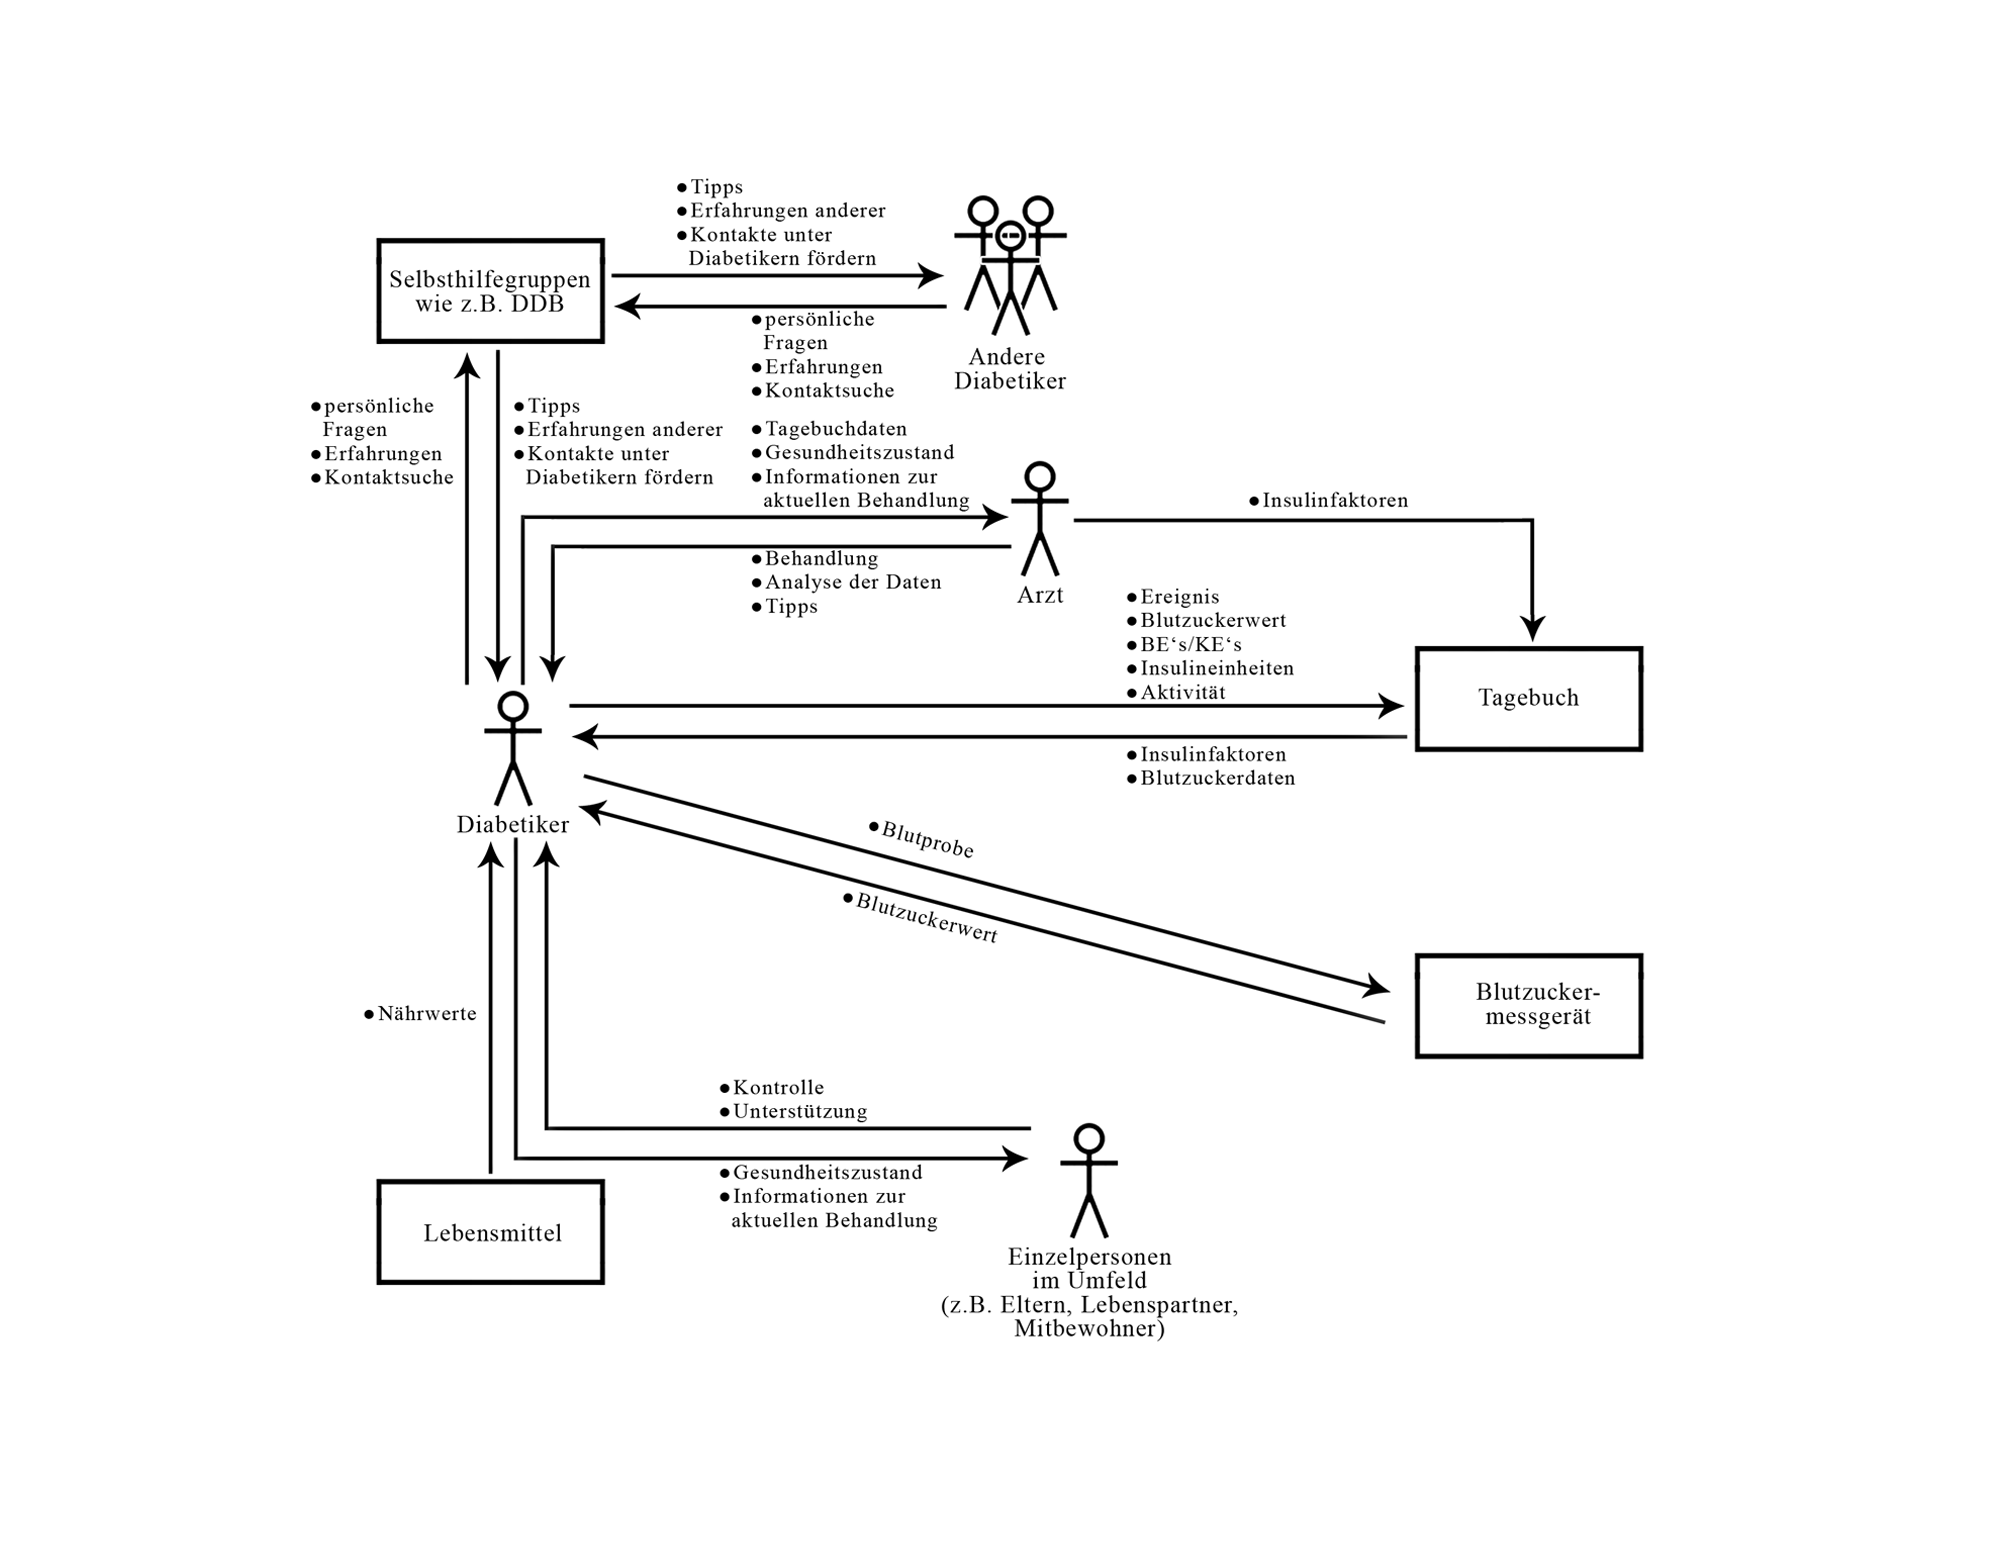
\includegraphics[width=1.0\textwidth]{images/deskriKommDiagramm.png}}
	\captionsetup{justification=centering}
	\caption{Deskriptives Kommunikationsmodell}
	\label{img:deskriptiv}
\end{figure}
\begin{figure}[H]
	\centering
	\setlength{\fboxsep}{1pt}
	\setlength{\fboxrule}{1pt}
	\fbox{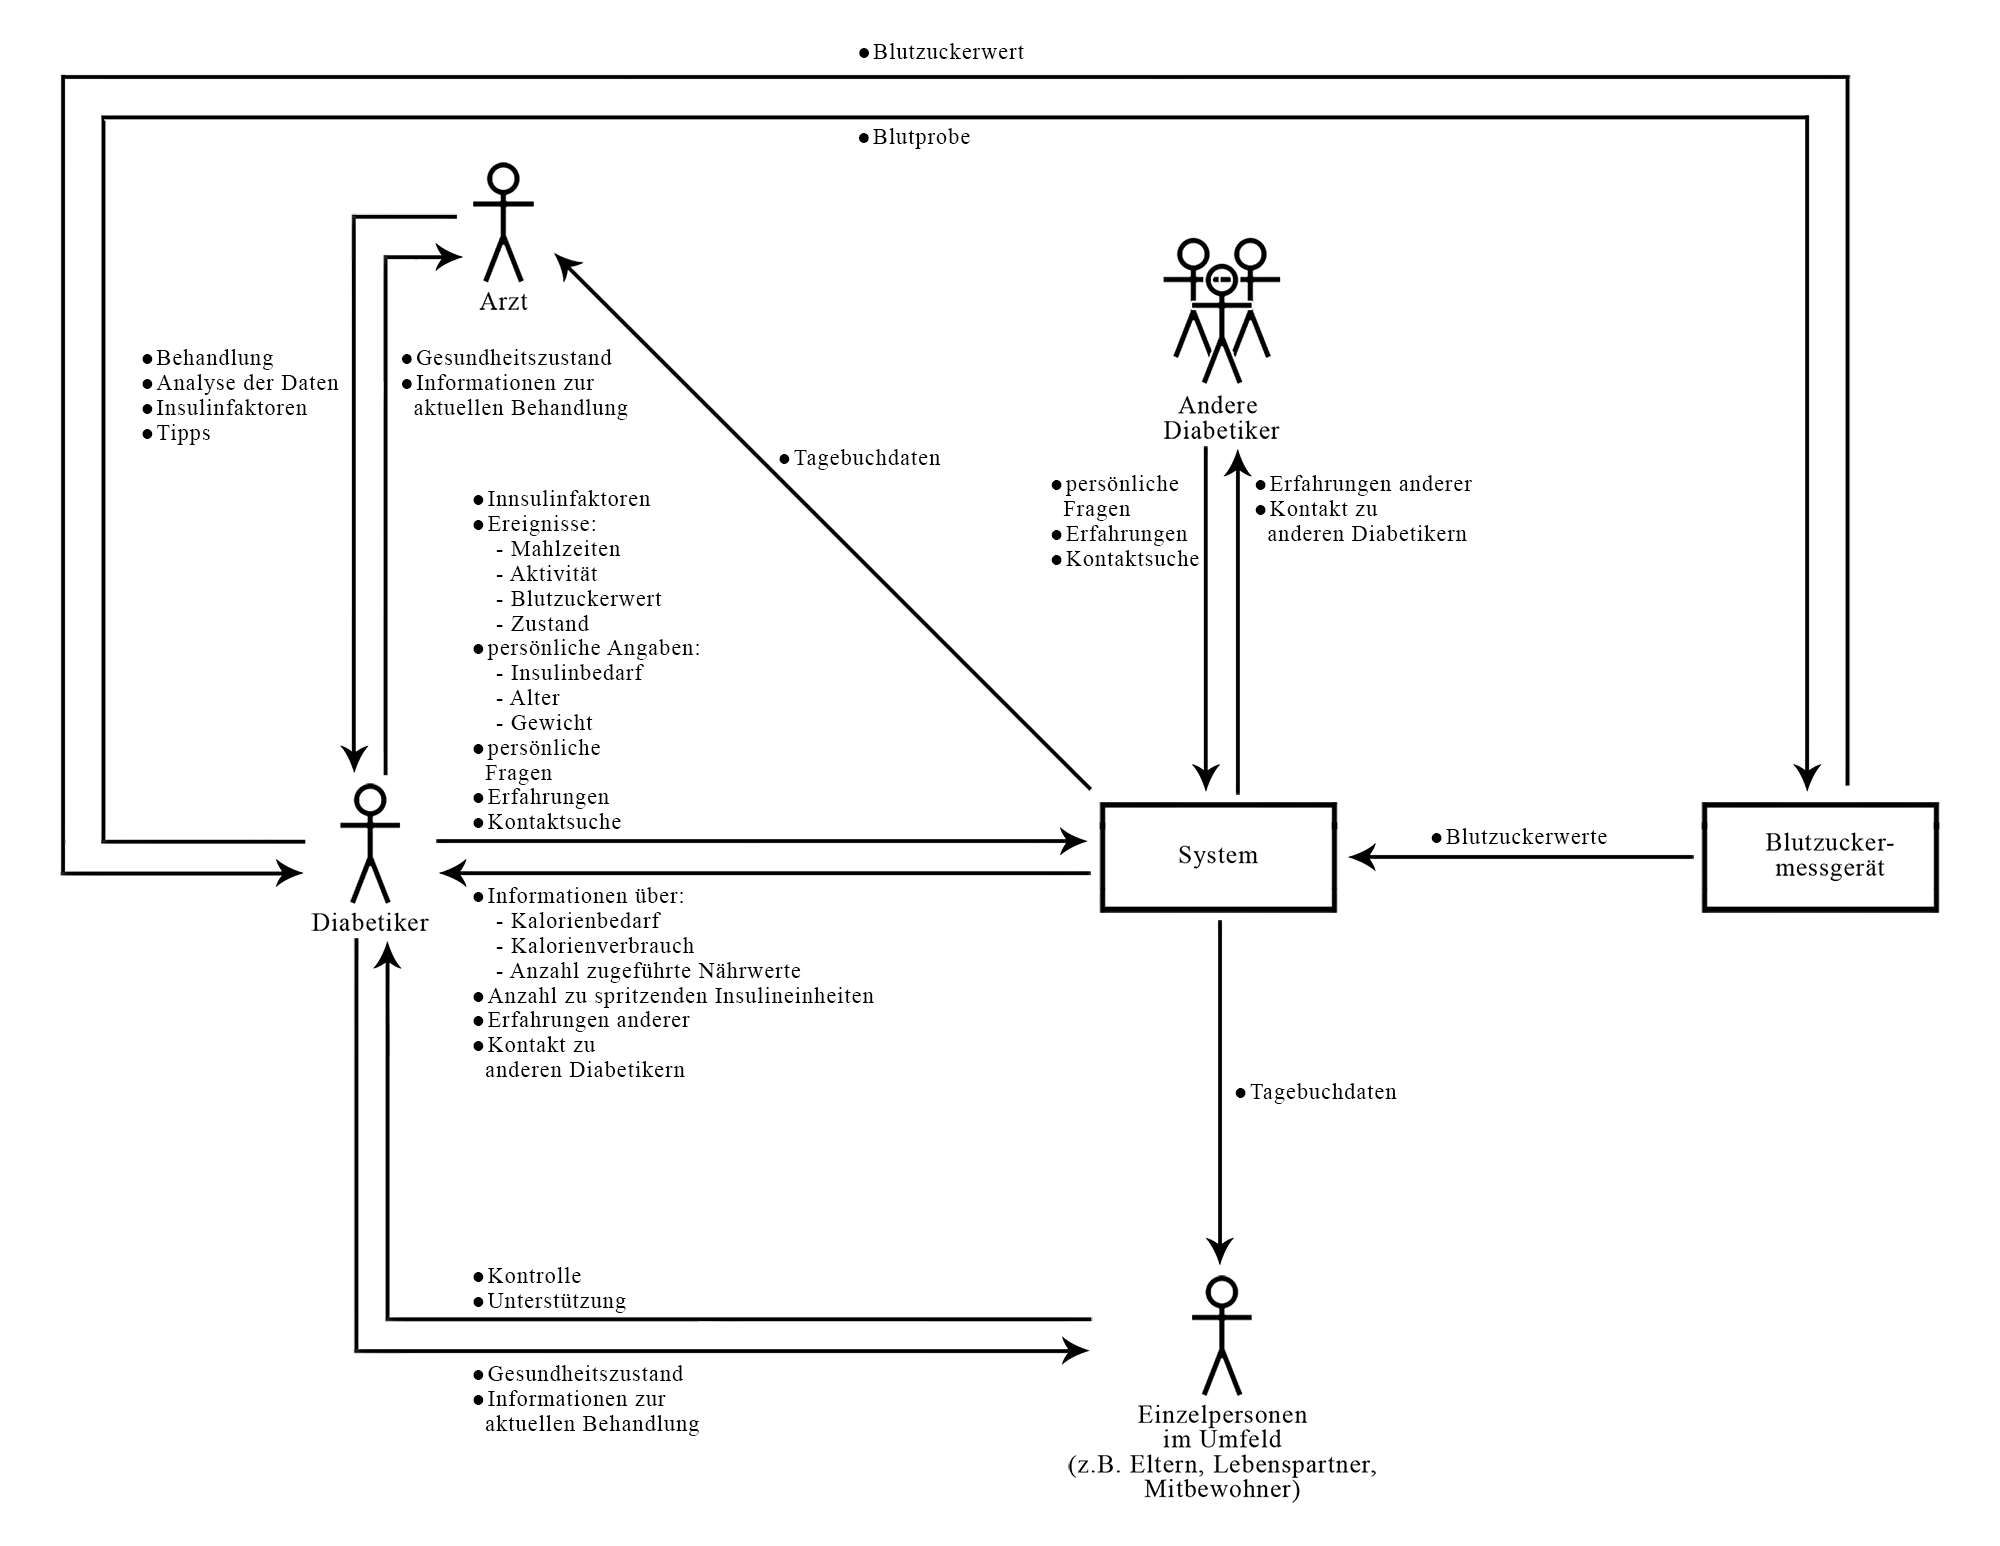
\includegraphics[width=1.0\textwidth]{images/praskriKommDiagramm.png}}
	\captionsetup{justification=centering}
	\caption{Präskriptives Kommunikationsmodell}
	\label{img:präskriptiv}
\end{figure}
	\newpage
	
	\section{Benutzermodellierung}
	Der Usability Engineering Lifecycle nach Mayhew hilft, die Benutzerfreundlichkeit eines Systems (Usability) und das entsprechende Design der Benutzeroberflächen (User Interfaces) zu erreichen. Nach Mayhew wird diese Benutzerfreundlichkeit daran gemessen, wie einfach eine Benutzeroberfläche verwendet und erlernt werden kann. Die Benutzermodellierung ist Teil der „Requirements Analysis“, eine von drei fundamentalen Prozess-Phasen im Usability Engineering Lifecycle und dient zur Anforderungsanalyse. \cite{MD}
	\subsection{Stakeholder-Analysis}
	Um für das zu entwickelnde System eine strukturierte Analyse von Usability-Anforderungen durchführen zu können, muss zunächst die Zielgruppe der Anwerdung bestimmt werden. Zwar lässt sich diese bereits in den früheren Entwicklungsphasen und auch während der erneuten Themenfeldanalyse gut definieren, allerding sind diese Benutzergruppen und ihr Bezug zur Domäne und zum System und  seinen Merkmalen in dieser Phase noch zu überarbeiten und anhand  der Erwartungen und Erfordernisse spezifischer zu definieren.  Mit Hilfe der Stakeholder-Analyse (Tabelle  \ref{tab:Stakeholder}: \nameref{tab:Stakeholder}) werden die Benutzer anhand ihrer Erwartungen und Anforderungen in Kategorien eingeteilt und diese konsequent auf Konflikte hin analysiert.
	\begin{center}
		\begin{longtable}[H]{|p{3cm}|p{2cm}|p{4cm}|p{4.5cm}|}
			\hline
			\textbf{Bezeichnung} & \textbf{Bezug} & \textbf{Objektbereich} & \textbf{Erfordernis/Erwartung}\\
			\hline
			Diabetiker & Anrecht & System & ein Hilfsmittel für den Umgang mit Diabetes\\
			\cline{2-4}
			& Anteil & Merkmal: Datensicherung & von Benutzer eingegebene Daten werden sicher verwaltet\\
			\cline{3-4}
			& & Merkmal: Funktionen zum Tausch von Erfahrungen & um einen Erfahrungsaustausch zwischen Diabetikern zu ermöglichen, sind Erfahrungen von verscheidenen Benutzern essentiell\\
			\cline{2-4}
			& Anspruch & Merkmal: Funktionen zur Dokumentation von Diabetes, Ernährung und Aktivität & ausführliche Dokumenation muss gewährleistet sein\\
			\cline{3-4}
			& & Merkmal: Funktion zur Kontaktaufnahme zu anderen Diabetikern & sozialer Kontakt zu anderen Diabetikern muss gewährleistet sein\\
			\cline{3-4}
			& & Merkmal: Berechnung von Daten & Berechnungen von individuellen Daten müssen gewährleistet sein und korrekt durchgeführt werden\\
			\cline{3-4}
			\newpage
			\cline{3-4}
			& & Merkmal: user interface & Benutzung selbsterklärend, einfach zu lernen, zu merken\\
			\cline{2-4}
			& Interesse & System & Steigerung des Wohlbefindens und der Lebensqualität\\
			\hline
			Personen aus gemeinsamen Haushalt/Umfeld & Anrecht & System & ein Hilfsmittel für die Unterstützung bei Behandlung\\
			\cline{2-4}
			& Anteil & - & - \\
			\cline{2-4}
			& Anspruch & Merkmal: Funktionen zur Berechnung von Nährwerten eines Lebensmittels & Personen (Eltern, Lebenspartner, etc.), die für einen Diabetiker kochen, sollten keine Nährwerte zählen und berechnen müssen\\
			\cline{3-4}
			& & Merkmal: Zugriff auf Blutzuckerdaten eines ausgewählten Diabetikers & die persönlichen Blutzuckerwerte eines Diabetikers sollten einzusehen sein\\
			\cline{3-4}
			& & Merkmal: user interface & Benutzung selbsterklärend, einfach zu lernen, zu merken\\
			\cline{2-4}
			& Interesse & System & Steigerung des Wohlbefindens und der Lebensqualität\\
			\hline 
			Arzt & Anrecht & System & vereinfachte Darstellung der Blutzuckerwerte zur Analyse\\
			\cline{2-4}
			& Anteil & Merkmal: Datensicherung & vom Arzt festgelegte Faktoren können individuell eingespeichert werden\\
			\cline{2-4}
			& Anspruch &  Merkmal: Zugriff auf Blutzuckerdaten eines ausgewählten Diabetikers & die persönlichen Blutzuckerwerte eines Diabetikers sollten einzusehen sein\\
			\cline{3-4}
			& & Merkmal: user interface & Benutzung selbsterklärend, einfach zu lernen, zu merken\\
			\cline{2-4}
			& Interesse & System & Steigung des Wohlbefindens und der Lebensqualität der Patienten\\
			\hline
			\newpage
			\hline
			Krankenkassen & Anrecht & - & -\\
			\cline{2-4}
			& Anteil & System & Übernahme eventueller Kosten für die Nutzung des Systems\\
			\cline{2-4}
			& Anspruch & System & ein finanzierbares System\\
			\cline{2-4}
			& Interesse & System & Patienten bevorzugen Krankenkassen mit einer großteiligen Übernahme der Kosten des Systems\\
			\hline
			Pharmaindustie & Anrecht & - & -\\
			\cline{2-4}
			& Anteil & - & -\\
			\cline{2-4}
			& Anspruch & Medikamenten & Profit durch Verkauf von Medikamenten\\
			\cline{2-4}
			& Interesse & Insulinbedarf & mehr Insulinbedarf der Patienten bedeutet mehr Profit\\
			\hline
			Konkurrenz & Anrecht & - & -\\
			\cline{2-4}
			& Anteil & - & -\\
			\cline{2-4}
			& Anspruch & - & -\\
			\cline{2-4}
			& Interesse & Verkauf von eigenem Produkt & hohe Verkaufszahlen des eigenen Produkts und niedrige Verkaufszahlen der Konkurrenzprodukte\\
			\hline
			Stores für mobile Anwendungen & Anrecht & - & -\\
			\cline{2-4}
			& Anteil & - & -\\
			\cline{2-4}
			& Anspruch & - & -\\
			\cline{2-4}
			& Interesse & Verkauf von Produkt & Profit durch Erwerb des Systems\\
			\hline
			\captionsetup{justification=centering}
			\caption{Stakeholder-Analysis}
			\label{tab:Stakeholder}
		\end{longtable}
	\end{center}
	\setlength{\parindent}{0pt}Mit Hilfe der Tabelle \ref{tab:Stakeholder}: \nameref{tab:Stakeholder} können Diabetiker und Personen aus ihrem Umfeld wie Eltern oder Lebenspartner eindeutig als Zielgruppe des zu entwickelnden Systems identifiziert werden. Die Tabelle zeigt jedoch nicht, dass es zwei verschiedene Arten von Diabetikern gibt (Typ-1- und Typ-2-Diabetiker). Obwohl die beiden Benutzerkategorien dieselben Anforderungen haben, muss eine Unterscheidung nach der Wichtigkeit der Anforderungen getroffen und an das System gestellt werden: Bei Typ-1-Diabetes ist aufgrund der Notwendigkeit einer Insulintherapie die Dokumentation von diabetesrelevanten Daten wie Blutzuckerspiegel, Insulin und Broteinheiten unerlässlich, während bei den Typ-2-Diabetikern Insulinmangel nicht immer die Ursache für eine Erkrankung ist. Vielmehr sind hier eine gesunde Ernährung und regelmäßige Bewegung entscheidend für die Regression dieser Art von Diabetes und die Aufzeichnung und Dokumentation von Mahlzeiten und sportlichen Aktivitäten hat daher einen höheren Stellenwert als die Dokumentation von Insulineinheiten. Aus diesem Grund müssen die verschiedenen Benutzerkategorien bei der Weiterentwicklung berücksichtigt werden.\\
	Neben den Stakeholdern mit ihren positiven Erwartungen an das System oder seine Funktionen gibt es weitere Stakeholder, die möglicherweise in Konflikt mit dem System stehen. Die Pharmaindustrie und Apotheken erzielen Umsatz durch den Verkauf von Medikamenten. Da das zu entwickelnde System den Blutzuckerspiegel konstant regulieren und die Rückbildung des Typ-2-Diabetes bewirken sollte,  hätte die Pharmaindustrie kein großes Interesse an der Entwicklung eines solchen Systems.  Eine Möglichkeit, diesen Interessenkonflikt zu lösen, könnte darin bestehen, Apotheken als Verkaufs- oder Marketingfläche zu nutzen. Die Apotheken könnten durch Werbung und Zusammenarbeit Gewinne ebenfalls erzielen, und die Pharmaindustrie könnte als Kooperationspartner für das Entwicklungsteam fungieren. Wettbewerberunternehmen haben logischerweise auch kein Interesse an der Entwicklung des Systems, da sie den Verkauf ihrer eigenen Produkte den Produkten anderer Unternehmen vorziehen. Auch hier wäre eine Kooperation eine Option zur Konfliktlösung und zur Erweckung von Interessen. Technologien wie Sensoren oder Geräte von Wettbewerbern zu Erfassung von Blutzuckerwerten könnten  über Programmierschnittstellen in Systeme von Drittanbietern mit Gewinnbeteiligung integriert werden. Dies erleichtert die Erfassung von Blutzuckerdaten und macht die Herstellung zusätzlicher Messgeräte überflüssig. Der Wettbewerb generiert auch zusätzliche Gewinne durch die Entwicklung des Systems und die Bereitstellung eigener Schnittstellen.	
	\subsection{User-Profiles}
	Um im weiteren Entwicklungsverlauf die Anforderungen der verschiedenen Benutzerkategorien an das System zu erhalten, werden im Folgenden User Profiles für die definierten Kategorien Typ-1-Diabetiker (Tabelle \ref{tab:User-Profile-1}) und Typ-2-Diabetiker (Tabelle \ref{tab:User-Profile-2}) erstellt. Beim Anlegen dieser User Profiles können Benutzereigenschaften und -merkmale auch aus der bereits durchgeführten Befragung von Probanden aus den beiden Benutzerkategorien (s. Anhang: A \nameref{section:Evaluation} ab Seite \pageref{section:Evaluation}) definiert werden. Diese Merkmale sind wie folgt zu ordnen:
	\begin{itemize}
		\item Physische Merkmale
		\item Psychologische Merkmale
		\item Wissen und Erfahrungen
		\item Aufgabenmerkmale
	\end{itemize}
	Alternativ können Diabetiker Gruppen auch in „Kinder und Jugendliche mit Diabetes“ und „Erwachsene mit Diabetes“ eingeteilt werden. Ergebnisse der bisherigen Recherche zeigen jedoch, dass eine Aufschlüsselung nach Diabetes-Typen eine höhere Priorität hat als die nach Altersgruppen. 
	\subsubsection{Typ-1-Diabetiker}
	\begin{center}
		\begin{longtable}[H]{p{6.6cm}p{6.6cm}}
			\multicolumn{2}{c}{User Profile - Typ-1-Diabetiker} \\
			\toprule
			\multicolumn{2}{l}{User Category Identifiers}\\
			\multicolumn{2}{p{13.6cm}}{Menschen zwischen 5 und 82 Jahren mit Typ-1-Diabetes aus Deutschland kommen nicht aus einer definierten Arbeitsgruppe und haben Keine Erfahrung mit dem Einsatz mobiler Anwendungen.} \\\\
			\textbf{Merkmal} & \textbf{Merkmalsausprägung}\\
			\midrule
			1. Physische Merkmale & \\[.5\normalbaselineskip]
			Geschlecht & \tabitem männlich\\
			& \tabitem weiblich \\ 
			& \tabitem diverse \\[.3\normalbaselineskip]
			Alter & 5-82 Jahre \\[.3\normalbaselineskip]
			Händigkeit & Links- und Rechtshänder \\[.3\normalbaselineskip]
			Wohnort & national (Deutschland)\\[.3\normalbaselineskip]
			Gesundheitszustand & \tabitem Diabetes mellitus Typ 1\\
			& \tabitem Folgeerkrankungen\\
			& \tabitem körperliche Behinderung\\[.3\normalbaselineskip]
			Sozio-ökonomischer Status &  \tabitem Schüler/-in\\
			& \tabitem Studierende-/r \\ 
			& \tabitem Auszubildende-/r\\
			& \tabitem Angestellte-/r\\
			& \tabitem Ausgelehrte./r\\
			& \tabitem Arbeitslose-/r\\
			& \tabitem Berufliche Selbstständigkeit\\[.3\normalbaselineskip]
			Einkommen & \tabitem kein Einkommen\\
			& \tabitem Taschengeld\\
			& \tabitem geregeltes/staatliches Einkommen\\[.3\normalbaselineskip]
			\midrule
			2. Psychologische Merkmale & \\[.5\normalbaselineskip]
			Behandlungsart & \tabitem Insulinspritzen\\
			& \tabitem Insulinpumpe\\[.3\normalbaselineskip]
			Behandlungsziele & \tabitem regulierte Blutzuckerwerte\\
			& \tabitem Vermeidung der Folgeerkrankungen\\
			& 	\tabitem hoche Lebensqualität\\[.3\normalbaselineskip]
			Lebensziele & \tabitem Schul-/Studium-/Ausbildungsabsch-lüsse\\
			& \tabitem Steigung des Wohlbefindens und der Lebensqualität\\
			& \tabitem Weiterbildung\\
			& \tabitem Existenzsicherheit\\
			& \tabitem möglichst lange Lebenszeit\\
			& \tabitem beruflicher Aufstieg\\
			& \tabitem hohe Lebensqualität\\[0.3\normalbaselineskip]
			Motivation zu Nutzung des zukünftigen Systems & \tabitem einfache Handhabung der Diabetes\\
			& \tabitem besser Blutzuckerwerte\\
			& \tabitem keine analoge/schnelle Dokumentation\\
			& \tabitem Abnahme der BE-Berechnung\\
			& \tabitem Abnahme der Insulinberechnung\\
			& \tabitem zeitsparende Anwendungen\\
			& \tabitem Darstellung der Blutzuckerwerte in verständlicher Formen (Graphen oder Tabelle)\\
			& \tabitem Risiko der Folgeerkrankungen reduzieren\\
			& \tabitem Stressreduzierung\\[0.3\normalbaselineskip]
			\midrule
			3. Wissen und Erfahrungen  & \\[.5\normalbaselineskip]
			Erfahrung im Anwendungsgebiet & ausreichend bis sehr gut, durch Schulungen und Eigenbehandlung des Diabetes seit Erkrankung\\[.3\normalbaselineskip]
			Technische Unterstützung bei Therapie & \tabitem Blutzuckermessgerät\\
			& \tabitem Insulinpumpe \\[0.3\normalbaselineskip]
			\midrule
			4. Aufgabenmerkmale & \\[.5\normalbaselineskip]
			Kenntnisse und Fähigkeiten & \tabitem Lesen/Schreiben/Rechnen\\
			& \tabitem Berechnung von Kohlenhydrat, BE's und Insulineinheiten\\
			& \tabitem Diabetes-Dokumentation\\ 
			& \tabitem Nutzung von verfügbaren Technologien\\[0.3\normalbaselineskip]
			Verfügbare relevante Technologien & \tabitem Smartphones\\
			& \tabitem Smartwatches\\
			& \tabitem Tablets\\[0.3\normalbaselineskip]
			
			\bottomrule
			\captionsetup{justification=centering}
			\caption{User Profile: Typ-1-Diabetiker}
			\label{tab:User-Profile-1}
		\end{longtable}
	\end{center}
	\subsubsection{Typ-2-Diabetiker}
	\begin{center}
		\begin{longtable}[H]{p{6.6cm}p{6.6cm}}
			\multicolumn{2}{c}{User Profile - Typ-2-Diabetiker} \\
			\toprule
			\multicolumn{2}{l}{User Category Identifiers}\\
			\multicolumn{2}{p{13.6cm}}{Menschen aus Deutschland, von denen die meisten im Erwachsenenalter an Typ-2-Diabetes erkrankt sind, in den letzten Jahren auch zunehmend im Jugendalter, kommen aus keiner definierten Arbeitsgruppe und haben Erfahrung mit dem Einsatz mobiler Anwendungen.} \\\\
			\textbf{Merkmal} & \textbf{Merkmalsausprägung}\\
			\midrule
			1. Physische Merkmale & \\[.5\normalbaselineskip]
			Geschlecht & \tabitem männlich\\
			& \tabitem weiblich \\ 
			& \tabitem diverse \\[.3\normalbaselineskip]
			Alter & 16-82 Jahre \\[.3\normalbaselineskip]
			Händigkeit & Links- und Rechtshänder \\[.3\normalbaselineskip]
			Wohnort & national (Deutschland)\\[.3\normalbaselineskip]
			Gesundheitszustand & \tabitem Diabetes mellitus Typ 1\\
			& \tabitem Folgeerkrankungen\\
			& \tabitem körperliche Behinderung\\
			& \tabitem Fettleibigkeit\\
			& \tabitem schlechter Ernährungsstil\\[.3\normalbaselineskip]
			Sozio-ökonomischer Status &  \tabitem Schüler/-in\\
			& \tabitem Studierende-/r \\ 
			& \tabitem Auszubildende-/r\\
			& \tabitem Angestellte-/r\\
			& \tabitem Ausgelehrte./r\\
			& \tabitem Arbeitslose-/r\\
			& \tabitem Berufliche Selbstständigkeit\\[.3\normalbaselineskip]
			Einkommen & \tabitem kein Einkommen\\
			& \tabitem Taschengeld\\
			& \tabitem geregeltes/staatliches Einkommen\\[.3\normalbaselineskip]
			\midrule
			2. Psychologische Merkmale & \\[.5\normalbaselineskip]
			Behandlungsart & \tabitem Tabletten\\
			& \tabitem Diät\\
			& \tabitem bei Bedarf Insulintherapie\\[.3\normalbaselineskip]
			Behandlungsziele & \tabitem Körpergewichtreduzierung\\
			& \tabitem ausgewogene Ernährung\\
			& \tabitem regulierte Blutzuckerwerte\\
			& \tabitem Vermeidung der Folgeerkrankungen\\
			& 	\tabitem hoche Lebensqualität\\[.3\normalbaselineskip]
			Lebensziele & \tabitem Schul-/Studium-/Ausbildungsabsch-lüsse\\
			& \tabitem Steigung des Wohlbefindens und der Lebensqualität\\
			& \tabitem Weiterbildung\\
			& \tabitem Existenzsicherheit\\
			& \tabitem möglichst lange Lebenszeit\\
			& \tabitem beruflicher Aufstieg\\
			& \tabitem hohe Lebensqualität\\[0.3\normalbaselineskip]
			Motivation zu Nutzung des zukünftigen Systems & \tabitem einfache Handhabung der Diabetes\\
			& \tabitem Reduzierung des Körpergewichts\\
			& \tabitem Rückbildung der Erkrankung\\
			& \tabitem stabile Blutzuckerwerte\\
			& \tabitem keine analoge/schnelle Dokumentation\\
			& \tabitem zeitsparende Anwendungen\\
			& \tabitem Risiko der Folgeerkrankungen reduzieren\\
			& \tabitem Stressreduzierung\\[0.3\normalbaselineskip]
			\midrule
			3. Wissen und Erfahrungen  & \\[.5\normalbaselineskip]
			Erfahrung im Anwendungsgebiet & keine bis sehr gut, durch ärztliche Unterstützung und Eigenbehandlung des Diabetes seit Erkrankung\\[.3\normalbaselineskip]
			Technische Unterstützung bei Therapie & \tabitem Blutzuckermessgerät\\[0.3\normalbaselineskip]
			\midrule
			4. Aufgabenmerkmale & \\[.5\normalbaselineskip]
			Kenntnisse und Fähigkeiten & \tabitem Lesen/Schreiben/Rechnen\\
			& \tabitem Diabetes-Dokumentation\\ 
			& \tabitem Nutzung von verfügbaren Technologien\\[0.3\normalbaselineskip]
			Verfügbare relevante Technologien & \tabitem Smartphones\\
			& \tabitem Smartwatches\\
			& \tabitem Tablets\\[0.3\normalbaselineskip]
			\bottomrule
			\captionsetup{justification=centering}
			\caption{User Profile: Typ-2-Diabetiker}
			\label{tab:User-Profile-2}
		\end{longtable}
	\end{center}
	Es empfiehlt sich, in der Benutzermodellierung auf der Grundlage des Benutzerprofils sogenannte Personas zu entwerfen, um reale Personen in einer fiktiven Darstellung in die Modellierung einzubeziehen. Zwar ist dies im Usability Engineering Lifecycle nicht vorgegeben und optional, allerdings bieten Personas eine Grundlage für die spätere Aufgabenmodellierung. Es wird folglich jeweils ein Persona zum User Profil der Typ-1 und der Typ-2-Diabetiker angefertigt. Die erste Persona wird in Anlehnung der Dokumentation von Journal Stuttgart - RegioTV „Leben mit Diabetes“ vom 15.08.2018 und die zweite in Anlehung der Dokumentation von NDR Ratgeber „Typ-2-Diabetes: Wie man vom Insulin wieder wegkommt | Die Ernährungs-Docs | NDR“ verfasst. 
	\subsection{Personas}
	\textbf{Persona - Typ-1-Diabetiker}
	\begin{center}
		\begin{longtable}[H]{p{6.6cm}p{6.6cm}}
			\addtocounter{table}{-1}
			\texttt{Name: }& \texttt{Lucie}\\
			\texttt{Alter: }& \texttt{6 Jahre}\\
			\texttt{Geschlecht: }&\texttt{weiblich}\\
			\texttt{Wohnort:} & \texttt{Stuttgart, bei ihren Eltern}\\
			\texttt{Gesundheitszustand:} & \texttt{Diabete-mellitus-Typ-1}\\
			\texttt{Sozio-ökonomischer Status: }& \texttt{Schülerin}\\
			\texttt{Behandlungsart:} & \texttt{Insulinpumpe}\\
			&  \texttt{stündliche Blutzuckermessung}\\
			&  \texttt{analoges Tagebuch}\\
			\texttt{Behandlungsziel:} &  \texttt{Diabetes kontrollieren}\\
			&  \texttt{ein normales Leben}\\
			\texttt{Erfahrungen: }&  \texttt{seit 3 Jahren an Diabetes erkrankt}\\
			&  \texttt{Erfahrung der Eltern und Betreuer durch Schulungen in Krankenhäuser}\\
			\texttt{Technische Unterstützung:} & \texttt{FreeStyle-Libre Blutzuckermessgerät}\\
			&  \texttt{Insulinpumpe}\\
		\end{longtable}
	\end{center}
	\texttt{Lucie ist 6 Jahre alt und seit 3 Jahren an Diabetes mellitus Typ 1 \newline
		erkrankt. Gleich am Morgen wird Lucie mit ihrer Krankheit konfrontiert, \newline 
		denn ein Leben wie ein gesundes Kind wird sie nicht mehr leben können. \newline
		Noch vor dem Frühstück misst sie gemeinsam mit ihrer Mutter ihren \newline
		Blutzuckerspiegel. Fast alle  Aufgaben in ihrer Diabetesbehandlung macht \newline 
		sie gemeinsam mit ihren Eltern. Ihre Mutter musste nach der Erkrankung \newline
		von Lucie ihre Arbeit kündigen, um jederzeit abrufbereit zu sein.}\newline
		 \texttt{Lucie schnappt sich ihr Blutzuckermessgerät und legt es auf ihren\newline
		 	 FreeStyle Libre-Sensor am Oberarm. Ihr Blutzuckerspiegel ist in einem \newline 
		 	 gesunden Bereich. Als es an den Frühstückstisch geht, muss Lucies Mutter \newline
		 	 sie an das Spritzen des Insulins für die Mahlzeit erinnern. Gemeinsam \newline
		 	 schnappen sie sich die  Wage, wiegen die Scheibe Vollkornbrot \newline
		 	 und den Apfel und ermitteln anhand der Kohlenhydrate die Broteinheiten\newline
		 	  und Insulineinheit, die Lucie spritzen muss. Sie zückt ihre \newline
		 	 Insulinpumpe und trägt die Insulineinheiten ein, die ihre Mutter \newline
		 	 ihr vorgerechnet hat. Aber auch nach dem Spritzen des Insulins muss \newline 
		 	 sich Lucie noch einige Minuten gedulden. Denn wenn sie direkt essen \newline
		 	 würde, würde sie den nötigen Spritz-Ess-Abstand von 10 Minuten nicht \newline
		 	 einhalten und  die Kohlenhydrate des Essens würden schneller wirken \newline
		 	 als das Insulin. }\newline
		\texttt{Nachdem Lucie ihr Frühstück verspeist und ihre Schulsachen \newline
			zusammengepackt hat, fährt Lucies Mutter sie in die Schule. \newline
			Lucie besucht eine ganz besondere Schule. Sie besucht die Waldschule \newline
			in Stuttgart. Die Waldschule ist die erste Schule, die Schulklassen aus \newline
			Schülern mit Diabetes gebildet hat. Neben diesen Klassen gehen auch \newline
			gesunde Schüler zur Waldschule. Lucies Eltern sind froh, dass es diese \newline
			 Schule gibt, auch wenn sie monatlich 160\euro für diese zahlen  müssen. \newline
			 Bereits bei der Suche eines Kitaplatzes hatten Lucies Eltern große \newline
			 Probleme und erhielten auf Nachfrage einige Absagen. An der Waldschule \newline
			 werden die Schüler von geschulten Lehrer unterrichtet und von \newline
			 Diabetesassistenten und Krankenschwestern betreut, die Fachwissen\newline
			  besitzen und immer mit nötiger Sicherheit in Situation handeln können. \newline
			  Dennoch ist Lucie auch während der Schulzeit und ihrer Freizeit \newline
			  dazu verpflichtet, den Diabetes zu kontrollieren. Zur Sicherheit trägt sie \newline
			  immer eine kleine Tasche mit Süßigkeiten, Blutzuckermessgerät\newline
			   und Notfallspritzen bei sich mit. Blutzuckermessungen  führt sie \newline
			   stündlich durch. Während den großen Pausen und dem Sportunterricht besteht \newline
			   wegen der Bewegung die Gefahr eines niedrigen Blutzuckerspiegels. Hierzu \newline
			   misst Lucie sogar alle 20-30 Minuten ihren Blutzucker und isyt vor dem Sport \newline
			   eine Banane oder Traubenzucker. Wenn sie während der Schulzeit ihren \newline
			   Blutzuckerspiegel misst, trägt sie diesen und auch ihre Mahlzeiten in ihr \newline
			   analoges Tagebuch ein, damit ihre Eltern nach der Schule diese kontrollieren können.\newline
			    Lucie kann ihre Erkrankung und ihre Blutzuckerwerte schon sehr gut \newline
			    einschätzen, allerding wünscht sie sich sehr oft, einfach ein normales \newline
			    Leben leben zu können. }\\
		    
		    
		    \textbf{Persona - Typ-2-Diabetiker}
		    \begin{center}
		    	\begin{longtable}[H]{p{6.6cm}p{6.6cm}}
		    		\addtocounter{table}{-1}
		    		\texttt{Name: }& \texttt{Bernd Pache}\\
		    		\texttt{Alter: }& \texttt{53 Jahre}\\
		    		\texttt{Geschlecht: }&\texttt{männlich}\\
		    		\texttt{Wohnort:} & \texttt{Hamburg}\\
		    		\texttt{Gesundheitszustand:} & \texttt{Diabete-mellitus-Typ-2}\\
		    		\texttt{Sozio-ökonomischer Status: }& \texttt{Schulleiter}\\
		    		\texttt{Behandlungsart:} & \texttt{Insulinspritze}\\
		    		&  \texttt{Tabletten}\\
		    		\texttt{Behandlungsziel:} &  \texttt{Insolinlose Behandlung}\\
		    		&  \texttt{Körpergewicht reduzieren}\\
		    		\texttt{Erfahrungen: }&  \texttt{seit 8 Jahren an Diabetes erkrankt}\\
		    		&  \texttt{Schulungen zur Ernährung}\\
		    	\end{longtable}
		    \end{center}
		    \texttt{Bernd Pache ist 53 Jahre alt und leidet seit 8 Jahren an Diabetes mellitus \newline
		    	Typ 2. Da seine Muskelzellen inzwischen eine sehr geringe Insulin-\newline
		    	empfindlichkeit aufweisen und das vom Körper produzierte \newline
		    	Insulin nicht ausreicht, muss der Schulleiter aus Hamburg neben der \newline
		    	Einnahme von Tabletten auch täglich Insulin spritzen. Dieses Insulin \newline
		    	reduziert zwar den Blutzuckerspiegel, sorgt allerdings auch für ein \newline
		    	höheres Risiko dauerhaft das Körpergewicht zuzunehmen. Senkt das \newline
		    	Insulin den Blutzuckerspiegel zu sehr und Bernd unterzuckert, \newline
		    	bekommt er Hunger und muss etwas essen. Isst Bernd dann mehr\newline
		    	als für die Unterzuckerung notwendig war, muss er erneut Insulin spritzen.\newline
		    	Ein Teufelskreis. Nach 4 Jahren Insulinbehandlung und 20 kg \newline
		    	Gewichtszunahme möchte Bernd sein Lebensstil ändern und so \newline
		    	schnell wie möglich das Spritzen von Insulin absetzten. Um dies umsetzten\newline
		    	zu können, gilt es sich ausgewogen zu Ernähren und regelmäßig Sport zu \newline
		    	treiben. Gefährliche Kombinationen aus Kohlenhydrate und Fett darf Bernd \newline
		    	nicht mehr zu sich nehmen. Stattdessen stehen viel Eiweiß, viel Gemüse \newline
		    	und keine Süßigkeiten auf den Speiseplan. Seine Kohlenhydrate-, \newline
		    	Eiweiß- und Fettaufnahme muss Bernd ebenfalls im Auge behalten. \newline
		    	Nach 6 Monaten bewusster Ernährung, aus überwiegend Obst und Gemüse,\newline
		    	und regelmäßigem Sport sind bereits erstaunliche Erfolge zu sehen. \newline
		    	Bernd hat insgesamt 21 kg Körpergewicht	verloren und konnte das \newline
		    	Insulinspritzen bereits nach 2 Monaten einstellen. Auch seine \newline
		    	Blutzuckerwerte haben sich verbessert. Sein HbA1c-Wert ist \newline
		    	von 8\% auf 6,8\% gesunken. Führt Bernd auch weiterhin den Lebensstil \newline
		    	wie in den vergangenen 6 Monaten, ist das Halbieren oder sogar \newline
		    	Absetzen der Tablettendosis das neue Ziel.}
	
	\subsection{Anforderungen}
	Um anhand der User Profiles und der Personas eine kontextbezogene Aufgabenanalyse (Contextual Task Analysis) erstellen und die Nutzung des Systems modellieren zu können, müssen zunächst einige Funktionen des zukünftigen Systems identifiziert werden. Dazu müssen mit Hilfe der Stakeholder-Analysis und der User Profiles Systemanforderungen erstellt werden.
	Die Anforderungen werden durch Modellierung der Benutzer in Form von Stakeholder-Analysen, Benutzerprofilen und Personas beschrieben. Sie lassen sich in funktionale und non-funktionale Anforderungen unterteilen. Die funktionalen Anforderungen müssen den wesentlichen Benutzerkategorien zugeordnet werden, für die User Profiles zuvor erstellt wurden.
	\subsubsection{funktionale Anforderungen}
	\paragraph{Für alle Diabetiker}\mbox{}
	\begin{itemize}
		\item\textbf{\lbrack F10\rbrack} Das System muss dem Benutzer die Möglichkeit bieten, ein individuelles Benutzerkonto anzulegen.
		\item\textbf{\lbrack F20\rbrack}  Das System muss dem Benutzer die Möglichkeit bieten, die individuellen Daten seines Benutzerkontos zu bearbeiten.
		\item\textbf{\lbrack F30\rbrack} Das System muss dem Benutzer die Möglichkeit bieten, sein angelegtes Benutzerkonto wieder zu löschen.
		\item\textbf{\lbrack F40\rbrack}	Das System kann dem Benutzer die Möglichkeit bieten, Blutzuckerwerte die von externen Blutzuckermessgeräten erfasst wurden per API in das System zu übernehmen.
		\item\textbf{\lbrack F50\rbrack}	Das System muss dem Benutzer die Möglichkeit bieten, unterschiedliche Ereignisse (Blutzuckerwert, Mahlzeit und sportliche Aktivität) manuell in das Tagebuch einzutragen.
		\item\textbf{\lbrack F50\rbrack} Das System soll dem Benutzer die Ereignisse und Blutzuckerwerte in Form von Tagebucheinträgen und anhand eines Graphen repräsentieren.
		\item\textbf{\lbrack F70\rbrack} Falls ein Ereignis bereits vorhanden ist, soll das System dem Benutzer die Möglichkeit bieten, diesen zu ändern oder um weitere Daten zu erweitern zu können.
		\item\textbf{\lbrack F80\rbrack} Das System soll dem Benutzer die Möglichkeit bieten, auf eine Lebensmittel-Datenbank zugreifen zu können.
		\item\textbf{\lbrack F90\rbrack} Das System soll dem Benutzer die Möglichkeit bieten, erfasste Aktivitäten durch andere Anwendungen einzupflegen.
		\item\textbf{\lbrack F100\rbrack} Das System muss dem Benutzer die Möglichkeit bieten, Aktivitäten hinzuzufügen.
		\item\textbf{\lbrack F110\rbrack} Das System soll dem Benutzer den Kalorienbedarf, bestehend aus Grundumsatz und Leistungsumsatz, repräsentieren.
		\item\textbf{\lbrack F120\rbrack} Das System muss dem Benutzer die Möglichkeit bieten, Kontakt zu anderen Benutzern in einer Kommunikationsplattform herzustellen.
		\item\textbf{\lbrack F130\rbrack} Das System muss dem Benutzer die Möglichkeit bieten, Beiträge hinzuzufügen, zu entfernen und zu bearbeiten.
		\item\textbf{\lbrack F140\rbrack} Das System soll dem Benutzer Beiträge andere Benutzer repräsentieren.
		\item\textbf{\lbrack F150\rbrack} Das System soll dem Benutzer die Möglichkeit bieten, Beiträge anderer Benutzer zu kommentieren.
		\item\textbf{\lbrack F160\rbrack} Das System soll dem Benutzer die Möglichkeit bieten, Beiträge andere Benutzer zu bewerten.
		\item\textbf{\lbrack F170\rbrack} Das System soll dem Benutzer die Möglichkeit bieten, durch Aktivität in der Kommunikationsplattform Erolgspunkte zu sammeln.
		\item\textbf{\lbrack F180\rbrack} Das System muss dem Benutzer die Möglichkeit bieten, verschiedene Benutzeroberflächen und Funktionen für verschiedene Benutzergruppen zu benutzen.
		\item\textbf{\lbrack F190\rbrack} Das System soll den Benutzer die Möglichkeit bieten, seine Tagebuch-Einträge in Form einer Tabelle als PDF-Datei zu exportieren und an einer beliebigen E-Mail-Adresse zu senden.
		\item\textbf{\lbrack F200\rbrack} Falls ein zweiter Benutzer um Erlaubnis des Einblicks in die Blutzuckerwerte eines Benutzers gefragt hat, muss das System dem Benutzer die Möglichkeit bieten, die Erlaubnis zu erteilen oder abzulehnen.
	\end{itemize}
	\paragraph{Für Typ-1-Diabetiker}\mbox{}
	\begin{itemize}
		\item\textbf{\lbrack F210\rbrack} Falls der Benutzer eine Mahlzeit als Ereignis hinzufügt, muss das System dem Benutzer die Möglichkeit bieten, die BE's und Insulineinheiten anhand der Kohlenhydrate der Mahlzeit und der Benutzerdaten zu berechnen.
		\item\textbf{\lbrack F220\rbrack} Das System muss dem Benutzer die Möglichkeit bieten, individuellen Insulin- und Korrekturfaktoren anzulegen.
		\item\textbf{\lbrack F230\rbrack} Das System muss dem Benutzer die Möglichkeit bieten, feste Insulinzunahmen anzulegen.
		\item\textbf{\lbrack F240\rbrack} Das System muss dem Benutzer die Möglichkeit bieten, feste Insulinzunahmen zu bearbeiten.
		\item\textbf{\lbrack F250\rbrack} Das System muss dem Benutzer die Möglichkeit bieten, feste Insulinzunahmen zu entfernen.
		\item\textbf{\lbrack F260\rbrack} Das System muss dem Benutzer die Möglichkeit bieten, feste Insulinzunahmen einzusehen.
	\end{itemize}
	\paragraph{Für Typ-2-Diabetiker}\mbox{}
	\begin{itemize}
		\item\textbf{\lbrack F270\rbrack} Das System muss dem Benutzer die Möglichkeit bieten, die Art der Behandlung festzulegen.
		\item\textbf{\lbrack F280\rbrack} Das System soll dem Benutzer die Möglichkeit bieten, sein Zielkörpergewicht anzugeben.
	\end{itemize}
	\paragraph{Für Personen im Umfeld (Eltern, Lebenspartner-/in, ...)}\mbox{}
	\begin{itemize}
		\item\textbf{\lbrack F10\rbrack} Das System muss dem Benutzer die Möglichkeit bieten, ein individuelles Benutzerkonto anzulegen.
		\item\textbf{\lbrack F20\rbrack}  Das System muss dem Benutzer die Möglichkeit bieten, die individuellen Daten seines Benutzerkontos zu bearbeiten.
		\item\textbf{\lbrack F30\rbrack} Das System muss dem Benutzer die Möglichkeit bieten, sein angelegtes Benutzerkonto wieder zu löschen.
		\item\textbf{\lbrack F40\rbrack} Das System muss dem Benutzer die Möglichkeit bieten, unterschiedliche Ereignisse (Blutzuckerwert, Mahlzeit und sportliche Aktivität) manuell in das Tagebuch einzutragen.
		\item\textbf{\lbrack F290\rbrack} Das System muss dem Benutzer die Möglichkeit bieten, verschiedene Benutzeroberflächen und Funktionen für verschiedene Benutzergruppen zu benutzen.
		\item\textbf{\lbrack F300\rbrack} Das System muss dem Benutzer die Möglichkeit bieten, um Erlaubnis des Einblicks in die Blutzuckerwerte eines zweiten Benutzers zu fragen.
		\item\textbf{\lbrack F310\rbrack} Falls der Benutzer die Erlaubnis eines zweiten Benutzers erhalten hat, muss das System dem Benutzer die Möglichkeit bieten, Einblick in Blutzuckerwerte des zweiten Benutzers zu haben.
	\end{itemize}
\subsubsection{Non-funktionale Anforderungen}
\label{section:nfAnforderungen}
\paragraph{Qualitätsanforderungen}
\begin{itemize}
	\item\textbf{\lbrack Q10\rbrack} Das System soll dem Benutzer eine Aufgabenerfüllung innerhalb der Genauigkeits- und Vollständigkeitsgrenzen bieten. (Effektivität)
	\item\textbf{\lbrack Q20\rbrack} Das System soll dem Benutzer eine Aufgabenerfüllung in Bezug auf den Benutzeraufwand bieten. (Effizienz)
	\item\textbf{\lbrack Q30\rbrack} Das System soll dem Benutzer eine von Beeinträchtigungen freie Nutzung und mit einer positiven Einstellung gegenüber dieser bieten. (Zufriedenstellend)
	\item\textbf{\lbrack Q40\rbrack} Das System soll dem Benutzer eine effektive, effiziente und zufriedenstellende Aufgabenerfüllung bieten. (Gebrauchstauglichkeit)
	\item\textbf{\lbrack Q50\rbrack} Das System soll zu 99,9\% erreichbar sein und eine gewisse Ausfallsicherheit garantieren.
	\item\textbf{\lbrack Q60\rbrack} Das System soll über eine strukturierte Benutzeroberfläche mit intuitiver Benutzerführung verfügen.
	\item\textbf{\lbrack Q70\rbrack} Das System muss dem Benutzer fehlerfreie Ergebnisse und Informationen bieten.
\end{itemize}
\paragraph{Organisationale Anforderungen}
\begin{itemize}
	\item\textbf{\lbrack O10\rbrack} Das System soll sensible Daten sicher und unerreichbar für Dritte speichern.
	\item\textbf{\lbrack O20\rbrack} Das System soll einen verlustfreien Datentransport zwischen den verschiedenen Systemkomponenten gewehrleisten.  
	\item\textbf{\lbrack O30\rbrack} Das System soll einen geringen Akkuverbrauch aufweisen.
	\item\textbf{\lbrack O40\rbrack} Das System muss jeder Zeit Kontakt zum Benutzer aufnehmen können.
	\item\textbf{\lbrack O50\rbrack} Das System muss dem Benutzer einen schnellen Zugriff auf den aktuelle Daten bieten.  
\end{itemize}
	Diese Anforderungen werden in den folgenden Aufgaben direkt zum Treffen von Entscheidungen für das User Interface Design verwendet.
	\newpage
	
	\section{Aufgabenmodellierung}

Die Contextual Task Analysis im Usability Engineering Lifecycle dient der Aufgabenanalyse innerhalb der Arbeiten der Benutzer eines Projektes. Nach Mayhew \cite{MD} ist die Analyse der Benutzeraufgaben in den folgenden drei Schritten durchzuführen:
\begin{itemize}
	\item Sammeln von Hintergrundinformationen über die zu automatisierende Arbeit.
	\item Sammeln und Analysieren von Daten aus kontextbezogenen Beobachtungen und Interviews von Benutzern, die in ihrer Arbeitsumgebung arbeiten.
	\item Erstellen des „User Task Organization Model“ anhand der Aufgaben eines Benutzers einer Arbeit.
\end{itemize}

Um Hintergrundinformation über die Arbeit der Benutzer zu erhalten, werden Erkenntnisse aus der Evaluation (s. Anhang: A \nameref{section:Evaluation} ab Seite \pageref{section:Evaluation}) und aus den Dokumentationen (von Journal Stuttgart - RegioTV „Leben mit Diabetes“ und NDR Ratgeber „Typ-2-Diabetes: Wie man vom Insulin wieder wegkommt | Die Ernährungs-Docs | NDR“) die bereits in den Personas verwendet wurden, einbezogen.\newline
In der Aufgabenmodellierung wird zunächst anhand Persona Use Cases und einem Task Scenario die deskreptive Arbeit der Benutzer ohne das zu entwickelnde System analysiert und anschließen durch das Task Organization Model repräsentiert. Um nun eine Aufgabemodellierung hinsichtlich des zu entwickelnden System durchzuführen werden präskriptive Concrete Use Cases, welche die zukünftige Interaktion der Benutzer mit dem System beschreiben, verfasst. 

\subsection{Persona Use Cases (OUC)}

\begin{center}
	\begin{longtable}[H]{|p{2cm}|p{2cm}|p{3cm}|p{3.5cm}|p{2.5cm}|}
		\hline	
		\textbf{Actor} & \textbf{Trigger} & \textbf{Use Case} & \textbf{Task Scenario} & \textbf{Errors,} \\
		\textbf{(User)} &  & \textbf{(Task)} & \textbf{Sequence} & \textbf{Problems, Comments}\\
		\hline	
		Diabetiker & Unwohlge- fühl & OUC 01 Blutzuckerwert messen& 1. Messgerät einschalten und Teststreifen einführen. \newline2. Finger desinfizieren.\newline 3. In den Finger stechen und Blut abtupfen. \newline 4. Blutprobe auf Teststreifen geben. \newline 5. Blutzuckerwert vom Messgerät ablesen.  & Es sollte mindestens 4 mal pro Tag gemessen werden.\newline \newline Alternative Blutgewebemessung mit Sensor.\\
		\cline{2-5}
		& Unter- zuckerung & OUC 02 Unterzuckerung behandeln & 1. Differenz zwischen Blutzuckerwert und Zielwert berechnen. \newline 2. Differenz durch Korreturfaktor teilen, um BE/KE-Anzahl zu erhalten.  \newline  3. BE's/KE's in Form von Einfachzucker essen.& Korrekturfaktor ist indivituell. \newline \newline Bei Unterzuckerung unter 70 mg/dL (4.0 mmol/L) reagieren.\\
		\cline{2-5}
		& Über- zuckerung & OUC 03 Überzuckerung behandeln & 1. Differenz zwischen Blutzuckerwert und Zielwert berechnen. \newline2. Differenz durch Korreturfaktor teilen, um Insulineinheiten zu erhalten. \newline 3. Insulineinheiten spritzen. & Korrektur- faktor  ist indivituell. \newline  \newline Bei Überzuckerung über 180 mg/dL (10.0 mmol/L) reagieren. \\
		\cline{2-5}
		& Hunger & OUC 04 Essen & 1. Mahlzeit wiegen. \newline 2. Kohlenhydrate anhand des Gewichtes der Nahrungsmittel berechnen. \newline  3. Kohlenhydrate in BE/KE umrechnen. \newline 4. BE/KE mit Faktor multiplizieren um Insulineinheiten zu ermitteln. \newline 5. Insulineinheiten spritzen. \newline 6. Spritz-Ess-Abstand einhalten. \newline Essen. & Wenn keine Wage vorhanden, wird geschätzt. \newline \newline Spritz-Ess-Abstand muss eingehalten werden, sonst steigt der Blutzuckerwert bevor das Insulin wirkt.\newline \newline Wenn der Blutzuckerwert vor der Mahlzeit über 250 mg/dL (14.0 mmol/L), darf nicht gegessen werden.\\
		\cline{2-5}
		& Sportliche Bewegung & OUC 05 Sport & 1. Blutzuckermessen. \newline 2. Sport-BE/-KE essen. \newline 3. Alle 20-30 Minuten Blutzucker messen. & Wenn der Blutzuckerwert unter 70 mg/dL (4.0 mmol/L) oder über 250 mg/dL (14.0 mmol/L) kein Sport. \newline \newline Bei Sport ist der Blutzuckerspiegel permanent zu beobachten.\\
		\cline{2-5}
		& Ereignis & OUC 06 Tagebucheintrag erfassen & 1. Uhrzeit eintragen. \newline 2. Blutzuckerwert eintragen. \newline 3. Wenn gegessen, berechnete BE/KE eintragen. \newline 4. Wenn überzuckert, berechnete Korrektureinheiten eintragen. \newline 5. Wenn unterzuckert, berechnete BE/KE eintragen. \newline 6. BE/KE zusammenrechnen und eintragen. \newline 7. Insulineinheiten zusammenrechnen und eintragen. \newline 8. Sporteinheit eintragen. & Nicht bei jedem Ereignis muss alles ausgefüllt werden. \newline \newline Jedes Ereignis muss dokumentiert werden. \newline \newline Täglich sollten 4-8 Ereignisse eingetragen werden.\\
		\hline
		\captionsetup{justification=centering}
		\caption{Persona Use Cases (OCU)}
		\label{tab:Persona Use Cases}
	\end{longtable}
\end{center}

\subsection{Task Scenario}

\begin{center}
	\begin{longtable}[H]{p{2cm}p{12cm}}
		\textbf{Task: }& \textbf{Blutzuckermessung + Mittagessen +  Tagebucheintrag} \\
		 \textbf{User: } & \textbf{Diabetiker}
	\end{longtable}
\end{center}

\textbf{Description: } Dieses Task Scenario umfasst die Behandlung des Diabetes bei dem Verzehr einer Mahlzeit aus 150g Kartoffeln mit 80g Putenfilet. Als Nachtisch wird 50g Vanillepudding serviert. Das Scenario umfasst die Blutzuckermessung, das Berechnen der BE's und Insulineinheiten sowie die anschließende Dokumentation in Form eines Diabetes-Tagebuches.\\
\textbf{Task Flow:}\\
1. Der Diabetiker misst seinen Blutzuckerwert mit einem Messgerät. Dazu trägt er seine Blutprobe aus der Fingerspitze auf dem Teststreifen im Blutzuckermessgerät auf. Der Blutzuckerwert liegt bei 193 mg/dL.\newline
2. Da der Blutzuckerwert 93 mg/dL über dem Zielwert liegt, muss der Diabetiker anhand seines Korrekturfaktors die Korrekturinsulineinheiten berechnen. Der Korrekturfaktor liegt bei 30 mg/dL pro Insulineinheit. Um die Korrekturinsulineinheiten zu ermitteln, dividiert der Diabetiker die 93 mg/dL durch seinen Korrekturfaktor von 30 mg/dL und erhält 3 Korrekturinsulineinheiten.\newline
3. Die Mahlzeit besteht aus Kartoffeln, Putenfilet und Vanillepudding. Da lediglich die Kartoffeln und der Vanillepudding Kohlenhydrate enthalten, muss der Diabetiker anhand der Nährwerttabelle auf den Lebensmittelverpackungen die Kohlenhydrate berechnen. Dazu sind die Kartoffeln und der Pudding separat zu wiegen. Da in 100g Kartoffeln 16g Kohlenhydrate enthalten sind und die Mahlzeit 150g Kartoffeln enthalten, sind die 16g mit 1,5 zu multiplizieren. In 100g Vanillepudding sind 20g Kohlenhydrate und in 50g Pudding 10g Kohlenhydrate enthalten. Insgesamt nimmt der Diabetiker mit dieser Mahlzeit 34g Kohlenhydrate zu sich. \newline
4. Die 34g Kohlenhydrate muss der Diabetiker nun durch 12g teilen um die BE-Anzahl zu erhalten. Somit verzehrt der Diabetiker ca. 3 BE's.\newline
5. Die Anzahl der BE's muss der Diabetiker nun mit seinem BE-Faktor multiplizieren, um die zu spritzenden Insulineinheiten zu erhalten. Da der BE-Faktor des Diabetikers bei 2 liegt, muss dieser für 3 BE's 6 Insulineinheiten spitzen.\newline
6. Diese Insulineinheiten werden mit den Korrektureinheiten addiert und der Diabetiker muss insgesamt 9 Insulineinheiten für seine Mahlzeit spritzen.\newline
7. Nach dem Spritzen der Insulineinheiten muss der Diabetiker 10-15 Minuten mit dem Essen warten, da sonst die Kohlenhydrate den Blutzuckerspiegel schneller ansteigen lässt, als das Insulin wirken kann. \newline
8. Während der Wartezeit trägt der Diabetiker die Daten in sein Diabetes-Tagebuch ein. Zunächst wird die Uhrzeit und der Blutzuckerwert, dann die Korrektureinheiten und BE's und abschließend die gesamten Insulineinheiten notiert.\newline
9. Der Diabetiker beginnt zu essen.
10. Spätestens 2 Stunden nach der Mahlzeit muss eine Kontrollmessung des Blutzuckerspiegels durchgeführt werden. Erst nach 3-4 Stunden verliert das Insulin an Wirkung und der Diabetiker darf, wenn nötig erneut Insulin zur Korrektur spritzen.\\
\textbf{Task Closure: } Dieses Scenario kann beginnt und endet mit dem Messen des Blutzuckerspiegels. Ist der Blutzuckerwert 4 Stunden nach der Mahlzeit in Zielbereich, dauert das Scenario insgesamt 4 Stunden. Ist der Blutzuckerwert allerdings erhöht, verlängert sich das Scenario um weiter 4 Stunden, bis das Korrekturinsulin ebenfalls an Wirkung verliert.\\
\underline{\parbox{\linewidth}{$~$}}
Um den Benutzer bei seiner Aufgabe zu unterstützen sollte das System:
\begin{itemize}
	\item Dem Benutzer die Nährwerte von Lebensmittel aus einer Datenbank ermitteln..
	\item Dem Benutzer das Pflegen einer eigenen Lebensmitteldatenbank ermöglichen.
	\item Dem Benutzer anhand seines Blutzuckers, seiner Faktoren die BE/KE und Insulineinheiten berechnen.
\end{itemize}
Um den Benutzer bei seiner Aufgabe zu unterstützen sollte das user interface:
\begin{itemize}
	\item Dem Benutzer die Eingabe von relevanten Daten des Benutzers ermöglichen.
	\item Dem Benutzer das Dokumentieren von Ereignissen des Benutzers ermöglichen.
	\item Dem Benutzer seine Ereignisse in Form eines Diabetes-Tagebuch repräsentieren.
	\item Dem Benutzer relevante Daten repräsentieren.
\end{itemize}
\underline{\parbox{\linewidth}{$~$}}
\addtocounter{table}{-1}
 \subsection{Task Organization Model}
 Mithilfe der zuvor modellierten deskriptiven Aufgaben soll nach Mayhew ein Task Organization Model erstellt werden \cite{MD}. Die Abbildung \ref{img:taskorganizationmodel}: \nameref{img:taskorganizationmodel}  beschreibt die aktuellen Aufgaben eines Diabetikers ohne System.
 \begin{figure}[H]
 	\centering
 	\setlength{\fboxsep}{1pt}
 	\setlength{\fboxrule}{1pt}
 	\fbox{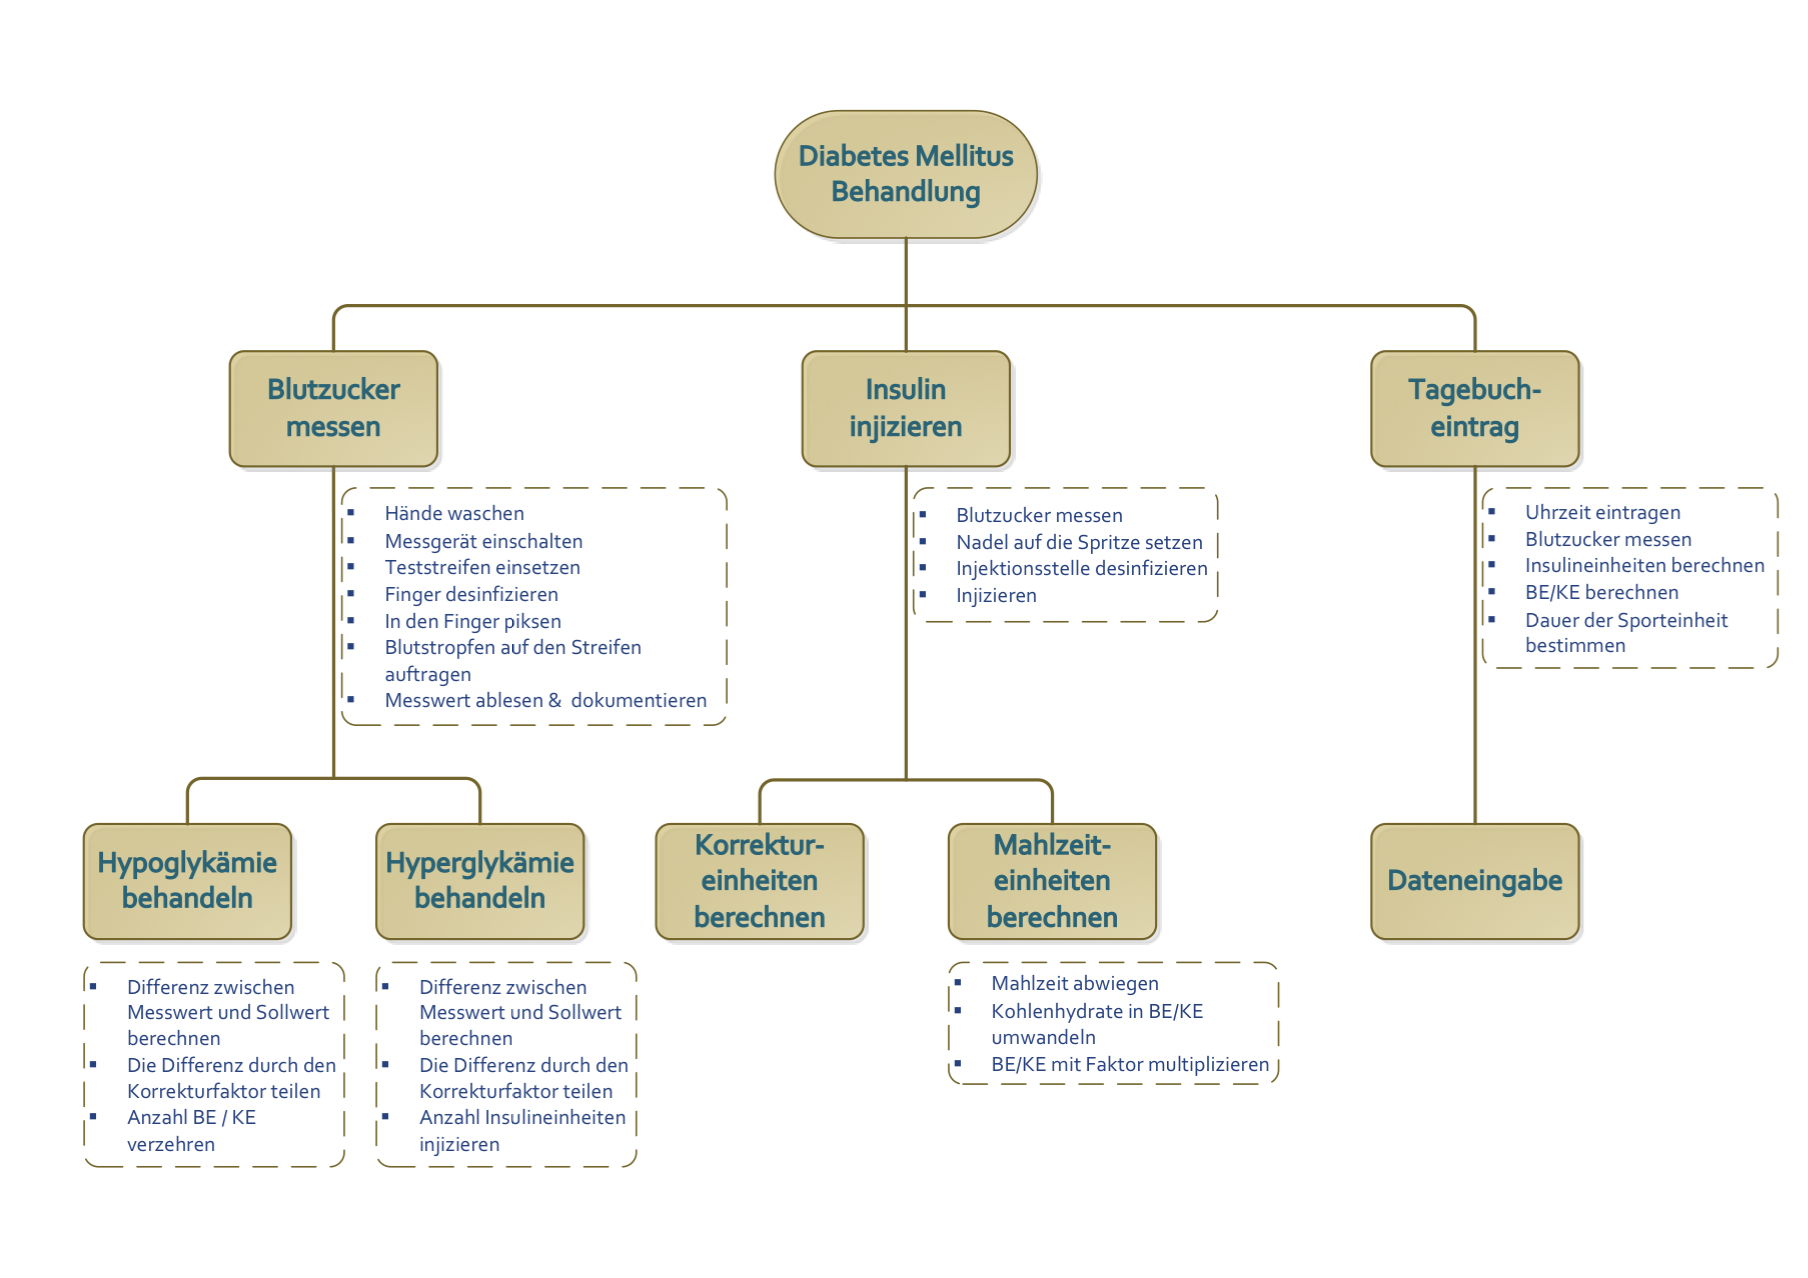
\includegraphics[width=1.0\textwidth]{images/taskOrganizationModel.png}}
 	\captionsetup{justification=centering}
 	\caption{Task Organization Model}
 	\label{img:taskorganizationmodel}
 \end{figure}
 \subsection{Concrete Use Cases (CUC)}
 \paragraph{CUC 01 - Benutzerprofil anlegen}
  \begin{center}
 	\begin{longtable}[H]{|p{6cm}|p{6cm}|}
 		\hline
 		\textbf{User action} & \textbf{System response}\\
 		\hline
 		Der Benutzer möchte ein neues Benutzerprofil anlegen.& Das System präsentiert die Optionen „Anmelden“ und „Registrieren“.\\
 		\hline
 		Der Benutzer wählt die Option „Registrieren“. &  Das System präsentiert ein Formular mit den notwendigen Spezifikationskriterien eines Benutzerprofils.\\
 		\hline
 		Der Benutzer spezifiziert seinen Vornamen, Nachnamen, Geburtsdatum, Geschlecht, Körpergröße, Körpergewicht, Benutzername, 
 		E-Mail-Adresse, Passwort, Behandlungsart, BE/KE-Faktor, Korrekturfaktor, Aktivitäten. & Das System 	füllt das Formular mit den Eingaben.\\
 		\hline
 		Der Benutzer speichert seine Angabe über die Option „Speicher“. & Das System speichert das Benutzerprofil.\\
 		\hline
 		\captionsetup{justification=centering}
 		\caption{CUC 01 - Benutzerprofil anlegen}
 		\label{tab:Persona Use Cases 1}
 	\end{longtable}
 \end{center}
\paragraph{CUC 02 - Benutzerprofil bearbeiten}
\begin{center}
	\begin{longtable}[H]{|p{6cm}|p{6cm}|}
		\hline
		\textbf{User action} & \textbf{System response}\\
		\hline
		Der Benutzer möchte sein bestehendes Benutzerprofil bearbeiten. & Das System präsentiert die Option „Profil bearbeiten“.\\
		\hline
		Der Benutzer wählt die Option „Profil bearbeiten“. &  Das System präsentiert ein Formular und die Spezifikationskriterien des Benutzerprofils.\\
		\hline
		Der Benutzer verändert die Spezifikationskriterien des Benutzerprofils. & Das System nimmt Änderung in das Formular auf.\\
		\hline
		Der Benutzer speichert seine Angabe über die Option „Speicher“. & Das System speichert das Benutzerprofil.\\
		\hline
		\captionsetup{justification=centering}
		\caption{CUC 02 - Benutzerprofil bearbeiten}
		\label{tab:Persona Use Cases 2}
	\end{longtable}
\end{center}
\paragraph{CUC 03 - Diabetes-Ereignis anlegen}
\begin{center}
	\begin{longtable}[H]{|p{6cm}|p{6cm}|}
		\hline
		\textbf{User action} & \textbf{System response}\\
		\hline
		Der Benutzer möchte ein neues Diabetes-Ereignis hinzufügen. & Das System präsentiert die Option „Diabetes“, „Mahlzeit“, „Aktivität“\ und „Beitrag“\\
		\hline
		Der Benutzer wählt die Option „Diabetes“. &  Das System präsentiert ein Formular und die Spezifikationskriterien des Ereignisses mit dem aktuellem Datum und der aktuellen Uhrzeit.\\
		\hline
		Der Benutzer spezifiziert seinen Blutzuckerwert. & Das System nimmt die Eingabe im Formularfeld „Blutzuckerwert" auf und präsentiert im Formularfeld „Korrekturinsulin“ die berechneten Insulineinheiten und im Formularfeld „BE“/„KE“ die berechneten BE/KE.\\
		\hline
		Der Benutzer speichert seine Angabe über die Option „Speicher“. & Das System speichert das Ereignis.\\
		\hline
		\captionsetup{justification=centering}
		\caption{CUC 03 - Diabetes-Ereignis anlegen}
		\label{tab:Persona Use Cases 3}
	\end{longtable}
\end{center}
\paragraph{CUC 04 - Mahlzeit anlegen}
\begin{center}
	\begin{longtable}[H]{|p{6cm}|p{6cm}|}
		\hline
		\textbf{User action} & \textbf{System response}\\
		\hline
		Der Benutzer möchte ein neues Malzeit-Ereignis hinzufügen. & Das System präsentiert die Option „Diabetes“, „Mahlzeit“, „Aktivität“\ und „Beitrag“\\
		\hline
		Der Benutzer wählt die Option „Mahlzeit“. &  Das System präsentiert ein Formular und die Spezifikationskriterien des Ereignisses mit dem aktuellem Datum und der aktuellen Uhrzeit.\\
		\hline
		Der Benutzer spezifiziert die Mahlzeit. & Das System präsentiert eine Auswahlmöglichkeit passender Mahlzeiten.\\
		\hline
		Der Benutzer spezifiziert seine Auwahl. & Das System nimmt die Mahlzeit im Formularfeld „Mahlzeit“ auf.\\
		\hline
		Der Benutzer spezifiziert die Menge der Mahlzeit. & Das System nimmt die Menge im Formularfeld „Menge“ auf, berechnet die BE/KE und Insulineinheiten und präsentiert diese.\\
		\hline
		Der Benutzer speichert seine Angabe über die Option „Speicher“. & Das System speichert das Ereignis.\\
		\hline
		\captionsetup{justification=centering}
		\caption{CUC 04 - Mahlzeit anlegen}
		\label{tab:Persona Use Cases 4}
	\end{longtable}
\end{center}
\paragraph{CUC 05 - Aktivität anlegen}
\begin{center}
	\begin{longtable}[H]{|p{6cm}|p{6cm}|}
		\hline
		\textbf{User action} & \textbf{System response}\\
		\hline
		Der Benutzer möchte ein neues Aktivität-Ereignis hinzufügen. & Das System präsentiert die Option „Diabetes“, „Mahlzeit“, „Aktivität“\ und „Beitrag“\\
		\hline
		Der Benutzer wählt die Option „Aktivität“. &  Das System präsentiert ein Formular und die Spezifikationskriterien des Ereignisses mit dem aktuellem Datum und der aktuellen Uhrzeit.\\
		\hline
		Der Benutzer spezifiziert die Aktivität. & Das System präsentiert eine Auswahlmöglichkeit passender Aktivitäten.\\
		\hline
		Der Benutzer spezifiziert seine Auwahl. & Das System nimmt die Aktivität im Formularfeld „Aktivität“ auf.\\
		\hline
		Der Benutzer spezifiziert die Dauer der Aktivität. & Das System nimmt die Dauer im Formularfeld „Dauer“ auf, berechnet die Kalorien und präsentiert diese.\\
		\hline
		Der Benutzer speichert seine Angabe über die Option „Speicher“. & Das System speichert das Ereignis.\\
		\hline
		\captionsetup{justification=centering}
		\caption{CUC 05 - Aktivität anlegen}
		\label{tab:Persona Use Cases 5}
	\end{longtable}
\end{center}
\paragraph{CUC 06 - Beitrag teilen}
\begin{center}
\begin{longtable}[H]{|p{6cm}|p{6cm}|}
	\hline
	\textbf{User action} & \textbf{System response}\\
	\hline
	Der Benutzer möchte ein neuen Beitrag hinzufügen. & Das System präsentiert die Option „Diabetes“, „Mahlzeit“, „Aktivität“\ und „Beitrag“\\
	\hline
	Der Benutzer wählt die Option „Aktivität“. &  Das System präsentiert ein Eingabefeld für den Inhalt des Beitrages.\\
	\hline
	Der Benutzer spezifiziert den Inhalt des Beitrages. & Das System nimmt die Eingabe auf.\\
	\hline
	Der Benutzer speichert seine Angabe über die Option „Teilen“. & Das System speichert den Beitrag.\\
	\hline
	\captionsetup{justification=centering}
	\caption{CUC 06 - Beitrag teilen}
	\label{tab:Persona Use Cases 6}
\end{longtable}
\end{center}
	\newpage
	
	\section{Design}
	Bestandteil der zweiten fundermentalen Phase des Usability Engineering Lifecycle ist das Design, in dem zunächst das Task Organzation Model anhand der Concrete Use Cases überarbeitet und folglich Design Standards bestimmt werden, um abschließend die Screens des User Interfaces zu entwerfen. 
	\subsection{Reengineered Task Organization Model}
Das Reengineered Task Organization Model repräsentiert die Arbeit der Benutzer mithilfe des zu entwicklende System. Die Abbildung \ref{img:reengineeredTaskOrganizationModel}: \nameref{img:reengineeredTaskOrganizationModel} beschreibt den Prozess der Arbeit des Diabetikers mit dem System anhand der Concrete Use Cases aus der Aufgebenmodellierung und ergänzt das Task Organization Model. Alle Erkenntisse aus der Aufgabenmodellierung fließen zunächst in das Reengineered Task Organization Model und folglich auch in das Design der Screens ein.
\begin{figure}[H]
	\centering
	\setlength{\fboxsep}{1pt}
	\setlength{\fboxrule}{1pt}
	\fbox{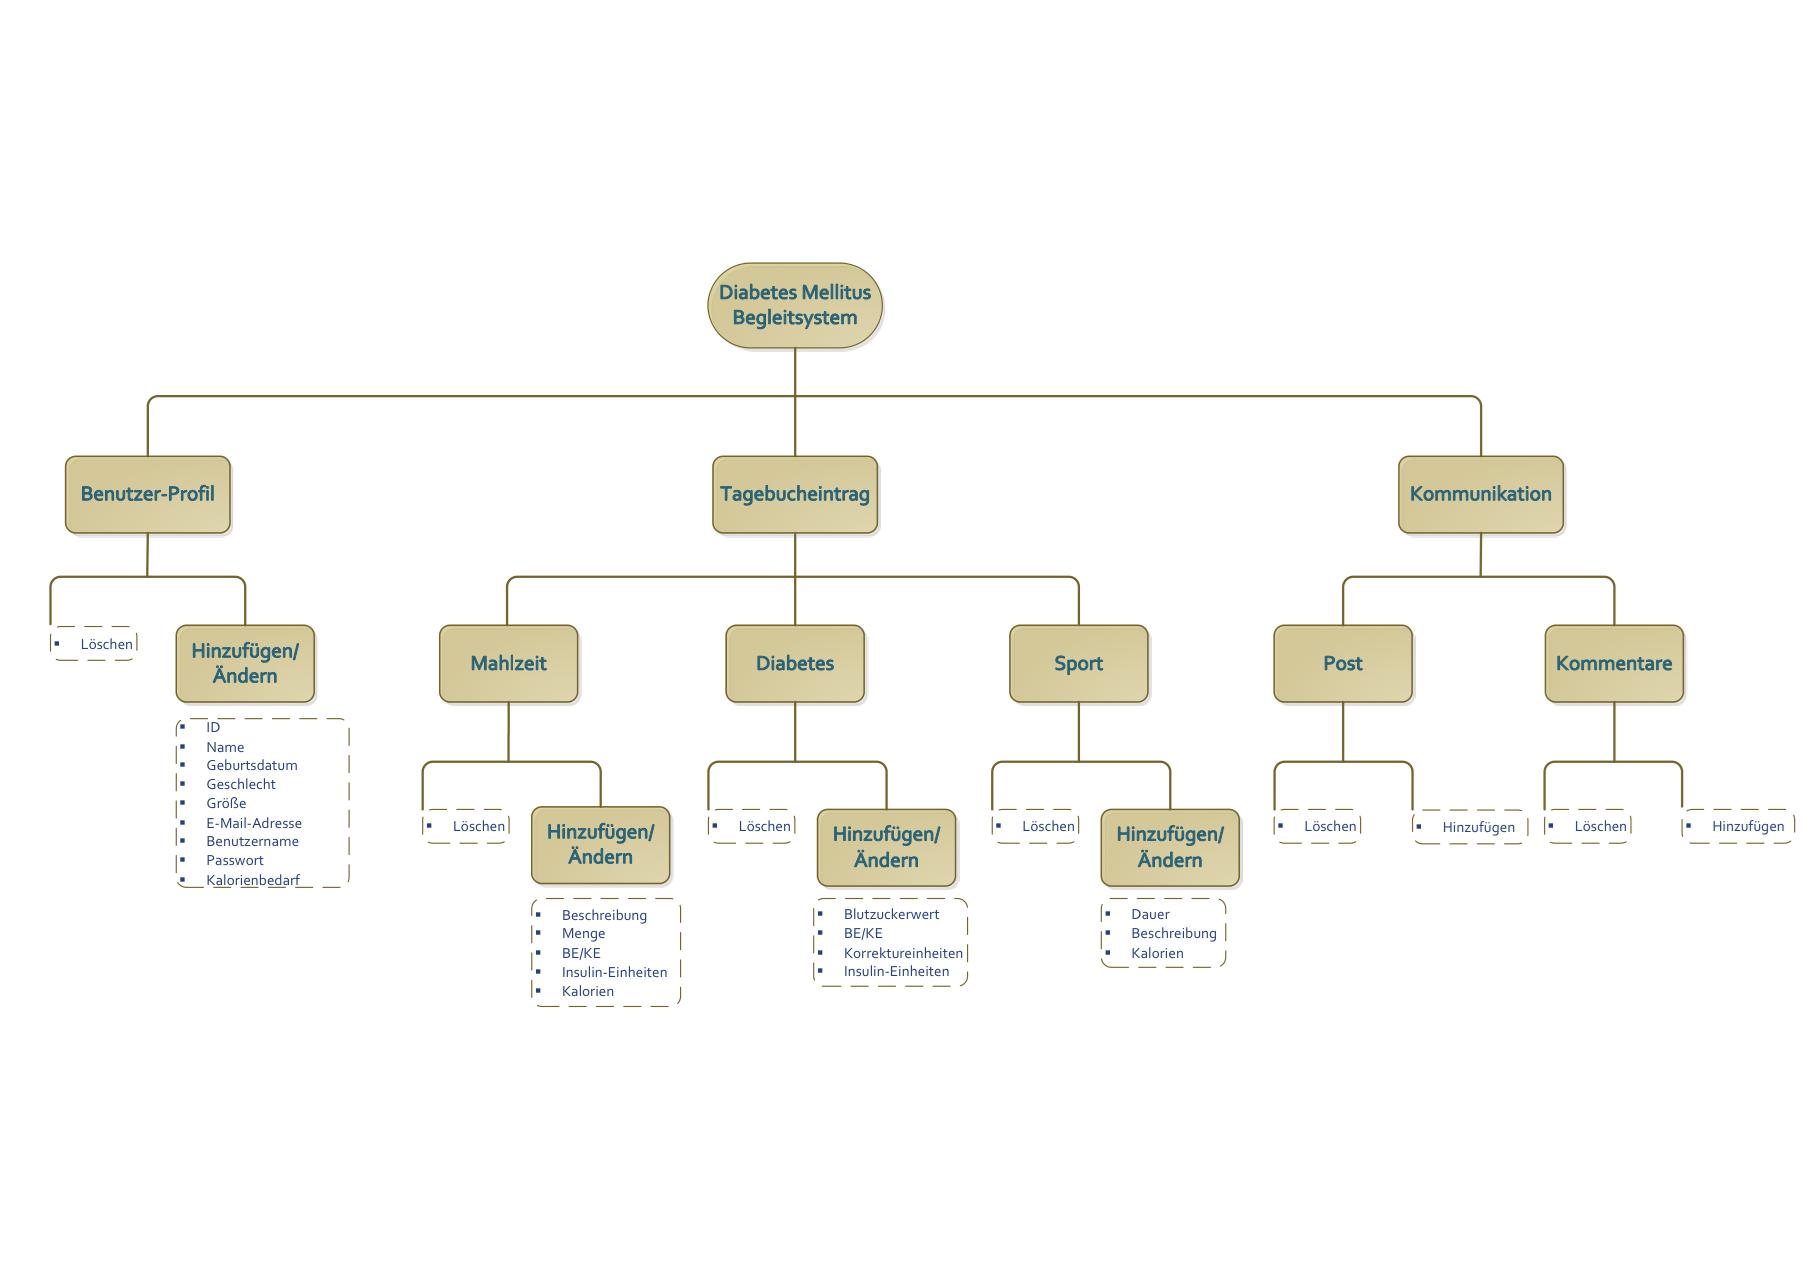
\includegraphics[width=1.0\textwidth]{images/reengineeredTaskOrganizationModel.png}}
	\captionsetup{justification=centering}
	\caption{Reengineered Task Organization Model}
	\label{img:reengineeredTaskOrganizationModel}
\end{figure}
\subsection{Conceptual Model (CM) Design}
Im Concetpual Model Design werden erste Screens für das zu entwickelnde System designt. Die ersten groben Entwürfe sollen den Navigationspfad und die Haupt-Screens identifizieren und anhand dessen erste Regeln für das finale Design des Interfaces festlegen. Ziel ist hier jedoch nicht ein detailreiches Interface Design zu bestimmen. Dieses Design muss zunächst in den kommenden Designaufgaben entwickelt werden.\\
Nach Mayhew \cite{MD} muss zunächst bestimmt werden, ob es sich bei dem Conceputal Model Design um ein product- oder process-oriented model handelt. Da es in dem zu entwickelnde System keine Arbeitsprodukte, welche vom Benutzer individuell erstellt oder bearbeitet werden. In diesem System sollen die Arbeitsprozesse von Diabetikern unterstützt werden. Auf Informationen wie die Nährwerte von Lebensmitteln haben alle Benutzer Zugriff, können abgerufen und in ihrem Tagebuch gespeichert werden. Aufgrund dessen handelt es sich in diesem Fall um ein process-oriented model.\\
In nächsten Schritt sind die Prozesse des process-oriented model zu identifizieren. Bei einem process-oriented model definiert das \nameref{img:reengineeredTaskOrganizationModel} auf Seite \pageref{img:reengineeredTaskOrganizationModel} die (Unter-)Prozesse des Systems und aus diesem lässt sich folgende Aufgabenhierarchie ableiten:\\
Benutzer\newline
\noindent\hspace*{10mm}Benutzer hinzufügen\newline
\noindent\hspace*{10mm}Benutzer bearbeiten\newline
\noindent\hspace*{10mm}Benutzer löschen\newline
Tagebuch\newline
\noindent\hspace*{10mm}Blutzuckerwert\newline
\noindent\hspace*{20mm}Blutzuckerwert hinzufügen\newline
\noindent\hspace*{20mm}Blutzuckerwert bearbeiten\newline
\noindent\hspace*{20mm}Blutzuckerwert löschen\newline
\noindent\hspace*{10mm}Mahlzeit\newline
\noindent\hspace*{20mm}Mahlzeit hinzufügen\newline
\noindent\hspace*{20mm}Mahlzeit bearbeiten\newline 
\noindent\hspace*{20mm}Mahlzeit löschen\newline
\noindent\hspace*{10mm}Aktivität\newline
\noindent\hspace*{20mm}Aktivität hinzufügen\newline
\noindent\hspace*{20mm}Aktivität bearbeiten\newline
\noindent\hspace*{20mm}Aktivität löschen\newline
Kommunikation\newline
\noindent\hspace*{10mm}Beitrag\newline
\noindent\hspace*{20mm}Beitrag hinzufügen\newline
\noindent\hspace*{20mm}Beitrag löschen\newline
\noindent\hspace*{10mm}Kommentar\newline
\noindent\hspace*{20mm}Kommentar hinzufügen\newline
\noindent\hspace*{20mm}Komentar löschen\\
Um nun die Darstellungregeln für die Prozesse zu gestalten wird eine Bottom-Navigation-Bar verwendet. Die Navigation könnte wie in Abbildung \ref{img:navigationbar}: \nameref{img:navigationbar} dargestellt werden. \newline
Für eine Bottom-Navigation-Bar wurde sich entschieden, um den Benutzer Kontrolle über das System und eine gewisse Freiheit zu gewährleisten. So ermöglicht das System dem Benutzer bei versehentlicher Auswahl einer Navigation einen deutlich gekennzeichneten „Notausgang“, indem der Benutzer lediglich durch die Bottom-Navigation den unerwünschten Systemzustand verlässt, ohne einen erweiterten Dialog durchlaufen zu müssen.
\begin{figure}[H]
	\centering
	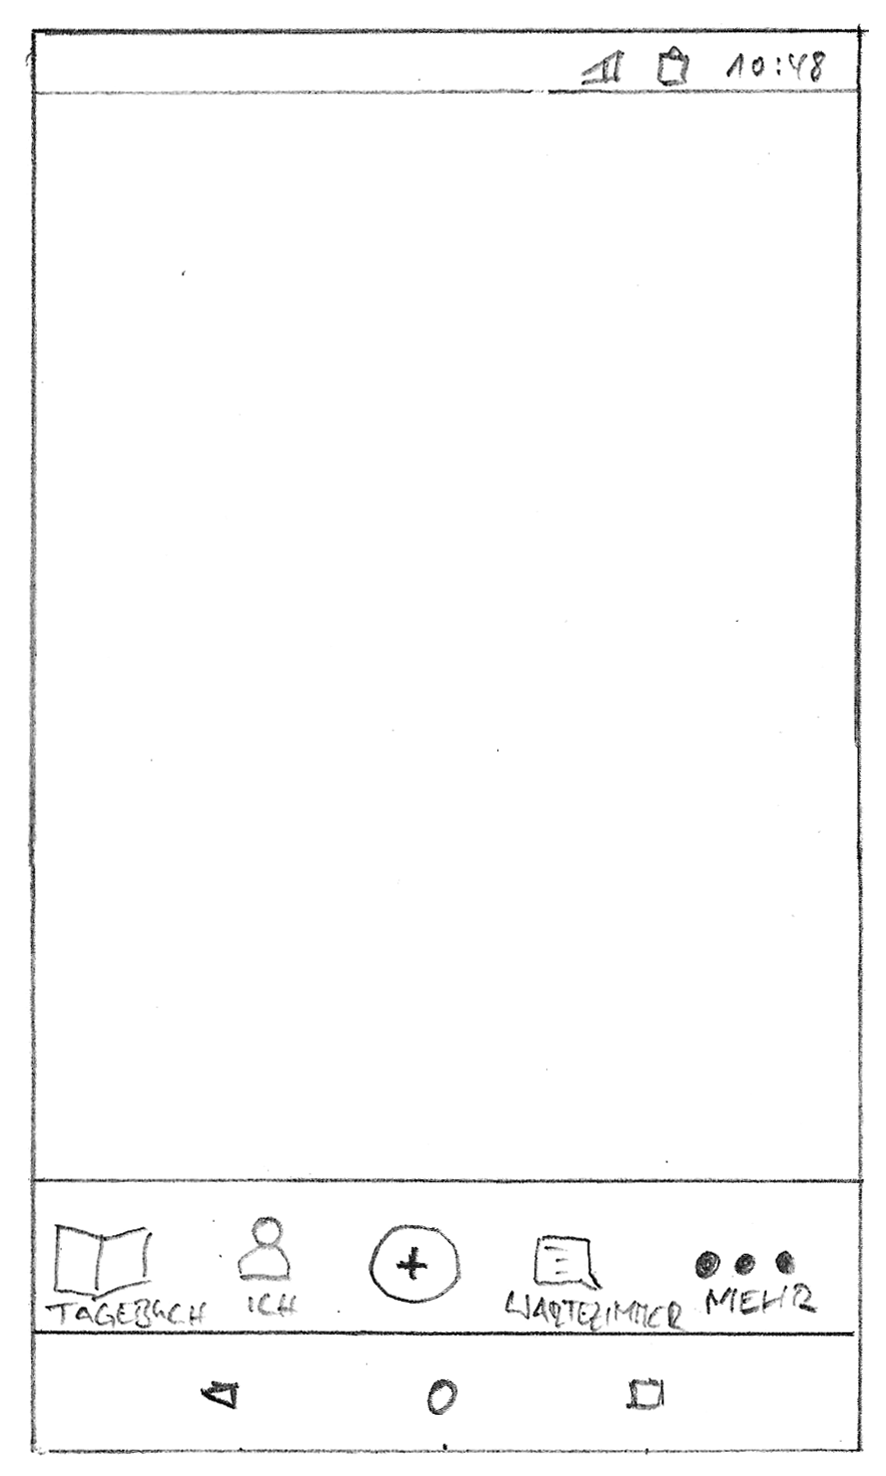
\includegraphics[width=0.35\textwidth]{images/navigationbar.png}
	\captionsetup{justification=centering}
	\caption{Bottom-Navigation-Bar}
	\label{img:navigationbar}
\end{figure}
Unter dem Navigationspfad „Tagebuch“ (Abbildung \ref{img:tagebuchscreen}: \nameref{img:tagebuchscreen})sind Blutzuckerwerte, Mahlzeiten und Aktivitäten anzulegen, zu bearbeiten, einzusehen und zu löschen. Unter „Ich“ (Abbildung \ref{img:ichscreen}: \nameref{img:ichscreen}) und „Mehr“ (Abbildung \ref{img:mehrscreen}: \nameref{img:mehrscreen}) können Benutzerkonten eingesehen, bearbeitet und gelöscht werden und im „Wartezimmer“ (Abbildung \ref{img:wartezimmerscreen}: \nameref{img:wartezimmerscreen}) sind Beiträge und Kommentage einzusehen, hinzuzufügen und zu löschen. Das Plus-Icon ermöglich zusätzlich das hinzufügen von Blutzuckerwerten, Mahlzeiten, Aktivitäten und Beiträge. So könnten die Screens folgendermaßen dargestellt werden. 
\begin{figure}[H]
	\centering
	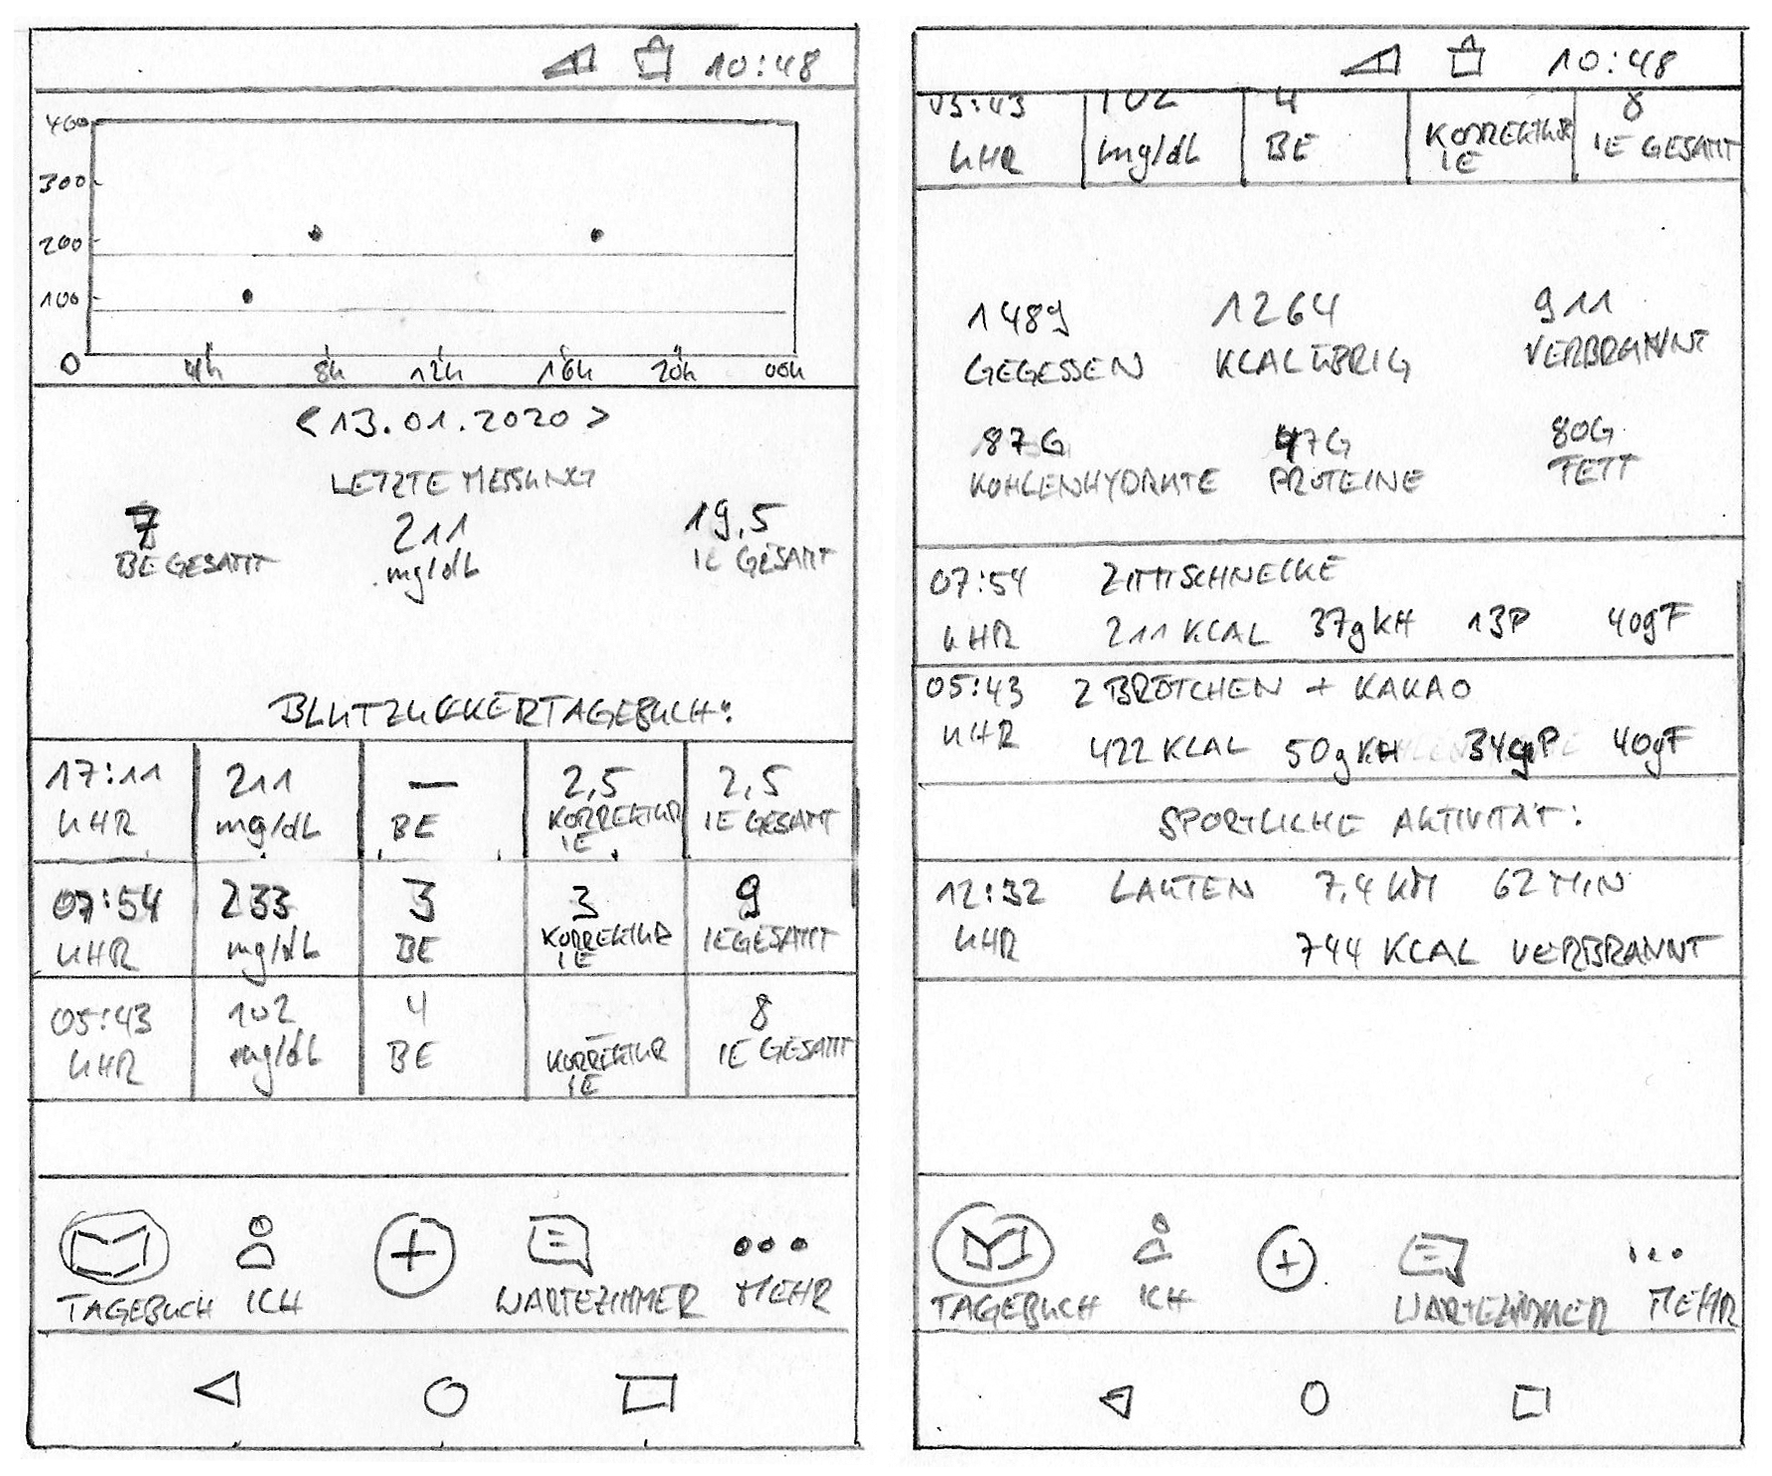
\includegraphics[width=0.7\textwidth]{images/tagebuchscreen.png}
	\captionsetup{justification=centering}
	\caption{Tagebuch-Screen}
	\label{img:tagebuchscreen}
\end{figure}
\begin{figure}[H]
	\centering
	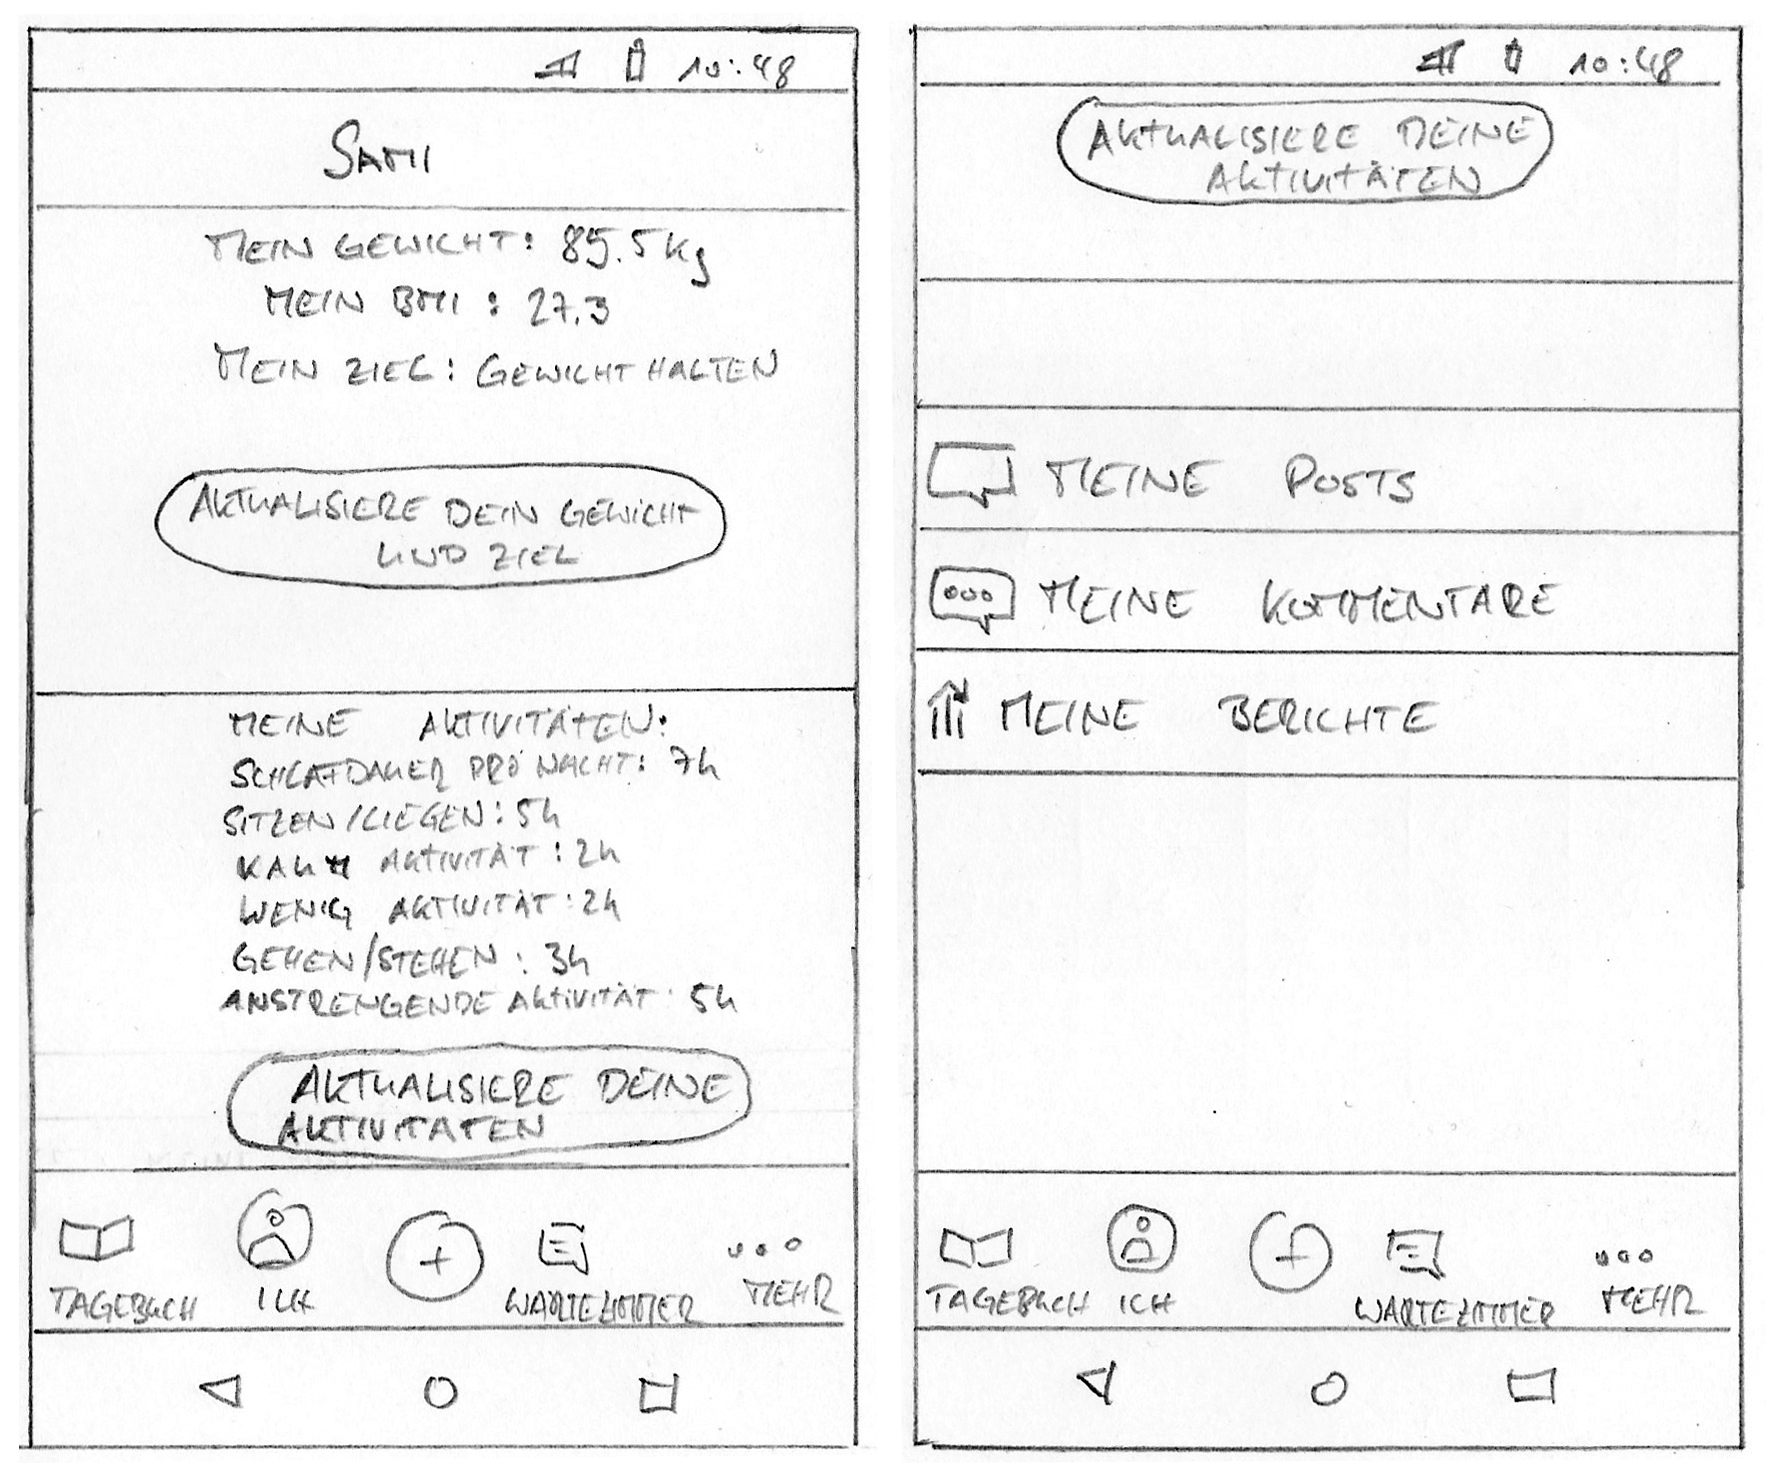
\includegraphics[width=0.7\textwidth]{images/ichscreen.png}
	\captionsetup{justification=centering}
	\caption{Ich-Screen}
	\label{img:ichscreen}
\end{figure}
\begin{figure}[H]
	\centering
	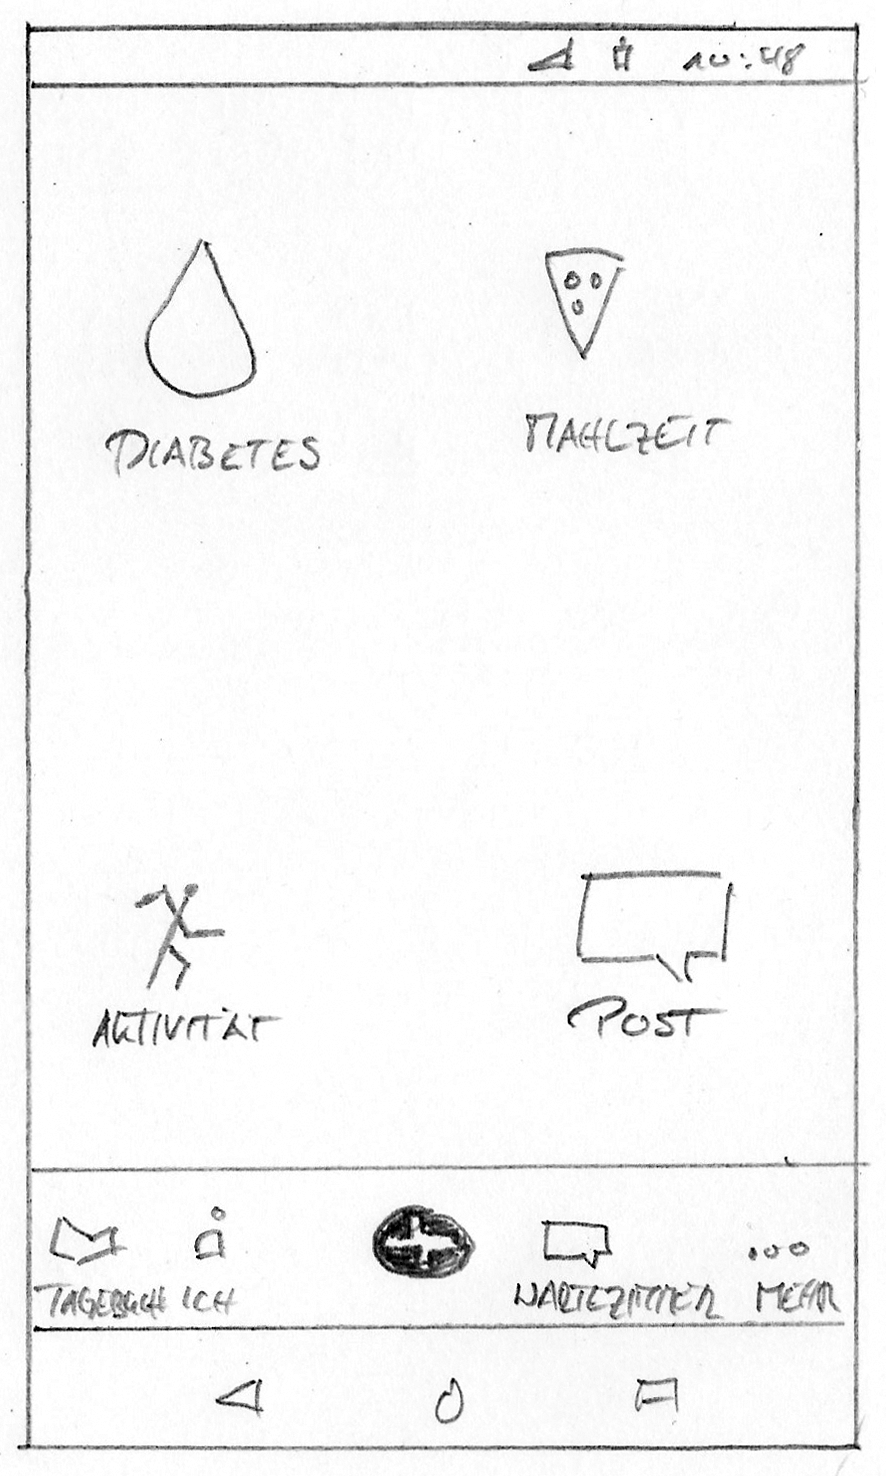
\includegraphics[width=0.35\textwidth]{images/addscreen.png}
	\captionsetup{justification=centering}
	\caption{Add-Screen}
	\label{img:addscreen}
\end{figure}
\begin{figure}[H]
	\centering
	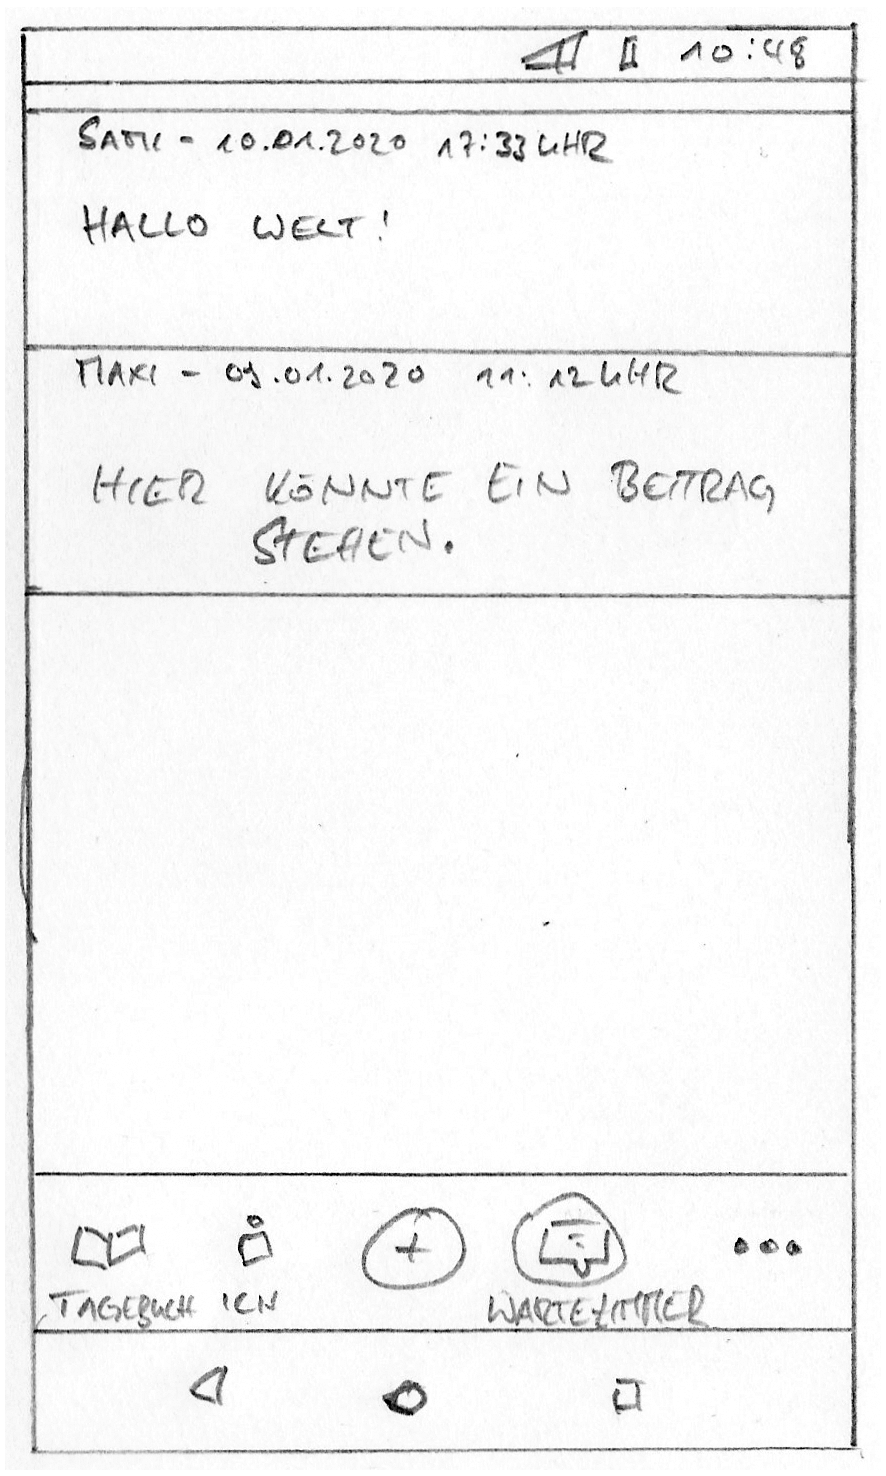
\includegraphics[width=0.35\textwidth]{images/wartezimmerscreen.png}
	\captionsetup{justification=centering}
	\caption{Wartezimmer-Screen}
	\label{img:wartezimmerscreen}
\end{figure}
\begin{figure}[H]
	\centering
	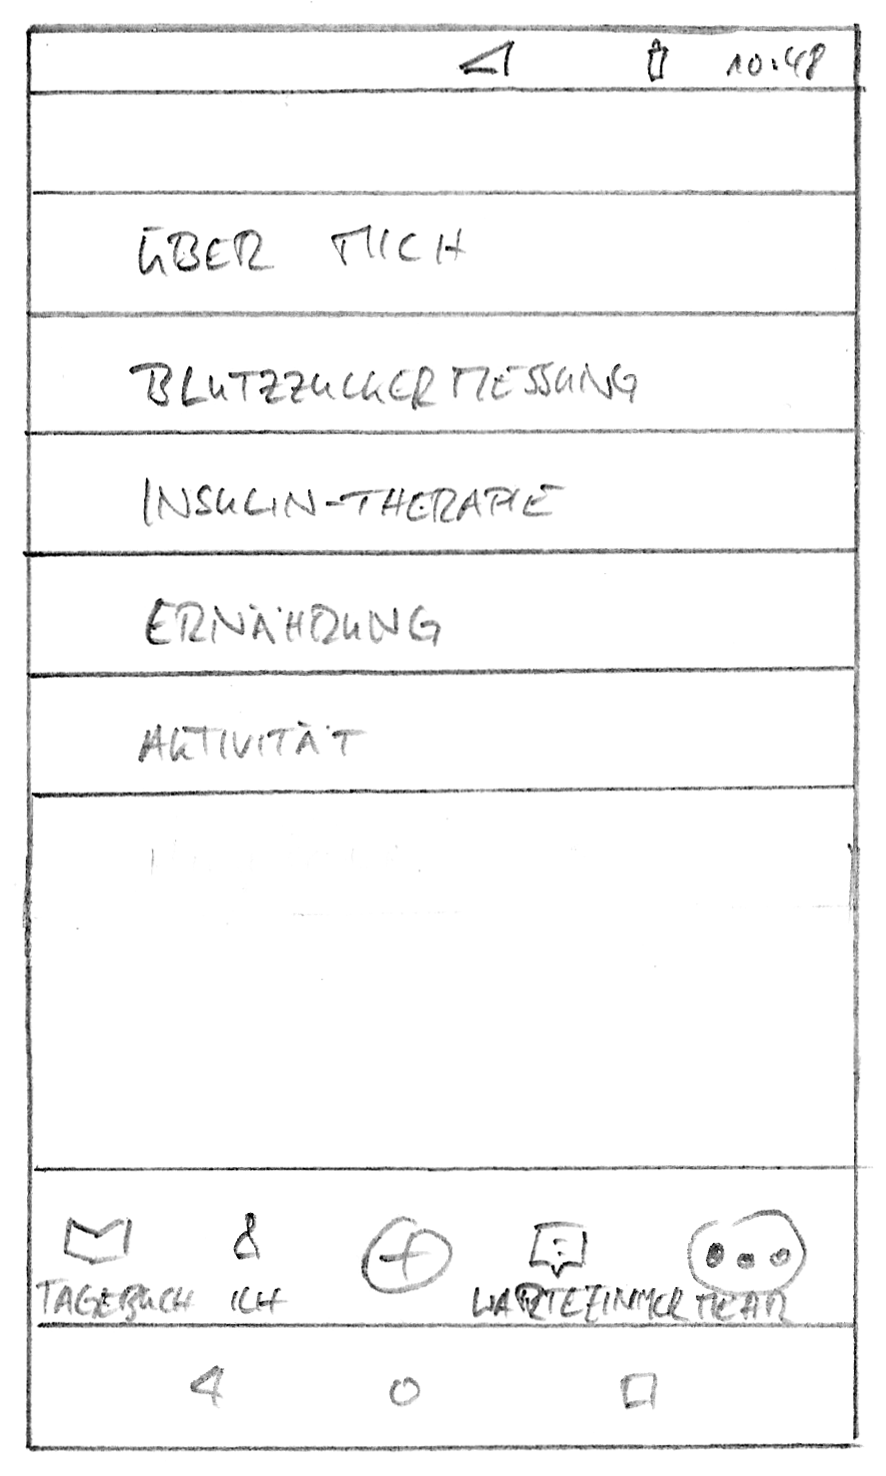
\includegraphics[width=0.35\textwidth]{images/mehrscreen.png}
	\captionsetup{justification=centering}
	\caption{Mehr-Screen}
	\label{img:mehrscreen}
\end{figure}
Die Begriffswahl für „Tagebuch“ (Abbildung \ref{img:tagebuchscreen}: \nameref{img:tagebuchscreen}) ensteht aus der Domäne, das Diabetiker „Tagebucheinträge“ verfassen.  „Ich“ (Abbildung \ref{img:ichscreen}: \nameref{img:ichscreen}) repräsentiert benutzerbezogene Daten und „Wartezimmer“ (Abbildung \ref{img:wartezimmerscreen}: \nameref{img:wartezimmerscreen} ist eine metaphorische Bezeichnung für eine Treffpunkt verschiedener Benutzer. Unter „Mehr“ (Abbildung \ref{img:mehrscreen}: \nameref{img:mehrscreen}) sind wiederum benutzerbezogene Einstellungen zu bearbeiten. Durch die verschiedenen Navigationspfade soll der Benutzer durch stets angemessene Informationen innerhaln angemessener Zeit auf dem Laufenden gehalten werden.\\
Nach dem Conceputal Model Design folgt das Conceptual Model Mock-Up und die Iterative Conceptual Model Evaluation, in denen die ersten Entwürfe eines Designs mit Stift und Papier erstellt  und anhand von Probanden evaluiert werden. Da allerdings gibt der begrenzte Zeitrahmen diese zwei Arbeitschritte nicht her, wodurch die Abbildungen als Mock-Up dienen und eine Evaluation nicht durchgeführt werden kann. Folglich werden Screen Design Standards festgelegt und anhand dessen ein Style Guide erstellt.
\subsection{Screen Design Standards (SDS)}
Mithilfe der aus der Benutzer- und Aufgabenmodellierung stammenden Erkenntisse und dem Conceptual Model Design werden systemspezifische Standards und Konventionen für alle Aspekte des detaillierten Screen-Designs entwickelt. Dazu dienen die Screen Design Standards als Grundlage der Usability auf dem gesamten User Interface. Das zu entwickelnde System soll folgende Control und Dialog Box Standars aufweisen:\\
\centerline{\textbf{Control Standards}}
\begin{center}
	\begin{longtable}[H]{p{8cm}p{6cm}}
		\textbf{Menu Contents} & \textbf{Control}\\
		\toprule
		Navigational actions & Push icons\\
		Entering numbers & EditText with number to choose/Seekbar\\
		Entering decimal numbers &  EditText with decimal number to choose/Seekbar\\
		Entering text & EditText with letters to choose\\
		Choose date & DatePickerDialog\\
		Choose time & TimePickerDialog\\
		Variable list & Spinner\\
		\bottomrule
		\captionsetup{justification=centering}
		\caption{Control Standards}
		\label{tab:controlstandars}
	\end{longtable}
\end{center}
\centerline{\textbf{Dialog Box Standards}}
\begin{itemize}
	\item Always use blue as dialog box background color 
	\item Match title to the menu bar selection that brought it up, left hustified in the title bar
	\item Create vertical groups of logically related fields
	\item Within field groups, center-align captions, center-align fields, try to minimize white space between captions and fields, use first-letter caps for all main words in captions
\end{itemize}
Unter berücksichtigung dieser Standards könnten Dialog Boxes aussehen wie in Abbildung \ref{img:dialogbox}: \nameref{img:dialogbox}.
\begin{figure}[H]
	\centering
	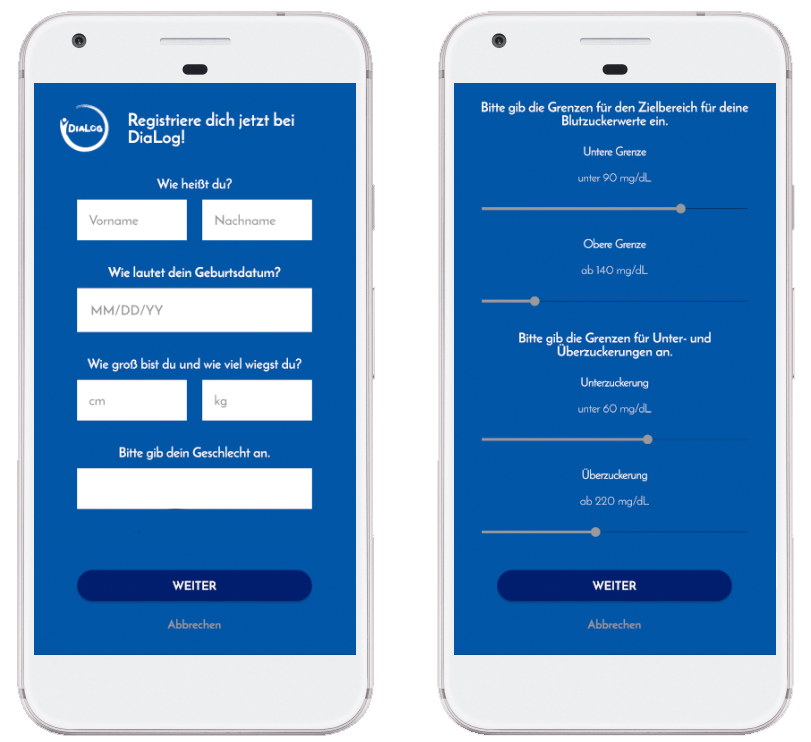
\includegraphics[width=0.7\textwidth]{images/DialogBox.png}
	\captionsetup{justification=centering}
	\caption{Dialog Boxes}
	\label{img:dialogbox}
\end{figure}
Hinzu kommen folgende Standards:
\begin{itemize}
	\item Use group boxes, embed all-caps titles in upper center of group box
	\item Order groups left to right, top to bottom according to natural order or expected frequency of use
	\item Always place the Weiter push button in the middle at the bottom and above the Abbrechen push button, all push buttons evenly apart
	\item Background color for fields:\newline
		\noindent\hspace*{30mm}Read-only - blue \newline
		\noindent\hspace*{30mm}Required - white \newline
		\noindent\hspace*{30mm}Optional - gray 
\end{itemize}

\subsection{Style Guide}
Um nun die Screen Design Standards zu vervollständigen, wird ein Style Guide erstellt. Dieser fügt dem User Interface folgende Kriterien hinzu:\\
	\newpage
	
	\section{Systemdokumentation}
	\subsection{Systemarchitektur}
Das Reengineered Task Organization Model repräsentiert die Arbeit der Benutzer mithilfe des zu entwicklende System. Die Abbildung \ref{img:reengineeredTaskOrganizationModel}: \nameref{img:reengineeredTaskOrganizationModel} beschreibt den Prozess der Arbeit des Diabetikers mit dem System anhand der Concrete Use Cases aus der Aufgebenmodellierung und ergänzt das Task Organization Model.
\begin{figure}[H]
	\centering
	\setlength{\fboxsep}{1pt}
	\setlength{\fboxrule}{1pt}
	\fbox{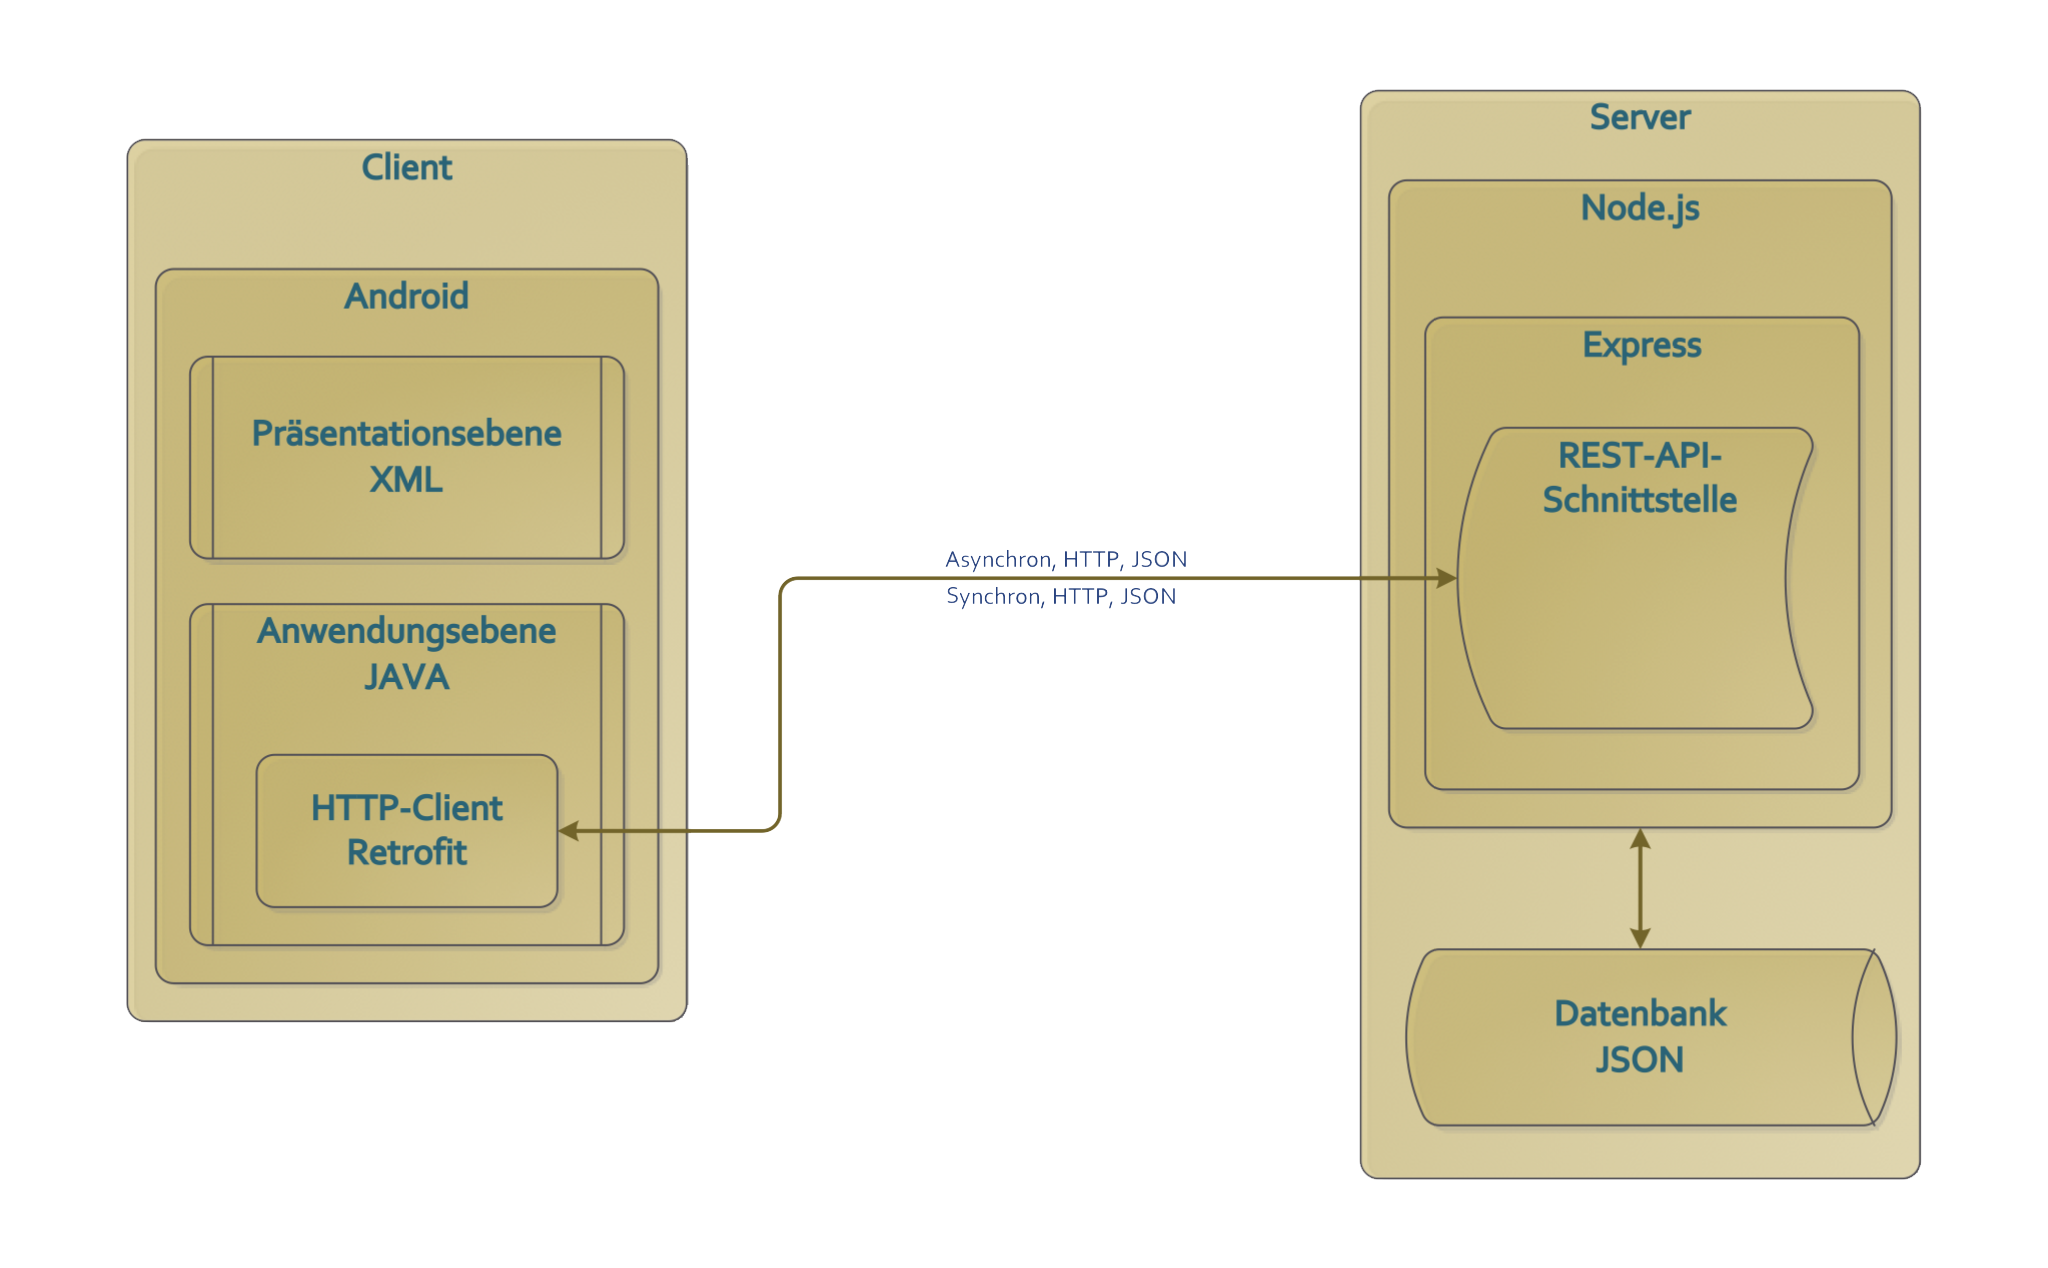
\includegraphics[width=1.0\textwidth]{images/systemarchitektur.png}}
	\captionsetup{justification=centering}
	\caption{Systemarchitektur}
	\label{img:Systemarchitektur}
\end{figure}
	\newpage
	
	
	
	\newpage
	
	\begin{thebibliography}{1}\markboth{Literaturverzeichnis}{Literaturverzeichnis}\addcontentsline{toc}{section}{Literaturverzeichnis}
		
		\bibitem{AD}
		Abbott Diabetes Care Inc.:
		Produkte zur Grukosemessung - Willkommen in der FreesStyle Familie, letzter Aufruf: 02.12.19 von:
		https://freestyle.de/produkte/	
		
		\bibitem{CL}
		Constantine, Larry L.; Lochwood, Lucy A.D.: 
		Software for Use, 
		Reading, Massachusetts: Addison Wesley,
		1999.
		
		\bibitem{DDG}
		Deutsche Diabetes Gesellschaft (DDG); diabetesDE - Deutsche Diabetes-Hilfe:
		Deutscher Gesundheitsbericht, Diabetes 2019 - Die Bestandsaufnahme, 
		Mainz: Verlag Kirchheim + Co. GmbH,
		2019.
		
		\bibitem{D}
		Dexcom:
		Das neue Dexcom G6® - Real-Time-CGM-System (rtCGM). Entdecken Sie die Vorteile des Dexcom G6., letzter Aufruf: 01.12.19, von: https://www.dexcom.com/de-DE/de-dexcom-g6-cgm-system
		
		\bibitem{DC}
		DiabetesConnect:
		Deine Dokumentation - Einfach und schnell, letzter Aufruf: 01.12.19, von: http://www.diabetesconnect.de
		
		\bibitem{DiRECT}
		Diabetes Remission Clinical Trial (DiRECT):
		Two-year results of the randomised Diabetes Remission Clinical Trial (DiRECT), veröffentlicht am 07.02.2019, \newline
		letzter Aufruf: 30.11.2019, von: https://www.directclinicaltrial.org.uk/Pubfiles/Final\newline\%20accepted\%20draft,\%20prior\%20to\%20editing\%20and\%20corrections.pdf
		
		\bibitem{DED}
		Die Ernährungs-Docs | NDR:
		Typ-2-Diabetes: Wie man vom Insulin wieder wegkommt, \newline
		https://www.youtube.com/watch?v=CTR7KQog5kU\newline
		2017
		
		\bibitem{HG}
		Prof. Dr. Hartmann, Gerhard: 
		Vorlesungsbegleitende Materialien zum Modul Mensch-Computer Interaktion, 
		2016.
		
		\bibitem{IDF}
		International Diabetes Federation (IDF): 
		IDF Diabetes Atlas, Eighth Edition 2017.
		
		\bibitem{JR}
		Jäckle, Renate: 
		Gut leben mit Typ-1-Diabetes, 7. Auflage
		München: Elsevier GmbH,
		2010.
		
		\bibitem{JS}
		Journal Stuttgart - Regio TV: 
		Leben mit Diabetes | 15.08.2018, \newline
		https://www.youtube.com/watch?v=EqZEZyEz7sM \newline
		2018.
		
		\bibitem{KM}
		Karmasin, Matthias; Ribing, Rainer: 
		Die Gestaltung wissenschaftlicher Arbeit, 9. Auflage,
		Wien: facultas,
		2017.
		
		\bibitem{L}
		Lifesum: Gesund leben. Leicht gemacht., letzter Aufruf: 02.12.19, von: \newline https://lifesum.com/de/
		
		
		\bibitem{MD}
		Mayhew, Deborah J.: 
		The Usability Engineering Lifecycle - a pracititoner handbook for user interface design,
		San Francisco, California: Morgan Kaufmann,
		1999.
		
		\bibitem{MS}
		MySugr:
		mySugr Diabetes App - dein digitales Tagebuch, letzter Aufruf: 30.11.2019, von:	
		https://mysugr.com/de-de/diabetes-app
		
		\bibitem{ND}
		Nestlé Deutschland AG: 
		Kalorien mundgerecht, 13. Auflage, Frankfurt/Main: Umschau,
		2006.
		
		\bibitem{RP}
		Rechenberg, Peter: 
		Technisches Schreiben - (nicht nur) für Informatiker, 2. Auflage,
		München Wien: Carl Hansen Verlag,
		2003.
		
		\bibitem{SG}
		Schmeisl, Gerhard-W: 
		Schulungsbuch für Diabetiker, 6. Auflage, 
		München: Elsevier GmbH,
		2009.
		
		\bibitem{TA}
		Tanenbaum, Andrew; van Steen, Marten: 
		Verteilte Systeme - Grundlagen und Paradigmen,
		München: Pearson Studium
		2003.
		
	\end{thebibliography}
	\newpage
	\appendix
	\vspace*{\fill}
	\part*{Anhang}\markboth{Anhang}{Anhang}\addcontentsline{toc}{part}{Anhang}
	\setcounter{section}{0}% 
	\setcounter{subsection}{0}% 
	\setcounter{figure}{0}
	\renewcommand{\thesection}{\Alph{section}}
	\renewcommand\thefigure{\Alph{section}\arabic{figure}}
	\vfill
	\newpage
	
	
	
	\section{Themenfeld/-recherche}
	\label{section:Themenfeld}
	\subsection{Diabetes-Arten}
	Ein gesunder menschlicher Körper produziert in der Bauchspeicheldrüse ein Hormon, namens Insulin. Insulin sorgt für den Transport von in Zucker aus dem Blut in die Muskelzellen und wandelt diesen dort in Energie um. Metaphorisch kann man sich Organismus als Schlüssel-Schloss-Prinzip vorstellen. Insulin stellt dabei den Schlüssel da, welcher die Muskelzellen, das Schloss, für den Eingang des Zuckers öffnet. Es gibt verschiedene Arten des Diabetes mellitus. \\	
	Der Typ-1-Diabetes ist chronisch und tritt aufgrund eines Gendefektes auf. Bei diesem Gendefekt verwechseln die Antikörper des Immunsystems die Zellen der Bauchspeicheldrüse, welche Insulin produziert, mit einem Virus und zerstört diese vollständig. Diese Zellen können sich nach der Auslöschung nicht regenerieren, sodass keine Insulinproduktion mehr möglich ist. Somit kann der Zucker nicht in die Muskelzellen gelangen und das Blut beginnt zu übersäuern. Diese Art des Diabetes mellitus kann in jeder Altersstufe auftreten und der Gendefekt kann vorhanden sein, ohne ausgelöst zu werden. Dieser Gendefekt ist erblich bedingt.\\
	Bei dem Typ-2-Diabetes spricht man von einem sogenannten „Alters-Diabetes“, bei dem die Bauchspeicheldrüse noch Insulin produziert, jedoch die Muskelzellen insulinresistent sind. Die Muskelzellen sind durch das hohe Alter und einer schlechten Ernährung sowie einer begrenzten sportlichen Aktivität gestört. Stellt man sich dies als Schlüssel-Schloss-Prinzip dar, sind zwar Schlüssel, in Form des Insulins, vorhanden, jedoch sind die Schlösser, die Muskelzellen, verrostet. Auch hier kommt es zu einer Übersäuerung des Blutes. Der Typ-2-Diabetes ist nicht chronisch und die Muskelzellen können sich durch Umstellungen in der Ernährung und im Sport wieder regenerieren.\\
	Weitere bekannte Arten des Diabetes mellitus sind zum einen der Schwangerschaftsdiabetes und zum anderen der Typ-3c-Diabetes.\newline
	Schwangerschaftsdiabetes wird auch Gestationsdiabetes (Typ-4-Diabetes) genannt und durchschnittlich bei 4\% aller schwangeren Frauen diagnostiziert. Diese Art von Diabetes tritt meist nur während der Schwangerschaft auf. Er beginnt zwischen dem 4. Und 6. Schwangerschaftsmonat und endet kurz nach der Geburt. In dieser Phase entwickelt der Körper eine Zunahme des Insulinbedarfs. Zudem nimmt die Produktion von Insulin in der Bauchspeicheldrüse ab. Hormone wie Progesteron, Human Plazenta-Laktogen und Östriol, die von der Plazenta (Mutterkuchen) hergestellt werden tragen ebenfalls zur Verminderung der Insulinempfindlichkeit bei. Nur in seltenen Fällen hat der Schwangerschaftsdiabetes fatale Folgen für Mutter oder Kind.\\
	Der Typ-3c-Diabetes ist ein recht komplexer Typ. Hier gibt es unterschiedliche Ursachen für den Typ-3c-Diabetes, bei dem die Insulinproduktion in der Bauchspeicheldrüse gestört wird. In den meisten Fällen sorgt eine chronische Entzündung der Bauchspeicheldrüse für die Einstellung der Insulinproduktion. Ursachen für Entzündungen können ein dauerhaft hoher Alkoholkonsum oder ein erhöhter Calcium-Spiegel sein. In beiden Fällen tritt der Diabetes auf, wenn 90\% der Inselzellen in der Bauchspeicheldrüse ausgelöscht wurden.\newline
	Weitere Ursachen für die Erkrankung an dem Typ-3c-Diabetes können Verletzungen an der Bauchspeicheldrüse, durch beispielsweise Unfälle, oder auch notwendige Bauchspeicheldrüsenentfernung sein. Auch Krebs oder Tumore in der Bauchspeicheldrüse können die Insulinproduktion einschränken. Der Typ-3c-Diabtetes tritt nicht häufig auf und ist meist eine Nebenerkrankung bei viel schwerwiegenderen Erkrankungen der Bauchspeicheldrüse. \emph{[Schmeisl, Gerhard-W: Schulungsbuch für Diabetiker, 6. Auflage, München: Elsevier GmbH, 2009.]} 
	\subsection{Analoge Dokumentation}
	In Abbildung \ref{img:tagebuch}: \nameref{img:tagebuch} ist ein Bespiel der Dokumentation von Blutzuckerwerten eines Diabetikers an einem Tag zu sehen. Ein Diabetiker sollte jeden Tag mindestens viermal den Blutzucker messen und diesen auch dokumentieren.
	\begin{figure}[H]
		\centering
		\setlength{\fboxsep}{1pt}
		\setlength{\fboxrule}{1pt}
		\fbox{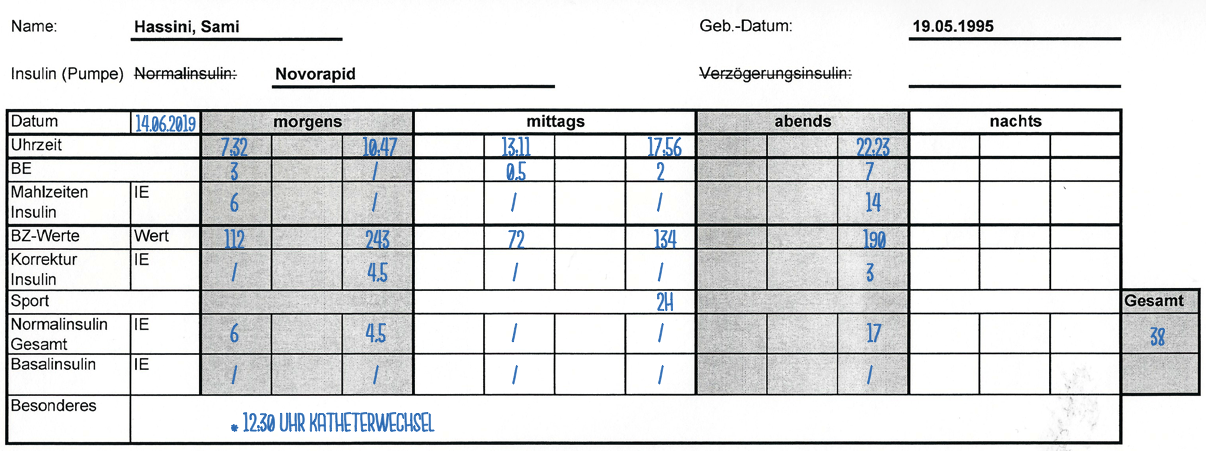
\includegraphics[width=1.0\textwidth]{images/tagebuch.png}}
		\captionsetup{justification=centering}
		\caption{Analoges Tagebuch}
		\label{img:tagebuch}
	\end{figure}
	In der Abbildung ist zusehen, dass der Tag in vier Tageszeiten aufgeteilt ist. Dies hat den Grund, dass jeder Diabetiker einen individuellen Insulinbedarf hat, der von Tageszeit zu Tageszeit unterschiedlich ist. So wirken beispielsweise zwei Insulineinheiten am Morgen, anders stark als zwei Insulineinheiten am Abend. Um dies zu berücksichtigen besitzt jeder Diabetiker individuelle Insulinfaktoren. Dies wird an dem Beispiel aus den Tagebucheinträgen verdeutlicht:\\
	Der erste Eintrag im Tagebuch um 7:32 Uhr lässt erschließen, dass der Blutzucker von 112 mg/dl im Zielbereich (80-120mg/dl) liegt. Der Diabetiker hat 3 Broteinheiten bzw. 36g Kohlenhydrate zu sich genommen. Um nun die Insulineinheit zu erhalten, welche dann gespritzt werden, müssen die Anzahl der Broteinheiten mit dem Insulinfaktor des Diabetikers am morgen multipliziert werden. Dieser Faktor liegt in diesem Fall bei 2, wodurch ein Mahlzeiten-Insulin von 6 Einheiten gespritzt wird.\newline
	Gehen wir davon aus, dass der Insulinfaktor am Mittag nur 1,5 beträgt, müssten 4,5 Insulineinheiten bei der Zunahme von 3 Broteinheiten gespritzt werden.\newline
	Um 10:47 Uhr liegt eine Überzuckerung vor. Bei einer Überzuckerung muss Insulin zur Korrektur gespritzt werden. Dabei ist zu Bedenken, dass der Zielwert immer 100 mg/dl ist. Um die richtige Menge an Korrektur-Insulin zu erhalten, wird die Differenz zwischen dem aktuellen Blutzucker, hier 243 mg/dl, zu dem Zielwert von 100 mg/dl berechnet. Diese Differenz, hier 143 mg/dl, muss nun durch den Korrekturfaktor, welcher ebenfalls von Mensch und Tageszeit abhängig ist, des Diabetikers dividiert werden. Der Korrekturfaktor beschreibt, wie viel mg/dl der Blutzuckerspiegel eines Diabetikers beim Spritzen von einer Insulineinheit abnimmt. In diesem Fall sind es 30 mg/dl pro Insulineinheit, sodass ca. 4,5 Insulineinheiten (4,66) als Korrekturinsulin gespritzt werden müssen.\newline
	Bei Unterzuckerungen, wie beim Eintrag um 13:11 Uhr, werden Broteinheiten, also Kohlenhydrate, zu sich genommen, ohne Insulin zu spritzen.\newline
	Zudem wird die sportliche Aktivität im Tagebuch vermerkt und je nach aktuellem Blutzuckerwert sogenannte „Sport-BE’s“ zu sich genommen, ohne Insulin zu spritzen, da beim Sport der Blutzuckerspiegel sinkt.\newline
	Unter „Besonderes“ können Bemerkungen festgehalten werden. Hier als Beispiel, der Katheterwechsel um 12:30 Uhr.\newline
	Ein Tagebuch, wie dieses in der Abbildung, dient noch heute zur Dokumentation und Analyse der Blutzuckerwerten sowie der aktuellen Therapie. Anhand einer Auswertung der letzten 60 bis 90 Tagen können mithelfe des Arztes Optimierungen an der Behandlung vorgenommen werden. Ohne Blutzuckerwerte, keine Auswertung und somit keine Optimierung.
	\newpage
	\section{Evaluation}
	\label{section:Evaluation}
	Ziel dieser Befragung ist in der frühen Projektphase neue Kenntnisse in Bezug der Alltagsrealität von Menschen im Umgang mit dem Diabetes Mellitus mit nicht-technischen und technischen Hilfsmitteln zu erhalten.\newline
	Anhand den Kenntnissen aus der Befragung soll eine erneute umfangreiche Marktrecherche sowie die Definition der Alleinstellungsmerkmal und des Nutzungskontextes durchgeführt werden. Die Befragung soll durch Umfragebögen, welche an Teilnehmern im Zeitraum vom 29.04.2019 bis zum 12.05.2019 ausgegeben werden, durchgeführt werden. 
	\subsection{Vorgehensweise}
	Aufgrund des frühen Zeitpunktes im Projekt und des Zieles der Befragung wurde sich für die ethnographische Evaluations-Vorgehensweise entschieden. Auch, da bei dieser Evaluation kein implementiertes System an Teilnehmern getestet wird, fällt eine Usability-Evaluation weg. Durch die Fragestellung des Projektes, „Welche technischen Hilfsmittel steigern die Lebensqualität eines Diabetikers?“, sind die Forschungsobjekte der Befragung die Diabetiker und dessen Hilfsmitteln. Dabei handelt es sich um eine qualitative Umfrage mit einem zielgerichtetes Auswahlverfahren, da die Zielgruppe bekannt, jedoch die Teilnehmeranzahl abhängig von der Bereitschaft der Zielgruppe ist. Der Beobachter ist dabei in einer Beobachter-Teilnehmer-Rolle, da dieser die Befragung aus einer diskreten Beobachtungsposition durchführt. Die Umfragen sind objektfixiert, da die Umfragebögen als Artefakte dienen, welche unter Teilnehmer und Beobachter ausgetauscht werden.\newline
	Es bestehen zwei verschiedene Zielgruppen. Zum einen Kinder bis 18 Jahre und zum anderen Erwachsene. Für beide Zielgruppen wurden unterschiedliche Bögen erstellt, welche sich jedoch inhaltlich nicht von einander Unterscheiden. Lediglich die Formulierung der einzelnen Fragen ist unterschiedlich, damit auch Kinder dieser verstehen können.\newline
	Die Befragung wird strukturierter durchgeführt, da die Fragen dezidierter und die Möglichkeiten durch die Domäne restriktiver werden. Es wurden insgesamt 38 Fragen in 4 verschiedenen Kategorien erstellt. Die erste Kategorie „Persönliche Daten“ enthält alle Fragen, dessen Antworten einen Patienten charakterisieren.\newline
	Beispiele wären hier: „Wie alt sind Sie?“ oder „An welchem Diabetestyp sind Sie erkrankt?“. In der zweiten Kategorie „Behandlung“ werden Fragen zu Behandlung des Patienten gestellt. Hier wird beispielsweise gefragt, wie oft im Jahr der Befragte zur Behandlung bei einem Arzt ist oder welche Hilfsmittel er aktuell verwendet. Die dritte Kategorie lautet „Lebensstil“ und dient zur Beurteilung des Einschränkungsgrades des Diabetes mellitus beim Befragten im Alltag, beim Sport oder bei der Ernährung. Letztere Kategorie ist die „Bewertung“ von aktuellen und Einschätzung der zukünftigen Hilfsmittel.\newline
	Es werden sowohl offene, als auch geschlossene Fragen verwendet. Die Umfragebögen wurden in einer Diabetologie-Praxis und in einem Kinderkrankenhaus ausgehändigt und den Patienten zum ausfüllen bereitgestellt. Zudem werden die Bögen
	ebenfalls einem Diabetes-Berater übermittelt, welcher seinen Patienten die Umfragebögen aushändigt. Ergänzend wird der Bögen online gestellt und ebenfalls im Internet in verschiedenen Diabetes-Foren verlinkt. Der Zeitrahmen der Durchführung der Befragung ist, aufgrund der relativ kurzen Projektzeit, auf zwei Wochen festgelegt.
	\subsection{Auswertung}
	Die Auswertung der Umfragebogen von insgesamt 81 Teilnehmern wurde mit Excel durchgeführt. Hierbei wurden Tabellen und Grafiken verwendet, um einen möglichst schnellen und einfachen Überblick der verschiedenen Fragen zu erhalten. Berücksichtigt wurden die zwei verschiedenen Zielgruppen, Diabetiker bis 19 Jahren und Diabetiker älter als 18 Jahre.
	Zunächst werden die vier Kategorien der Umfragebögen einzeln ausgewertet und folglich ein Fazit verfasst.
	\subsubsection{Kategorie „Persönliche Daten“}
	Unter den insgesamt 81 sind 3 Teilnehmer 6 Jahre alt oder jünger, 14 sind 7 bis 12 Jahre alt und 9 sind zwischen 13 und 18 Jahre alt. Somit sind 26 der Befragten unter 19 Jahre alt. Älter als 19, aber jünger als 31 Jahre sind 10 Teilnehmer, 24 Teilnehmer sind 31 bis 50 Jahre alt und 20 Personen sind älter als 50.\newline
	55,6\% (45 Befragte) der Befragten sind männlich, 43,2\% (35 Befragte) sind weiblich und 1,2\% machten keine Angaben. Betrachtet man nur Befragt bis 18 Jahren, sind 50\% männlich und 50\% weiblich.\newline
	69 und somit 85,2\% aller Teilnehmer sind Typ-1-Diabetiker, während 11,1\% (9 Teilnehmer) an Typ-2-Diabetes erkrankt sind. 3 Teilnehmer (3,7\%) sind an anderen Diabetes-Typen erkrankt. Alle 26 Teilnehmer, die jünger als 19 Jahren sind, sind Typ-1-Diabetiker.\newline
	Durchschnittlich ist ein Befragter seit 12 Jahren, bei einem Durchschnittsalter von 34 Jahren, an Diabetes erkrankt. Insgesamt bringen es die Befragten auf mehr als 980 Jahren Erfahrung im Umgang mit dem Diabetes.\newline
	98,8\% aller Befragten gaben an, sich mindestens ausreichend mit der Erkrankung auszukennen. 40,7\% kennen sich sehr gut und 46,9\% kennen sich gut mit dem Diabetes aus. Lediglich eine Person gab an, in nächster Zeit eine Diabetes-Schulung besuchen zu müssen.\newline
	Diese Person ist älter als 18 Jahre alt. 96,2\% der Befragten unter 19 Jahren gaben an, sich gut bzw. sehr gut mir der Erkrankung auszukennen. Von den Befragten, die älter als 18 Jahre alt sind, kennen sich dagegen nur 83,6\% gut (38 Befragte) bzw. sehr gut (33 Befragte) mit dem Diabetes aus.\newline
	\subsubsection{Kategorie „Behandlung“}
	Rund 95\% aller Befragten besuchen einen Arzt oder Diabetesberater zur Behandlung der Erkrankung öfters als viermal im Jahr, darunter sind alle Befragten, die jünger als 19 Jahre sind. Lediglich vier Teilnehmer, alle älter als 18 Jahre, besuchen eine Behandlung einmal bzw. zweimal im Jahr. \newline
	Dabei gaben fast die Hälfte aller Teilnehmer an, dass sie mit Hilfe des Arztes über die medizinische Behandlung entscheiden. 34,6\% (28) aller Teilnehmer entscheiden selber über die medizinische Behandlung. Jedoch sind dabei nur 5 unter 19 Jahre und 23 über 18 Jahre alt. Lediglich ein Erwachsener Proband entscheidet unter Einbringung seiner Verwandten und Bekannten. Bei den Kindern sind es 9 Befragte, die Familie und Freund mit einbeziehen.\newline
	Nur 3,7\% aller Befragte gaben an, dass sie die Entscheidungen über die medizinische Behandlung komplett vom Arzt leiten lassen. Die 3,7\% stammen von den Erwachsenen.\newline
	18,5\% der Probanden sind der Meinung, dass ihre aktuelle Behandlung „besser sein könnte“. Von diesen 18,5\% sind 5 Befragte unter 18 oder jünger und 10 älter als 18. Dagegen gaben die restlichen 66 Teilnehmer an zufrieden (56,8\%) oder sehr zufrieden (24,7\%) mit der Behandlung zu sein.\newline
	Rund 68\% (55 Personen) verwenden zur Zeit der Befragung eine CGM-Blutzuckermessgerät, ein Teilnehmer weiß nicht für was CGM steht und zwei Teilnehmer machten keine Angaben. Rund 42\% der Befragten Kinder und Jugendliche verwenden kein CGM-Gerät, wogegen nur 21,8\% der Erwachsenen keinen kontinuierlichen Blutzuckerwert erfassen.\newline
	Die meist verwendeten Blutzuckermessgeräte sind: mit 25 Nutzern das Contour Blutzuckermessgerät, mit 24 Nutzern das FreeStyle Libre-Gerät und mit 13 Nutzern das Gerät von Dexcom. Weiter Geräte sind beispielsweise von Accu-Chek, Metronic oder Omnipod, besitzen jedoch jeweils weniger als 5 Nutzer.\newline
	Mit 52\% führen 42 der Befragte kein Diabetestagebuch. Vorallem Kinder und Jugentliche schaffen es nicht ihre Blutzuckerwerte zu dokumentieren. Zweidrittel aller Befragten unter 19 Jahre führen kein Blutzuckertagebuch.\newline
	55\% aller Befragten gaben an, dass sie regelmäßig ihre „Blutzuckerwerte anschauen und versuchen herauszubekommen, wie die schlechten Blutzuckerwerte entstanden sind.“. Von diesen 55\% haben 12 ebenfalls angegeben, dass sie auch ihre „Blutzuckerwerte regelmäßig gemeinsam mit meinem Arzt/Diabetologen anschauen und gemeinsam entscheiden sie das weitere Vorgehen“. Insgesamt haben 37 Teilnehmer diese Antwort abgegeben. Die restlichen 3,2\% schauen „sich die Werte nicht an und werten diese auch nicht aus“. \newline
	Es zu erkennen, dass die Befragten mehrere Hilfsmittel verwenden. Am häufigsten wird, sowohl von Kindern und Jugendlichen als auch von Erwachsenen, die Free Style-Libre-Applikation verwendet. Auch zu sehen ist, dass 12 Teilnehmer noch immer analoge Tagebücher führen. 14 Personen verwenden keine Hilfsmittel und 7 bzw. 11 verwenden die Dexcom- bzw. xDrip-Applikation.
	\subsubsection{Kategorie „Lebensstil“}
	Im Alltag und Lebensstil fühlen sich 11 der 81 Befragten „gar nicht“ eingeschränkt, während sich beim Sport 15 und in der Ernährung sogar 17 der Befragten nicht eingeschränkt fühlen. 4 Teilnehmer fühlen sich im Alltag, 5 im Lebensstil, 9 im Sport und 16 bei der Ernährung „zu sehr“ eingeschränkt, allerding fühlen sich davon lediglich 5 Teilnehmer, die unter 19 Jahre alt sind, in einem der Kategorien „zu sehr“ eingeschränkt. Die restlichen Befragten gaben an, dass sie „kaum“ oder „sehr“ eingeschränkt werden, wobei „kaum“ meist von 50\% und ca. 20\% der Befragten angegeben wurden.\newline
	Im Alltag gab es bei 39 der Befragten keine Situation, an die sie sich erinnern können, in der sie mit der Erkrankung überfordert sind. Davon sind 31 Teilnehmer Erwachsene. Die meisten Komplikationen im Alltag treten mit Unterzuckerungen auf, beim Sport oder beim Essen auf. Auch gibt es Situationen, in der Überzuckerungen die Befragten überfordern.\newline
	Zweidrittel der Befragten dokumentieren ihre sportliche Aktivität nicht, das andere Drittel verwendet Smartwatchs, Applikationen oder eine analoge Dokumentation. Beim Sport selber ist das Auftreten von Unterzuckerungen das häufigste Problem und führt zum Abbruch der sportlichen Aktivität.\newline
	Auch die Ernährung wird von insgesamt 32 Personen nicht dokumentiert. 21 Probanden gaben an, diese zu dokumentieren, aber nicht, in welcher Form. 17 Teilnehmer dokumentieren die Nahrungsaufnahme analog, das sind rund 35\% aller Befragten, die ihre Ernährung aufzeichnen.\newline
	Um aus einer Mahlzeit die enthaltenen Kohlenhydrate und daraus resultierenden Insulineinheiten zu erhalten, verwenden 19 Personen Waagen und 51 Personen führen die Rechnungen im Kopf durch. Oft wurde angeben, dass wenn keine Waage vorliegt, die Kohlenhydrate einer Mahlzeit geschätzt werden. Aufgrund dessen kommt es bei den Befragten zu 24,7\% zu einer falschen Berechnung pro Woche. Lediglich bei 7 Befragten kommt es nicht zu falschen Berechnungen der Insulineinheiten. 20 gaben an, dass falsche Berechnungen vorkommen, jedoch nicht, in welcher Häufigkeit. 4 der Probanden haben jeden Tag Probleme beim Erfassen der Kohlenhydrate und beim Berechnen der Insulineinheiten. Bei 30 Personen treten Komplikationen dreimal oder öfters in der Woche auf.
	\subsubsection{Kategorie „Bewertung“}
	Aktuelle Smartphone-Applikationen werden mit durchschnittlich 5,7 von 10 Sternen bewertet. Dabei ist die durchschnittliche Bewertungen der Kinder ähnlich zu der von den Erwachsenen.\newline
	97,5\% aller Befragten vertrauen technischen Hilfsmitteln und würden diese in ihre Behandlung verwenden. Lediglich zwei Probanden, beide erwachsen, möchten ihre Erkrankung komplett ohne technischen Hilfsmitteln durchführen.\newline
	69 Probanden und somit mehr als 87\% aller Befragten, hatten schon einmal Fragen bezüglich ihrem Diabetes und 85\% aller Probanden gaben an, schon einmal nach Antworten im Netz gesucht zu haben. Rund 88\% hatten sich schon einmal ein Erfahrungsaustausch mit einem anderen Diabetiker gewünscht.
	\subsection{Fazit}
	Abschließend ist zu sagen, dass einige neue Erkenntnisse aus der Auswertung der Bögen erlangt wurde. Neben der Bestätigung der Problematik bei der Ernährung und der inbegriffenen Berechnung der Insulineinheiten, sowie den Komplikationen beim Sport, wurden vorherige Gedankengänge gestärkt. Als neue Erkenntnis ist die fehlende Kommunikationsmöglichkeit zu betrachten. Diese wurde im vorherigen Verlauf des Projektes nicht mit einbezogen. Neben den neuen Erkenntnissen, gab es auch wenige Fragen, die zwar neue Informationen bereitstellten, allerdings keine Auswirkung auf das weitere Vorgehen haben. Beispielsweise die Frage „2.9 Spüren Sie eine Unterzuckerung oder Überzuckerung ohne eine Messung durchzuführen?“ ergab sich nicht als nützlich für die nächsten Entwicklungsphasen. Zusammengefasst, kann man jedoch sagen, dass die Umfrage Auswirkungen auf die nächsten Schritte in der Entwicklung und somit auch Auswirkungen auf das endgültige System haben wird, da sowohl die Marktrecherche erneut durchgeführt und der Nutzungskontext für die Weiterentwicklung neu definiert werden kann.
	\newpage
	\section{Methodischer Rahmen}
	\label{section:Rahmen}
	Der methodische Rahmen dient zur Festlegung der zu verwendenden Modelle aus der Mensch-Computer-Interaktion und enthält die Begründung dieser Festlegung. Zunächst wird der Nutzungskontext des zu entwickelnden Systems betrachte und sich folglich anhand des Nutzungskontext für ein Vorgehensmodell entschieden. Abschließend werden für einzelne Aktivitäten des Vorgehensmodells, für das sich entschieden wurde, angemessene Methoden gewählt und diese Wahl begründet.
	\subsection{Nutzungskontex}
	Das zu entwickelnde System soll zur Verwaltung der Blutzuckerwerte eines Diabetikers dienen. Anhand der Domänenrecherche und dessen Stakeholder ist die Zielgruppe des Systems klar erkenntlich. Benutzer des Systems sind sämtliche Diabetiker und Einzelpersonen in dessen Umfeld. Das System soll für eine Steigerung der Lebensqualität des Benutzers und auch Einzelpersonen in dessen Umfeld unter Einfluss der Diabetes des Benutzers sorgen. Um dies zu erreichen, muss das System folgende Kriterien aufweisen:
	\begin{itemize}
		\item Der Hauptfokus des Systems liegt bei dem Benutzer, dessen Aufgaben, Ziele und Eigenschaften.
		\item Das System sollte gebrauchstauglich und zweckdienlich für den Benutzer sein und für eine Verbesserung dessen User Experience sorgen.
		\item Konzentration liegt auf dem Benutzer, dessen Erfordernisse und Anforderungen.
		\item Verbesserung des menschlichen Wohlbefindens und eine Zufriedenstellung des Benutzers bewirken.
		\item Positive Auswirkung auf die Gesundheit des Benutzers.
	\end{itemize}
	\subsection{Ansätze des usage-centered-design}
	Das Usage-centered-design ist ein Vorgehensmodell, welches den Fokus auf die Funktionalität und den Verwendungszweck eines Systems legt und bei dem die Durchführung der Aufgaben des Benutzers im Zentrum stellt. Da aus der Beschreibung des Nutzungskontextes zu entnehmen ist, dass das zu entwickelnde System den Schwerpunkt auf den Benutzer, dessen Aufgaben, Ziele und Eigenschaften legt, ist die Verwendung des Usage-centered-design ausgeschlossen. \emph{[Prof. Dr. Hartmann, Gerhard: Vorlesungsbegleitende Materialien zum Modul Mensch-Computer Interaktion, 2016.]}
	\subsection{Ansätze des user-centered-design}
	Bei dem user-centered-design stimmen die Kriterien des Nutzungskontextes und die Ansätze der Modellart überein, wodurch bei Verwendung eines benutzer-zentriertem Vorgehensmodell eine erfolgreiche Umsetzung des Systems wahrscheinlicher. Folglich werden verschiedene user-centered-designs abgewogen und sich abschließend für die Verwendung eines dieser Modelle entschieden. \emph{[Prof. Dr. Hartmann, Gerhard: Vorlesungsbegleitende Materialien zum Modul Mensch-Computer Interaktion, 2016.]}
	\subsubsection{Usability-engineering nach Rosson und Carrol}
	Das usabulity-engineering-Modell nach Rosson und Carrol ist ein scenario-basiertes Modell und dient zum Verstehen, Beschreiben und Modellieren des menschlichen Handels. Es stellt die Gebrauchstauglichkeit eines Systems in den Vordergrund und eignet sich somit für die Entwicklung dieses Projektes. Allerdings ist das scenario-basierte Vorgehensmodell mit user-centered-design-Ansätzen aufwendig und bringt eine gewisse Tiefe in den einzelnen Schritten, da jede Prozessstufe von scenario-basierten Aktivitäten abhängt, mit sich. Da die zeitliche Kapazität dieses Projektes begrenzt und das zu entwickelnde System in einem kurzen Zeitraum zu entwickeln ist, eignen sich dieses Vorgehensmodell im voller Verwendung nicht für dieses Projekt. Eine Verwendung des Modells in einzelnen Entwicklungsaktivitäten ist jedoch möglich und eine Teilverwendung des usability-engineering-Modells sollte in den Entwicklungsphasen abgewägt werden. \emph{[Prof. Dr. Hartmann, Gerhard: Vorlesungsbegleitende Materialien zum Modul Mensch-Computer Interaktion, 2016.]}
	\subsubsection{Discount usability-engineering nach Nielsen}
	Auch das discount usability-engineering-Modell von Nielsen zählt zu den Vorgehensmodellen des user-centered-design und legt wie auch Rosson und Carrol die Gebrauchstauglichkeit eines Systems in den Vordergrund. Dabei wird schon früh im Entwicklungsprozess der Benutzer in den Mittelpunkt gesetzt. Da, durch den wenigen Aufwand und der fehlenden Tiefe der einzelnen Prozessstufen des Modells, die Gefahr besteht, nicht die maximale Gebrauchstauglichkeit eines Systems zu erhalten, fällt dieses Modell für das zu entwickelnde System weg. Denn die höchst mögliche Gebrauchstauglichkeit ist notwendig, um die Verwendung des Systems für den Benutzer so einfach wie möglich gestalten zu können. \emph{[Prof. Dr. Hartmann, Gerhard: Vorlesungsbegleitende Materialien zum Modul Mensch-Computer Interaktion, 2016.]}
	\subsubsection{Usability engineering lifecycle nach Mayhew}
	Das usability engineering lifecycle von Mayhews beruht vollständig auf die User-centered-design-Prinzipien- und -methoden und stellt die Gebrauchstauglichkeit eines Systems anhand objekt-orientierter Entwicklungsprozesse her. Das Modell ist iterativ und durch die drei fundamentalen Prozess-Bestanteile wird eine gut strukturierte Entwicklung ermöglicht. Da der Zeitrahmen dieses Projektes begrenzt ist, stellt die Skalierbarkeit des Modells neben der benutzer-zentrierten Methoden die Gründe für die Verwendung dieses Vorgehensmodells in diesem Projekt. Trotz der geringen Zeitkapazität weist Mayhews Modell einen hohen Detailgrad in den einzelnen Entwicklungsphasen auf und sorgen auch bei einer Anpassung des Modells eine hohe Kontrolle über die Entwicklungsphase. \emph{[Prof. Dr. Hartmann, Gerhard: Vorlesungsbegleitende Materialien zum Modul Mensch-Computer Interaktion, 2016.]}\\
	Abschließend ist zu sagen, dass das Modell nach Mayhews als Hauptvorgehensmodell des Projektes dienen und durch die Ergänzung der scenario-basierten-Ansätzen nach Rosson und Carroll eine hohe Wahrscheinlichkeit auf Gebrauchstauglichkeit des Systems ermöglicht. Mit diesem Modell werden eine erfolgreiche Umsetzung des Projektes und eine Verringerung des Risikos, dass das System von Benutzern nicht verwendet wird erhofft.
	\newpage
	\appendix
	\section*{Erklärung}\markboth{Erklärung}{Erklärung}\addcontentsline{toc}{section}{Erklärung}
	Ich versichere, die von mir vorgelegte Arbeit selbstständig verfasst zu haben. Alle Stellen, die wörtlich oder sinngemäß aus veröffentlichten oder nicht veröffentlichten Arbeiten anderer oder der Verfasserin/des Verfassers selbst entnommen sind, habe ich als entnommen kenntlich gemacht. Sämtliche Quellen und Hilfsmittel, die ich für die Arbeit benutzt habe, sind angegeben. Die Arbeit hat mit gleichem Inhalt bzw. in wesentlichen Teilen noch keiner anderen Prüfungsbehörde vorgelegen.\\
	Anmerkung: In einigen Studiengängen steht die Erklärung am Ende des Textes.\\
	~\\
	~\\
	\rule{0.35\textwidth}{0.4pt} \hspace*{3cm} \rule{0.45\textwidth}{0.4pt} \newline
	Ort, Datum	\hspace*{6.3cm}	Rechtsverbindliche Unterschrift
	\newpage
\end{document}